\ifdefined\AgentUCTProofOnly
% Standalone proof reader: the extended experimental material is a separate PDF.
\else
\appendix
\section{Additional Cost Estimation Results}
\label{app:cost-estimation}
\subsection{The Full Evaluation Target}
The conditional completion mean $m_t$ is defined in Section~\ref{sec:estimation}.

For any scalar $z$, the exact identity
\begin{equation}
 \E[(b_t(X)-z)^2]=\E[(b_t(X)-m_t)^2]+(z-m_t)^2
 \label{eq:mse}
\end{equation}
shows that this full conditional mean uniquely minimizes squared prediction error. The expectation covers the whole completion needed to produce one reward, including nonreusable work. It does not estimate the cost of finishing the entire optimization run.

When the actual continuation law or bills are unknown, a declared reference law gives the computable surrogate
\begin{equation}
 \widehat b_t(p,a)=\sum_{x\in\mathcal X(pa)}\rho_{C,t}(x\mid p,a)
  \left[\sum_{r\in\mathcal D(x)\setminus K_t}\widehat w_{t,r}+\widehat h_t(x)\right].
 \label{eq:fullestimate}
\end{equation}
Uniform legal-terminal enumeration is one choice of $\rho_C$. A continuation model matching actual traversal and rollout is better justified for predicting~\eqref{eq:actualmean}. A frozen per-action calibration mean can supply $\widehat w_{(q,u)}$, but it discards query and prefix variation. More detailed predictors should condition on relevant execution features when supported by calibration data.

For $x=(a_1,\ldots,a_L)$, let $d_q(x,K)$ be the largest saved prefix depth, or zero if none is saved. The predicted cold bill is
\[
 \sum_{q\in\mathcal Q}\sum_{j>d_q(x,K)}\widehat w_{t,(q,x_{1:j})}.
\]
Current cache membership is observed. The quantities to predict are future resource demand and the cost of executing missing resources.

Checkpoint contents refine the resource-price model. If an earlier observation
of $(q,p)$ certifies that retrieval has halted, every later query/retrieval slot
under $p$ has zero model-token cost for that query, including slots whose own
checkpoints have never been materialized. We therefore set
\begin{equation}
 \widehat w_{t,r}=\begin{cases}0,&\text{a prior state certifies a skipped slot},\\
 \widehat\mu_{t,r},&\text{otherwise},\end{cases}
 \qquad 0\le\widehat w_{t,r}\le M_{a(r)},
 \label{eq:state-price}
\end{equation}
where $M$ is a fixed resource-price envelope. Only observations available
before selection enter this prediction. Each sample consults query-specific
zero-work observations. The membership-only variant retains the online mean
outside physical hits. The main loop-zero grammar has no extra retrieval rounds.

This distinguishes two effects of observed execution state. Restorability
removes materialized work from the bill. A known stop predicts zero model work
for unmaterialized descendants; it creates no cache hit. The no-reuse control
retains the same observed stop facts while rerunning every non-skipped call.
Token-free state advancement still takes measured CPU time.

\begin{proposition}[Prediction and law error]
\label{prop:error}
Suppose $|\widehat w_{t,r}-w_r|\le e_r$, $|\widehat h_t(x)-h_t(x)|\le e_h(x)$, and $|b_t(x)|\le B_{\max}$ on the child subtree. With $L_t=\sum_x|\rho_{C,t}(x)-\rho_{\mathrm{exec},t}(x)|$,
\begin{equation}
 |\widehat b_t-m_t|\le
 \E_{\rho_{C,t}}\!\left[\sum_{r\in\mathcal D(X)\setminus K_t}e_r+e_h(X)\right]
 +B_{\max}L_t.
 \label{eq:costerror}
\end{equation}
\end{proposition}
Thus a complete cost horizon removes truncation error while leaving resource and law errors to be estimated. Lower cost-prediction MSE alone does not imply a better final workflow or smaller $J$ regret.

\subsection{What Cache Accumulation Changes}
The graph has two distinct effects. Physical membership determines which query-prefix states can be restored and which work is billed. The estimator reads the same membership to remove that work from each candidate's predicted bill. Changing forecast weights or the reference law changes selection scores; it does not create a physical cache hit. Executing the selected completion changes the graph and thereby changes later forecasts.

Write $c_w(K,A)=\sum_{r\in A\setminus K}w_r$. Sequential publication satisfies
\begin{equation}
 c_w(K,A\cup B)=c_w(K,A)+c_w(K\cup A,B).
 \label{eq:sequentialcache}
\end{equation}
Thus the full bill from the pre-rollout snapshot already accounts for work saved as that rollout executes. The current implementation first chooses a symbolic completion, then executes and publishes its prefixes; it does not provisionally cache unexecuted previews.

There is also a precise effect on later forecasts. Holding the candidate, law, and weights fixed, publishing a completed demand $A$ gives
\begin{equation}
 \widehat b^{\mathrm{cold}}(K)-\widehat b^{\mathrm{cold}}(K\cup A)
 =\E_{\rho_C}\!\left[\sum_{r\in(\mathcal D(X)\cap A)\setminus K}\widehat w_r\right].
 \label{eq:cacheforecast}
\end{equation}
The right side is the expected weight of newly saved resources shared with a later completion. It is nonnegative. Comparing successive iterations without fixing the law or predictor need not be monotone, because those quantities can also change.

Equation~\eqref{eq:fullestimate} incorporates accumulated cache state when predicting the next evaluation. It does not value an action's future cache-warming benefit over several evaluations. Such a planner would require a continuation value on the joint tree-statistics and cache state, together with an explicit remaining budget and endpoint objective. Equation~\eqref{eq:cacheforecast} identifies its one-step savings component, but does not establish optimality of that planner. Richer query-prefix features could improve the current historical full-bill model. A calibrated cost lower bound would additionally support the conditional optimism statement below.

\subsection{Two Short-Horizon Estimates}
Let $\widehat d_t(p)$ be the predicted cold demand of prefix $p$. The historical
\texttt{immediate} implementation, labeled next-edge in earlier experiments,
estimates the marginal cold cost of the tree's direct child:
\begin{equation}
 \widehat b_t^{\mathrm{next}}(p,a)=\max\{0,\widehat d_t(pa)-\widehat d_t(p)\}.
 \label{eq:next}
\end{equation}
It is one possible cost approximation. Write a full estimate as $\widehat b_t^{\mathrm{next}}+\tau_t(p,a)$. If the omitted tail $\tau_t(p,a)$ is common to all candidates, subtraction changes every index by the same constant and preserves the maximizer set. Otherwise the pairwise index difference changes by $\gamma(\tau_t(p,a)-\tau_t(p,b))$. A small common tail is unnecessary; small variation across candidates is the relevant condition for preserving comparisons.

\begin{proposition}[Immediate-child reduction]
\label{prop:next}
Under successful persistent full-panel execution, every visited child $pa$ has its complete prefix demand cached. For nonnegative resource predictions, its penalty in~\eqref{eq:next} is zero. Consequently, this immediate-child allocation rule is equivalent to ordinary UCT allocation on the same history. Their complete trajectories agree when the initial state is identical and a shared resolver couples expansion, rollout, tie-breaking, evaluation outcomes, and stopping. In the fixed-table setting, this variant inherits the ordinary-UCT instance-dependent quality bound.
\end{proposition}
The reduction leaves qid-prefix caching and reward backup in place. It concerns
the direct-child formula~\eqref{eq:next} among initialized children. Expansion
and rollout can still execute uncached suffixes, whose predicted cost can be
positive. Estimating the next unpaid execution instead gives a different rule.

For
example, a saved child followed by an uncached edge priced four gives zero
in~\eqref{eq:next} and four in~\eqref{eq:next-unpaid}.
Combining this reduction with own-cache accounting gives the immediate-child result: under the same finite fixed-table conditions, and cold-only costs or equal total recurring overhead,
\begin{equation}
 R_{\mathrm{net,next}}^\pi(T)
 \le A_D^{\mathrm{UCT}}\log(T+1)+B_D^{\mathrm{UCT}}+\eta W.
 \label{eq:nextnet}
\end{equation}
This upper bound follows from ordinary-UCT quality control and finite total cold work. It establishes neither a cost advantage over UCT nor endpoint-$J$ optimality.

For a local comparison evaluated at the same state, omitted-tail variation gives a separate approximation bound. If the chosen action's omitted tail exceeds the comparator's by at most $\omega_t$, direct subtraction gives $R_{\mathrm{full}}^{\mathrm{local}}(T)\le R_{\mathrm{next}}^{\mathrm{local}}(T)+\eta\sum_{t\le T}\omega_t$. Hence a logarithmic proxy bound transfers when the accumulated tail variation is also logarithmic. Constant nonzero variation only supplies a linear error allowance. This same-state relation must not be substituted for the own-cache policy comparison in~\eqref{eq:nextnet}.

The historical \texttt{continuation\_mean} averages
$\max\{0,\widehat d_t(x)-\widehat d_t(p)\}$ over child terminals. Prefix-complete persistent caching implies $\widehat d_t(x)\ge\widehat d_t(p)$, so clipping is inactive. With a normalized reference law this equals the full cold mean minus the common parent bill. It therefore preserves the full-cold selection ordering. The implemented \texttt{acquisition\_mean} uses the full bill and includes configured future overhead. Action-dependent overhead and sparse-checkpoint semantics require separate comparison; they are not covered by the common-shift identity.

Omitted recurring cost has a different consequence from finite cold work. A verified two-arm example has deterministic rewards $0.8,0.7$, immediate costs $0.4,0.1$, and full costs $0.4,0.4$. With cost weight one, its full-net regret is at least $T/10-40\log T-2/5$ under the initialized next-edge UCB rule with bonus $\sqrt{2\log(t+1)/N}$, where $t$ counts previous pulls. The second arm appears cheaper because its recurring tail of $0.3$ is omitted, although its full net value is smaller. This local recurring-cost example disproves a general logarithmic full-net guarantee for next-edge estimation. It lies outside the persistent cold-only model, and its numerical constants are not asserted for production's $c=1.4$ tree bonus.

\subsection{When Is the Index a UCB?}
For a stationary bandit with known fixed action cost $b_a$, subtracting $\gamma b_a$ from the reward index is exactly UCB on the shifted returns $Y_{a,s}-\gamma b_a$. A history-dependent graph bill cannot in general be absorbed into a fixed shifted reward distribution. Nor does a UCT backup sequence become independent merely because the same algebraic index is used.

If a cost estimate has a valid radius $e_a$, a more principled optimistic net index uses $\underline b_a=\max\{0,\widehat b_a-e_a\}$. Given a valid reward upper bound $\mu_a\le Q_a+r_a$, it follows that
\begin{equation}
 \mu_a-\gamma b_a\le Q_a+r_a-\gamma\underline b_a.
 \label{eq:optimism}
\end{equation}
With two-sided reward error for the selected action, maximizing this index yields selected net gap at most $2r_a+2\gamma e_a$. These are conditional optimism statements. Calibration means or empirical MAE do not supply confidence radii, and Theorem~\ref{thm:main} uses a separate deterministic analysis of adaptive backups. The current point-estimate implementation does not claim calibrated net optimism.


\section{Cache Information: Updates and Reachable Separations}
\label{app:graph-information}
The cache graph changes the bill of an evaluation through the intersection of its demand with saved resources. Whether the full incidence relation must be retained depends on the demands that future evaluations can make. A full-panel protocol and a query-selective protocol have different sufficient statistics.


Thus full-panel trials admit an exact prefix-level implementation. Query-dependent weights and nonrectangular warm caches also admit this quotient. To determine which information selective evaluation requires, we characterize a larger class of exact compressions.



The theorem identifies the coarsest partition-based residual-sum summary that
works for every unit-price cache state. A single full panel has one group;
the three cyclic pairs $\{q_1,q_2\},\{q_2,q_3\},\{q_3,q_1\}$ have three.
Lossless bitsets, demand-profile tables, and incidence graphs implement the
same information. The partition converse quantifies over arbitrary valid warm caches on
one-step prefixes. The reachable example below establishes information loss
under the overlapping-panel protocol itself. More general encodings than group
sums can preserve the same information.
Physical restoration still requires the saved execution objects; the quotient
compresses cost accounting, not their contents.
The residual-sum formula also applies to the predictor's prices at a fixed
decision. A state-conditioned predictor refreshes those prices from saved
execution observations. Its feature state and the residual accounting table
have distinct roles; the fixed-weight publication update above concerns the latter.
For live prices $\widehat w_t$, write
$r_t(u)=\sum_q\ind\{(q,u)\notin K_t\}\widehat w_t(q,u)$.
After publishing $\mathcal Q\times P_x$ and revising prices, the exact update is
\begin{equation}
\begin{split}
 r_{t+1}(u)&=0 \quad (u\in P_x),\\
 r_{t+1}(u)&=r_t(u)+\sum_{q\in\mathcal Q}\ind\{(q,u)\notin K_t\}
       \bigl(\widehat w_{t+1}(q,u)-\widehat w_t(q,u)\bigr)
       \quad (u\notin P_x).
\end{split}
\label{eq:live-residual-update}
\end{equation}
This identity, checked in \texttt{FullPanelLivePrices.lean}, separates new
cache hits from new information about future execution. A saved stop state
can lower an uncached descendant's predicted price. Computing that revision
requires the predictor's observations. For the main fixed panel, the resulting
residual totals suffice to compute completion costs under any supplied workflow law.

\begin{proposition}[Query identity can be decision-relevant]
\label{prop:graph-separation}
There are two prefix-complete caches with the same per-prefix hit counts and the same full-panel residual bills, for which the cost-minimizing action for one fixed active query is different. No deterministic policy using only these identical summaries is optimal in both states. A randomized policy with the same action distribution in both states incurs at least $1/2$ unit of expected excess cold cost in one state. A single estimate of the same action's bill has absolute error at least $1/2$ in one state.
\end{proposition}
Take two queries $q_0,q_1$, two one-step terminal prefixes $u,v$, unit resource weights, and caches
\[
 K_L=\{(q_0,u),(q_1,v)\},\quad
 K_R=\{(q_1,u),(q_0,v)\}.
\]
Each prefix has one hit and one unit of full-panel residual cost in either state. For a demand on $q_0$, the bills of $(u,v)$ are $(0,1)$ under $K_L$ and $(1,0)$ under $K_R$. With identical candidate quality, the preferred action reverses. Adding one unit of recurring work and imposing a remaining budget of one makes only $u$ feasible in the first state and only $v$ feasible in the second. This is a finite-budget information separation, not a performance theorem for the current UCT index.

\begin{proposition}[Separation reachable from an empty cache]
\label{prop:reachable-separation}
Let the allowed panels include $A=\{q_0,q_1\}$ and $B=\{q_1,q_2\}$,
with two one-step execution prefixes $u,v$ and unit prices.
Starting empty, the complete evaluations $(A,u),(B,v)$ produce
$K_L=(A\times\{u\})\cup(B\times\{v\})$; the evaluations
$(A,v),(B,u)$ produce $K_R=(B\times\{u\})\cup(A\times\{v\})$.
Both histories use the same panel order and cost four. Both have two hits and one residual unit at each
prefix over the three-query universe. For active panel $A$, the completion
bills of $(u,v)$ are $(0,1)$ in $K_L$ and $(1,0)$ in $K_R$.
With one unit of common overhead and one unit of remaining budget, the unique
affordable action reverses.
\end{proposition}
The proof enumerates the four publications in each history and their set
differences. All five claims, including reachability and equal warm-up expenditure,
are checked in \texttt{ReachableDemandSeparation.lean}. This witness uses
complete evaluations of overlapping panels and establishes why global prefix
totals cannot serve as the cost state for that selective-demand protocol.
A policy retaining each query's membership, or the equivalent demand-profile
quotient, computes both states' bills exactly.

The distinction concerns information, not a prescribed data structure: a bitset or another lossless encoding of incidence is equally sufficient. A stronger prefix summary that preserves the needed conditional bills also avoids the counterexample. For query-selective evaluation, let $S$ denote the next query subset and $X$ the completed workflow. The prediction target is
\begin{equation}
 \begin{split}
 m_t(p,a)=\mathbb E\Bigl[
   &\sum_{q\in S}\sum_{u\preceq X,\,u\ne\varnothing}
       \ind\{(q,u)\notin K_t\}w_{q,u}\\[-2pt]
   &+h_t(S,X)\mid\mathcal H_t,p,a\Bigr].
 \end{split}
 \label{eq:joint-panel-cost}
\end{equation}
The joint law of $S$ and $X$ matters; separate query and path marginals need not determine their resource-inclusion probabilities. This identity follows by summing the conditional inclusion probability of each uncached resource. The full-panel estimator below sets $S=\mathcal Q$.

Executing a completion also changes later candidates' bills by publishing their shared resources. Equation~\eqref{eq:cacheforecast} quantifies this effect. A full next-evaluation estimator uses the current graph; a planner that deliberately invests in reusable work additionally needs remaining budget and a value for the resulting cache state. Neither an accurate next-bill estimate nor a logarithmic quality bound alone establishes such planning optimality.

Propositions~\ref{prop:graph-compression}--\ref{prop:graph-separation} identify when query incidence affects cost-aware allocation. The main experiment uses the fixed-full-panel compression case. Section~\ref{sec:finite-budget} connects cost errors to decisions and evaluation coverage. Theorem~\ref{thm:shared} extends the quality bound to overlapping fixed panels with separate reward backups and a shared cache; this is a theoretical extension beyond the main one-tree protocol.


\section{Further Allocation and Budget Comparisons}
\label{app:finite-budget}
The cost term prices the next completed reward evaluation. Let
$U_a=Q_a+c\sqrt{\log(N+1)/N_a}$ and $\gamma=\beta/\cref$ at a fixed decision state.
Write $b_a$ for the expected completion bill under the declared continuation law.
Equation~\eqref{eq:completion-threshold} gives the exact exchange condition.
With equal optimistic quality and $\gamma>0$, the rule chooses a cheapest
completion. With unequal quality, that condition specifies the saving required to
offset the quality disadvantage. This is a resource-priced allocation rule;
$U_a$ retains its tree-exploration meaning and need not be a calibrated
confidence bound on a stationary arm mean.


Proposition~\ref{prop:priced-tradeoff} compares the priced choice $a$ with
the ordinary-UCT choice $b$ at the same initialized state. If
$|\widehat b_j-b_j|\le\epsilon_j$ for $j=a,b$, pricing bounds the sacrifice
in optimistic quality and a predicted saving greater than
$\epsilon_a+\epsilon_b$ certifies a strict reduction in expected physical cost.
The statement is local to one common tree and cache state. Realized stochastic
bills need not follow their expectations on every call.

For a net-value interpretation, let $v_j$ be the actual expected reward of the
declared completion, and additionally require $|U_j-v_j|\le s_j$.
Writing $M=(U_a-\gamma\widehat b_a)-(U_b-\gamma\widehat b_b)$ gives
\begin{equation}
 (v_a-\gamma b_a)-(v_b-\gamma b_b)
 \ge M-s_a-s_b-\gamma(\epsilon_a+\epsilon_b).
 \label{eq:net-certificate}
\end{equation}
A positive right side certifies a net-value improvement. The current tree
bonus and measured prediction MAE do not supply these error bounds. We use
Equation~\eqref{eq:priced-tradeoff} to audit the implemented rule and reserve
the physical and net certificates for settings with valid error bounds.

\begin{proposition}[Forecast error and allocation]
\label{prop:allocation-error}
Let $a$ maximize $U-\gamma\widehat b$, let $a^*$ maximize $U-\gamma b$ at the
same state, and suppose $|\widehat b_j-b_j|\le\epsilon_j$ for these two actions.
For $\gamma\ge0$,
\begin{equation}
 (U_{a^*}-\gamma b_{a^*})-(U_a-\gamma b_a)
 \le\gamma(\epsilon_{a^*}+\epsilon_a).
 \label{eq:allocation-error}
\end{equation}
\end{proposition}
The inequality follows by inserting the two estimated indices and using
their ordering. Summing it bounds cumulative loss against the true-index
choice at each visited state by the corresponding sum of error radii.
The comparator in this statement uses the same observed state. Comparisons
between whole search policies must also account for their different histories
and caches.

Two consequences explain the choice of horizon and cache information. First,
suppose both candidates have the same next-edge bill $e$, with remaining tails
$d_a,d_b$. If $0<U_b-U_a<\gamma(d_b-d_a)$, next-edge chooses $b$, while the full
bill chooses $a$. The absolute truncation error of $e$ is exactly $d_j$.
Second, scale every cold bill in the two-cache witness of
Proposition~\ref{prop:graph-separation} by $H>0$. Any allocation that sees only
the identical prefix totals incurs expected excess cold cost at least $H/2$
in one of the two states. Incidence-aware allocation has zero excess in both.
Thus aggregation and horizon truncation can each erase the cost difference
needed by~\eqref{eq:completion-threshold}.

\begin{proposition}[Coverage under separate cache histories]
\label{prop:budget-coverage}
Consider two search policies with their own realized, nonnegative evaluation
bills. Suppose each of the first $m$ bills of the first policy is at most
$\ell$, and each of the first $k$ bills of the second is at least $h$.
If $m\ell\le B<kh$, every prefix of the first $m$ evaluations fits budget $B$,
whereas the second policy cannot complete its first $k$ evaluations within $B$.
\end{proposition}
Summing the respective bounds proves the claim; nonnegativity bounds each
intermediate prefix cost. Bills include whatever recurring work the declared
budget charges. This conditional statement gives a directly testable benefit:
lower realized completion costs can fund additional reward observations.
It does not order the rewards of those observations. The experiments therefore
report completed evaluations, cost and final quality together, and keep
estimator computation time as a separate measured resource.

\paragraph{Different trajectories.}
Let $A$ and $B$ be the unions of resources materialized by two policies from
the same initial cache $K$. With fixed prices and successful persistent reuse,
their cold-cost difference is exactly
\begin{equation}
 c_w(K,A)-c_w(K,B)
 =c_w(K\cup B,A)-c_w(K\cup A,B).
 \label{eq:exclusive-cost}
\end{equation}
Common materializations cancel; the policies pay differently for resources
exclusive to their own trajectories. Recurring costs add their own difference.
Repeated local savings therefore do not order whole-run expenditure when the
policies explore different workflows. They also do not order endpoint quality.
For example, take current priorities $(U_a,U_b)=(0.6,0.7)$, exact completion
costs $(1,2)$, and $\gamma=0.5$. UCT chooses $b$ and pricing chooses $a$;
both fit a budget of two. If their unknown next rewards are $(0,1)$, pricing
loses both next-reward quality and net value; for $(1,0)$ it wins both. These
two one-decision cases do not assume calibrated $U$ errors. Lean checks the
stated inequalities; they are not a constructed full-tree trajectory theorem.

The finite-budget rationale is consequently precise: use the graph to expose
conditional reuse, estimate the complete reward-producing bill, and trade a
bounded amount of optimistic quality for predicted savings. Evaluate the
resulting policies at a common retained-search-cost ceiling, with the full optimization bill reported separately. The logarithmic theorem below
establishes preservation of long-run quality exploration under persistent cold
costs; it supplies no universal finite-budget advantage over UCT.


\section{Shared Caches, Actual Costs and Recommendation}\label{app:shared-cache}
\subsection{Shared Cache across Fixed Panels}
\label{sec:shared-theorem}
Let a fixed finite family of panels maintain separate trees and deterministic
reward tables. Each tree backs up complete returns on its own panel, while
all trees publish successful qid--prefix executions into one persistent cache.
External publications can reduce a panel's cold forecast. They cannot remove
its own previously saved resources.

\begin{theorem}[Shared-cache quality regret]
\label{thm:shared}
Under the hypotheses of Theorem~\ref{thm:main} for each panel, adding arbitrary
external cache publications preserves its instance-dependent bound
$R_j(T_j)\le A_j\log(T_j+1)+B_j$.
For a fixed finite panel family scheduled for $T$ evaluations in total,
\begin{equation}
 \sum_j R_j(T_j)\le
 \left(\sum_j A_j\right)\log(T+1)+\sum_j B_j.
 \label{eq:shared-log}
\end{equation}
\end{theorem}
The penalty remains nonnegative and bounded by the panel's prediction envelope $H_j=\gamma_j\sum_r M_{j,r}$. The original exploration argument eventually covers every local
terminal, after which the panel's own publications already zero all its cold
penalties. Adding shared entries preserves that fact. The same subtree
induction proves the local bound; $T_j\le T$ gives~\eqref{eq:shared-log}.
The same rate holds for a nonnegative cold-cost approximation dominated by
the complete forecast under its own continuation law. Such a penalty has the
same finite bound and vanishes after coverage. The first unpaid estimator
has this property; its quality-regret bound follows from coverage and the
tree induction, without requiring equality with UCT.
The checkpoint-conditioned model~\eqref{eq:state-price} also satisfies this
domination condition. At each history, finite-sum monotonicity bounds its cold
bill by the fixed envelope $M$; averaging under that history's continuation
law preserves the inequality. The prediction and law can both change while
this envelope remains fixed. The three envelope lemmas in
\texttt{DynamicCompletion} discharge the domination step.
For~\eqref{eq:online-mean}, the calibration pseudo-observation and clipped
physical observations lie in a fixed envelope, so their mean does too.
The sample indices induce a nonnegative terminal law of total mass one;
repeated terminals receive their accumulated mass. Lean's
\texttt{online\_mean\_shared\_root\_log\_bound} in \texttt{OnlineMean}
connects these online prices to the shared-cache quality theorem, and its
sampled-law lemmas identify~\eqref{eq:sample-cost} with a reference expectation.
Next-unpaid is dominated by that same complete forecast. The argument uses
coverage followed by exactly zero cold penalties; boundedness alone does not
imply logarithmic quality regret. The bound is in completed evaluations $T$,
and asserts neither logarithmic regret in expenditure nor a finite-budget F1 advantage.
The number and definitions of panels are fixed in this result. Merging rewards
from changing query subsets into one node mean requires a different analysis.

\subsection{Actual Search Costs and Recommendation}
We first consider one fixed reward panel with no external publications.
Let $W=\sum_{r\in\mathcal D(\mathcal X)\setminus K_0}w_r$, where $\mathcal D(\mathcal X)$ is the union of all terminal demands. The execution recurrence gives the pathwise conservation identity
\begin{equation}
 C_T^{\mathrm{cold}}=\sum_{r\in K_T\setminus K_0}w_r\le W.
 \label{eq:conservation}
\end{equation}
This bound holds for adaptive choices. With several publishing panels, the
equality applies to the family-wide cache and the sum of its physical charges.
A local panel's bill alone does not equal growth of that shared cache, because
other panels may have paid for the new entries.
For another length-$T$ policy $\pi$ on the same fixed reward table, executing against its own cache, define the cumulative net comparison
\begin{equation}
 R_{\mathrm{net}}^\pi(T)=\sum_{t=1}^T[f(x_t^\pi)-f(x_t)]
             +\eta(C_T-C_T^\pi),\quad\eta\ge0.
 \label{eq:netregret}
\end{equation}
Nonnegative comparator costs imply
\begin{equation}
 R_{\mathrm{net}}^\pi(T)\le R_Q(T)+\eta\left(W+\sum_{t=1}^Th_t(x_t)\right).
 \label{eq:netbound}
\end{equation}
If the two trajectories have equal total recurring overhead, that overhead cancels and the additive cost term is $\eta W$. Thus cold-only own-cache cumulative net regret is also $O(\log T)$. Arbitrary repeated overhead can contribute a linear term.

For $T\ge1$, the best observed training workflow $\widehat x_T$ satisfies $V^*-f(\widehat x_T)\le R_Q(T)/T$ and becomes exactly optimal once all terminals have been covered. The single-panel endpoint sorts observed terminals by that panel's training score, takes a nonempty top-$k$ shortlist, and chooses its validation maximizer. For validation scores $g$, the condition $\sup_{x\in\mathcal X}|g(x)-f(x)|\le\epsilon$ gives
\begin{equation}
 \max_x g(x)-g(x_{\mathrm{end}})\le R_Q(T)/T+2\epsilon.
 \label{eq:validation}
\end{equation}
This is a deterministic table-transfer bound; the experiment does not estimate a valid uniform $\epsilon$. Without such a condition, a training shortlist can omit the validation optimum even after full coverage.
The main experiment uses $k=5$, ranking distinct completed workflows by full-training F1 and breaking ties by first evaluation. Validation ranks only these five candidates and never changes the search statistics. Historical multi-panel nominations are excluded from this protocol.

Finally, endpoint utility $J=q_{\mathrm{rep}}(x_{\mathrm{end}})-\lambda_J C_{\mathrm{opt}}/\cref$ uses one declared reporting quality and the actual optimization bill. The formal reporting quality is held-out F1, excluding the tiny development sentinel; validation $g$ selects the workflow. The report presents F1 at common search budgets together with $J$ from the full physical optimization bill, including crossing and validation work. Retained-snapshot, validation, preparation and test bills are also listed separately. Its utility gap contains the cost difference even when reporting qualities are equal. $C_{\mathrm{opt}}$ includes the declared optimization phases, whereas~\eqref{eq:conservation} concerns search execution. Neither~\eqref{eq:mainbound} nor~\eqref{eq:validation} proves endpoint-$J$ optimality. The selection weight $\beta$ and reporting weight $\lambda_J$ have separate roles.


\section{Generated Workflows: Cost before and after an Edit}
\label{sec:dynamic-completion}
AFlow generates a child program after choosing a parent. Its edit tree records
program ancestry. Reuse depends on the child's actual invocation prefix: the
query, ordered call inputs, frozen model and decoding settings. A shared parent
does not establish equality of these dependencies.

Let $G$ denote a proposal outcome containing the child program and its complete
proposal/repair transcript, or a final rejection; let $Z$ be its subsequent
execution trace and $\mathcal H_t$ the observed history. The pre-proposal cost target is
\begin{equation}
\begin{split}
 m_t(a)=\mathbb E_{G\mid\mathcal H_t,a}\bigl[&c_{\rm proposal}(G)
 +\mathbb E_{Z\mid G,\mathcal H_t,a}\bigl[
 c_w(K_t,D(G,Z))+h(G,Z)\bigr]\bigr].
\end{split}
\label{eq:generated-cost}
\end{equation}
The transcript makes the outer cost include all charged proposal and repair attempts,
including different costs for identical child programs reached through different retries. Rejected
proposals form failure outcomes with empty execution demand. The inner law is
conditional on the generated program; it permits dependent call counts,
inputs, cache misses and prices. After generation, conditioning on the
observed $G$ removes proposal uncertainty. Concrete invocation keys determine
hits as execution reveals them. Known source code alone need not determine a
future call's prompt, which may depend on earlier model outputs.

Equation~\eqref{eq:generated-cost} specifies the target for an open-ended edit
predictor. The exploratory GSM8K pilot uses a prequential point heuristic for
this target. It estimates the first proposal's tokens from the parent source
and prompt length and earlier input/output receipts, then multiplies by an
observed proposal-and-repair cost ratio. Its execution estimate multiplies the
parent's per-query cold model-call bill by the observed ratio of child physical
execution cost to parent cold cost. This ratio can reflect reused responses,
new calls and retries; it does not identify an ungenerated child's invocation
prefix or conditional demand law. Only edits with completed training
evaluations update these statistics, including scored execution failures.
An edit attempt abandoned without a completed evaluation remains charged but
does not supply a fitted observation. The heuristic therefore is not an exact
or calibrated estimate of Equation~\eqref{eq:generated-cost}.

The retained finite-catalogue extension instead generates no proposals: its
outer generation cost is zero, and the selected program fixes the logical
stage sequence. Its predictor sums physical per-stage means over missing
qid--prefix resources. WTB separately checks actual invocation-prefix reuse
as call inputs become known. Neither predictor learns from validation or test
receipts. The dynamic pilot and retained catalogue have separate budgets,
configurations and evidence. Both completed pilot arms select the initial
workflow and score 22/24 on the primary test, so the pilot establishes no
quality improvement from generated-workflow search.

\begin{proposition}[Accounting with unknown future resources]
\label{prop:dynamic-ledger}
For any finite realized sequence of finite demands $D_1,\ldots,D_T$ and
persistent updates $K_{t+1}=K_t\cup D_t$,
\begin{equation}
 \sum_{t=1}^T c_w(K_t,D_t)
 =c_w\!\left(K_1,\bigcup_{t=1}^T D_t\right).
 \label{eq:dynamic-ledger}
\end{equation}
Recurring work contributes the separate sum $\sum_t h_t$. The resource
universe and future programs need not be enumerated in advance.
\end{proposition}
Induction applies Equation~\eqref{eq:sequentialcache}. For finite conditional
scenario laws, distributing the outer and inner sums proves
Equation~\eqref{eq:generated-cost}; no independence assumption is needed.
\texttt{DynamicCompletion.lean} checks both identities.

\begin{proposition}[Conditional guarantee for a dynamic net-value rule]
\label{prop:dynamic-optimism}
At each actual history let $v_t(a),m_t(a)$ be the conditional reward and full cost
of one bounded edit/evaluation attempt, assigning reward zero to an exhausted
attempt with no evaluation.
Suppose $U_t(a)\ge v_t(a)$ and $L_t(a)\le m_t(a)$ for every available action.
Choose $a_t\in\operatorname*{arg\,max}_a\{U_t(a)-\gamma L_t(a)\}$, $\gamma\ge0$, and let $a_t^*$
maximize $v_t(a)-\gamma m_t(a)$ at that same history. If the chosen action's
widths satisfy $U_t(a_t)-v_t(a_t)\le s_t$ and
$m_t(a_t)-L_t(a_t)\le e_t$, then
\begin{equation}
 \sum_{t=1}^T \bigl[v_t(a_t^*)-\gamma m_t(a_t^*)
                 -v_t(a_t)+\gamma m_t(a_t)\bigr]
 \le \sum_{t=1}^T s_t+\gamma\sum_{t=1}^T e_t.
 \label{eq:dynamic-width}
\end{equation}
\end{proposition}
Optimism bounds the comparator by its index; selection bounds that index by
the chosen index. Subtracting the chosen true value leaves its two widths.
The one-step inequality and its sum are Lean-checked. Logarithmic loss follows
when the combined width sum is $O(\log T)$. This is a conditional same-history
oracle comparison. A whole-policy comparator owns a different cache history.
The experimental raw-backup bonus and point cost model supply neither certified
intervals nor a proved logarithmic width sum.

The finite-tree theorem uses a different route: finitely many cold resources
are eventually all materialized. An unbounded edit process can demand a fresh
unit-cost suffix at every step. Lean verifies that its total cold cost is
exactly $T$, despite persistence. The open-ended setting therefore has the
accounting identity and conditional width guarantee above. The empirical study
uses finite RAG workflows for its main comparison. The separate dynamic AFlow
pilot records the pre-proposal heuristic and realized bills at a common token
budget. Neither that pilot nor the retained finite-catalogue extension supplies
certified cost intervals or the width-sum condition required for the dynamic
guarantee.

\paragraph{What WTB restores.}
RAG serializes the query, evidence pool, ordered answer evidence, progress and
token state at each action prefix; execution forks from the deepest compatible
checkpoint. The AFlow adapter starts the child Python program in a fresh
workspace and restores WTB results for matching deterministic invocation
prefixes. Editing a call invalidates that call and its dependent suffix;
unchanged earlier calls remain reusable. This adapter does not restore Python
stack frames or arbitrary program files.

\paragraph{Stopped RAG loops.}
Once a saved evidence assessment halts retrieval, remaining requested
retrieval slots advance the finite grammar without issuing model calls.
They have zero physical resource weight. Lean proves that adding such
zero-weight demands preserves the bill. This connects the runtime guard to
the fixed terminal table under its stated execution assumptions: multiple
syntactic workflows may execute the same productive calls. Zero-work slots
alone do not establish fixed returns across independent fresh executions.

\section{Detailed comparison protocols}
\label{sec:followup-design}
Eleven RAG methods have complete five-seed results: the four MCTS
allocators, AgentUCT-StaticFull and six common-space controls.
The three fixed pipeline references and fifty prespecified random workflows
also have complete test measurements. The complete five-seed GSM8K results are reported in the supplementary
experimental tables.

\subsection{Direct algorithm comparison in the RAG space}
\label{sec:rag-comparators}
This comparison tests whether completion pricing remains useful when the
alternative is model-guided editing, surrogate optimization or explicit
stage allocation. Every optimizer uses the same 61,344-workflow grammar,
150 training questions, 300 validation questions and 300 primary test
questions. Qwen3.5-4B serves all generative roles, and the same retrieval
components and persistent prefix execution service are available to every
method. Search seeds are $\{11,23,37,53,71\}$. The endpoint at each of
16M, 24M and 32M actual weighted-token units is selected from training Top5
by validation F1, then evaluated on the primary test panel.

The original twenty runs supply four completed rows in
Table~\ref{tab:direct-algorithm-coverage-complete}. The six additional algorithms
supply 30 completed method--seed searches and 90 budget-level quality cells.
Complete five-seed results are available for AFlow--RAG, uniform-terminal
search, FLASH*--RAG (TPE), EEIPU, LaMBO and MSBO. Their paired results
appear in the main text and supplement. The comparison is between optimization
algorithms within this RAG system. Each adapter preserves specified decisions
from its source algorithm while changing the search domain, execution service
and accounting unit. These boundaries are part of the experimental definition,
with implementation details in the Supplementary Information\ifdefined\AgentUCTWithAppendix
(Section~\ref{sec:rag-optimizer-adapters})\fi.

\begin{table*}[t]
\centering\small
\caption{Direct RAG comparisons and AgentUCT ablations. Test F1 (\%) is mean
$\pm$ sample SD over five paired seeds after training Top5 and validation
selection. All rows use the common RAG protocol.}
\label{tab:direct-algorithm-coverage-complete}
\begin{tabularx}{\textwidth}{@{}lcccX@{}}
\toprule
Method & 16M & 24M & 32M & Selection mechanism in the common grammar\\
\midrule
AgentUCT & $67.40\pm2.54$ & $69.57\pm0.28$ & $69.57\pm0.28$ & Adaptive full remaining-cost estimate\\
MCTS-UCT & $67.38\pm2.52$ & $68.01\pm1.12$ & $68.01\pm1.12$ & UCB allocation\\
AgentUCT-NextC & $67.40\pm2.54$ & $67.83\pm2.69$ & $68.22\pm1.96$ & First positive unpaid cost\\
AgentUCT-StaticFull & $67.40\pm2.54$ & $67.36\pm2.67$ & $67.36\pm2.67$ & AgentUCT ablation with a frozen complete-cost estimator; live execution reuse\\
MCTS-Random & $67.40\pm2.54$ & $68.44\pm0.89$ & $68.80\pm0.87$ & Uniform child allocation\\
AFlow--RAG & $65.93\pm1.91$ & $66.38\pm1.24$ & $67.25\pm1.57$ & Top-four parent mixture and Qwen edits with training feedback\\
FLASH*--RAG (TPE) & $66.49\pm1.70$ & $66.96\pm0.97$ & $67.29\pm0.85$ & D-optimal design, linear EIPS and categorical TPE\\
EEIPU--RAG & $67.15\pm2.17$ & $68.19\pm0.67$ & $67.29\pm0.78$ & Objective and stage-cost GPs with prefix-conditioned proposals\\
LaMBO--RAG & $64.78\pm0.96$ & $65.87\pm2.29$ & $66.11\pm2.62$ & Slowly moving region sampling and local GP-UCB\\
MSBO--RAG & $67.20\pm0.46$ & $67.93\pm2.57$ & $67.44\pm2.53$ & Cascade posterior with native start/advance execution\\
Uniform-terminal search & $67.08\pm0.76$ & $66.68\pm0.82$ & $67.18\pm1.59$ & Uniform complete workflows, training Top5 and validation selection\\
\bottomrule
\end{tabularx}
\end{table*}

\paragraph{AFlow--RAG.}
AFlow's parent choice and model-directed expansion~\citep{zhang2024aflow}
operate on complete RAG tuples. Among the $K\leq4$ highest-scoring completed
parents, parent $i$ is sampled with probability
$0.3/K+0.7\exp(20F_i)/\sum_j\exp(20F_j)$, where $F_i$ is its own training
F1. The editor receives the selected tuple, that parent's modification
history and up to three training examples containing the question,
prediction, gold answer and F1. It proposes a legal tuple and an explanation
of the edit. Qwen proposals use temperature 0.7, top-$p=0.9$ and a
2,048-token output cap; execution remains greedy. Each round permits three
attempts in total. Illegal tuples, previously evaluated complete workflows
and repeated parent-specific modification text trigger repair. An exhausted
round supplies no quality observation, while every paid attempt remains in
search cost. The fixed initial BM25 workflow is also evaluated and charged.

\paragraph{FLASH*--RAG (TPE).}
The implementation follows FLASH's design, algorithm-selection and
parameter-tuning phases~\citep{zhang2016flash}. Greedy D-optimal design
occupies the first 15\% of the 32M search budget; additive ridge quality and
log-cost models guide EIPS selection until 30\%; categorical tree-structured
Parzen estimation (TPE) uses the remaining 70\%. These are transition
thresholds on completed actual bills, so a complete evaluation can cross a
phase boundary. The algorithm graph is pruned using its ten highest-ranked
structural signatures. Hyperopt's categorical density ratio then selects an
unseen legal configuration in that graph. The star identifies the TPE variant;
the acquisition's log-cost convention and the finite-grammar pruning rule
are specified in the appendix.

\paragraph{EEIPU--RAG.}
EEIPU~\citep{essofi2024memoization} learns training F1 with one Gaussian
process (GP) and execution log-cost with three independent stage GPs. The
stages are query construction, evidence construction and answer generation.
After five complete warmup workflows, the current training Top5 supplies
cached prefixes for candidate generation, alongside an empty prefix for
exploration. Expected improvement is multiplied by expected inverse
remaining cost raised to $\max(0,1-C/32\mathrm{M})$, using 128 Monte Carlo
draws and an approximately 1,024-candidate pool. Cache discounts require a
materialized prefix for every training question. A one-token acquisition
floor stabilizes the surrogate while actual zero-cost reuse remains zero
in the physical bill.

\paragraph{LaMBO--RAG.}
LaMBO~\citep{lin2021lambo} couples local GP-UCB choices to slowly moving
sampling over a modular partition tree. The first two of the same three
RAG modules are each split into two approximately equal-sized categorical regions,
giving fixed tree depths $(1,1)$. After five complete warmup workflows,
local acquisition uses $\mu+2\sigma$ and the multiplicative bandit update
uses learning rate 0.05. The lazy update retains the preceding workflow's
earlier modules when a later region changes. Finite exhausted regions are
masked, with an explicit return to the root when needed. This tests the
modular allocation mechanism with fixed partitions and the common persistent
cache. Its preceding-configuration switching model is distinct from the
physical cache bill reported here.

\paragraph{MSBO--RAG.}
MSBO~\citep{torresi2026multistage} can start an evidence prefix or advance a
saved prefix to an answer. The first stage executes the first six actions,
through evidence reranking, on all 150 questions. Its two observations are
the mean grounded answerability judgment and the mean fraction of evidence
documents cited by the grounded assessment. Neither uses a gold answer or
a terminal F1. The second stage restores those native execution states,
chooses the retained evidence and context order, and generates all answers
before training F1 is released. Independent stage GPs propagate a cascade
posterior with 256 Monte Carlo draws after five complete warmup workflows.
The acquisition uses expected improvement, falling back to UCB when its
maximum is at most 0.005. UCB follows the source rule
$\beta_{\mathrm{MSBO}}(C)=1+100\max(0,1-C/32\mathrm{M})$.

The source algorithm's final full-path decision is retained by mapping its
$100+5$ cost epochs to the 32M reporting budget. When the remaining budget
is at most $32\mathrm{M}/105$, the next acquisition chooses a complete
cascade; the same choice is made every 1,000 acquisition decisions. Once
selected, both stages of that path finish even if the evidence stage crosses
the budget. Its suffix is fixed by that decision. Ordinary stage decisions
update only after all 150 questions have joined. This preserves
start/advance control while the tree-search arms, AFlow and the complete-workflow
surrogates retain a full-workflow feedback barrier.

\paragraph{Snapshots and interpretation.}
For every method, the primary budget result uses the last complete terminal
workflow snapshot whose cumulative search bill is at most the reporting
budget. Its shortlist, cache and optimizer state are frozen at that boundary.
MSBO additionally retains stage-boundary snapshots to measure paid evidence
work and unfinished samples; these cannot contribute a partial F1 to the
primary comparison. Physical bills include initialization, intermediate
stages, model-directed proposals, repairs and paid failures as applicable.
Crossing evaluations remain in the full bill, and all validation and test
charges are reported separately. Surrogate fitting and acquisition time are
measured in seconds alongside model-token costs. Uniform-terminal search
draws distinct legal complete paths uniformly and uses the same training
Top5 and validation endpoint rule. The resulting comparisons isolate
allocation within a shared system; they do not claim reproduction of the
original papers' complete benchmark systems or native cache policies.

\subsection{Published pipelines, random composition and strong planners}
\label{sec:workflow-references}
Fixed pipelines test whether optimization improves on an established
combination of components. Following the earlier Agent-UCT study's sequence
of fixed references, selected configurations and held-out quality
\citep{li2026agentuct}, we compare three published combinations: Query2doc
query expansion followed by BM25 retrieval~\citep{wang2023query2doc}, HyDE
hypothetical-document generation followed by dense retrieval
\citep{gao2023hyde}, and RankGPT-style BM25 candidate retrieval followed by
listwise language-model reranking~\citep{sun2023rankgpt}. Each paper itself
specifies a combination represented by the current grammar.

All three share the candidate documents, Qwen3.5-4B executor, grounded
evidence assessment, retrieval width six, one retrieval round, four retained
documents and ranked context. The supplement lists their exact actions and
changes from the originals: Query2doc's prompt and query repetition,
HyDE's encoder and single generated passage, and RankGPT's model and ranking
window. They are shared-space pipeline adaptations, with no system-level
reproduction claim. Each runs directly on the same 300 primary test
questions; all three F1/EM values, paired effects and execution bills are
reported separately. No test outcome selects a reference.

\paragraph{Random complete workflows.}
Using seed 20261004, we sampled fifty distinct workflows before testing.
Uniform draws over the 61,344 legal terminals give each workflow equal
probability; uniform child choices can give different leaf probabilities.
The experiment reports the entire test-quality distribution, its mean,
median, spread and costs. It does not report the best test-scoring draw as
a selected baseline. This reference asks how much quality is available from
unoptimized composition. MCTS-Random allocation and uniform-terminal search
answer different algorithmic questions: both spend search tokens and select
an endpoint through the declared training and validation protocol.
The three fixed pipelines plus fifty random workflows require 15,900 primary
question--workflow executions before reuse; sentinels are separate.

\paragraph{Strong-model planning, deferred.}
DeepSeek-V4-Pro and GPT-5.5 were specified to propose five independently
recorded plans each from identical task instructions, grammar, component
descriptions and three frozen training examples. They receive no primary
test questions, answers, predictions or reference scores. Each plan is
frozen before Qwen3.5-4B executes it; no quality-feedback optimization or
validation selection is allowed. At most one syntax-only repair follows an
invalid response, and every attempt remains in the bill. An unrepaired
plan receives zero task quality in the intent-to-run mean, alongside a
separately reported valid-plan mean.

The requested identifiers are native \path{deepseek-v4-pro} and OpenRouter's
\path{openai/gpt-5.5}~\citep{deepseek2026v4pro,openai2026gpt55}, both with
high reasoning effort. Their first real requests were rejected for account
balance and regional availability, respectively. The references are now
deferred by the authors. These infrastructure failures are not zero-score
planning outcomes, and no planner quality result is reported. A later
campaign will retain all five plans per model, provider identifiers, prompts,
reasoning settings and actual usage, with API currency/raw tokens separate
from the local executor's weighted-token accounting.

\paragraph{Test-level inference.}
Algorithm comparisons retain five seed values, mean $\pm$ sample SD and
paired effect sizes, without algorithm-level significance testing.
For reference $r$ and question $q$, define
\[
 d_{r,q}=\frac{1}{5}\sum_s F_{s,q}^{\mathrm{AgentUCT},32\mathrm{M}}-F_{r,q},
\]
where $F_{r,q}$ is one fixed pipeline's score or the mean score across all
fifty random workflows. The primary effect is $300^{-1}\sum_q d_{r,q}$.
A paired bootstrap of question IDs supplies a conditional 95\% interval;
a paired sign-randomization test supplies a two-sided test of the declared
exchangeability null. Each question's full seed/workflow vector moves
together. Holm adjustment covers the four active contrasts: three fixed
pipelines and the random-composition mean. Planner contrasts are deferred.
The 32M endpoint is fixed; 16M and 24M remain descriptive sensitivity results.
Test outcomes never select a reference, budget or parameter value.

The intervals describe question variation for the observed workflows.
Variation across workflows and sensitivity to resampling both workflows
and questions are reported separately, as is search-seed variation.
The $5\times300$ score cells are
not 1,500 independent trials; repeated budgets are not new test samples.
Because the primary panel has already been inspected during development,
these are retrospective comparisons on that panel.

\subsection{The second AFlow experiment: one generated-program system}
\label{sec:aflow-system-study}
The second experiment compares allocators inside one AFlow system. It is
distinct from AFlow--RAG above, which optimizes a fixed component grammar.
All three primary arms---AFlow's adapted parent selector, MCTS-UCT and AgentUCT---
share the initial program, Qwen3.5-4B editor and executor, prompts,
operators, execution feedback, code sandbox, scorer, repair limits, duplicate
handling and held-out selection protocol. MCTS-UCT and AgentUCT share progressive
widening $\min(8,\max(1,\lceil\sqrt{N}\rceil))$, depth limit 12 and no rollout;
their difference is completion pricing. AFlow samples among the four
highest-scoring eligible parents using its original probability mixture,
with the same depth and eight-child caps but without visit-based widening.
Its comparison therefore concerns the allocation policy as a whole. The
shared execution system isolates those policy differences from changes in
the editor or operators; the bounded adapter does not reproduce the original
AFlow benchmark setup.

The GSM8K panels contain 150 training, 300 validation and 300 primary test
questions, with separate calibration and sentinel questions and exclusions
for the development pilot. Training and validation use the official training
split; primary testing uses the official test split. Five seeds give fifteen
searches. Independent cost calibration evaluated four fixed programs on
twelve separate questions: Custom, Programmer, two-step refinement, and
three-answer generation followed by ScEnsemble. Four predetermined editing
episodes measured proposal and repair cost without executing their generated
programs. The calibration cost was 109,983 raw tokens.

The measured costs set $C_{\rm ref}=150{,}954.5$ raw tokens and reporting
budgets of 6.423M, 12.772M and 19.122M raw tokens. The reference is the median
projected 150-question fixed-program bill plus the median editing-episode
bill. The budget rule adds 8, 16 or 24 times the largest projected program
bill plus the largest editing bill to the projected initial-program cost,
rounding upward to 1,000 tokens. These are cost-based planning equivalents;
actual completed evaluations depend on the programs proposed. No test quality
enters calibration or budget choice. Every evaluation completes before its
actual bill determines the affordable snapshot. The formal-config tiny changes
only loaded data, retaining these algorithm, model, budget and cost settings.

The search bill includes proposal, repair, execution and the whole crossing
evaluation. A completed full training panel supplies one reward; no partial
panel updates tree statistics or prices. Generated-program validity, useful edit rate,
duplicate rate, depth and selection counts, failure bills, cache hits and
actual raw tokens accompany accuracy. The bounded pilot remains a separate
negative result: both methods chose the initial workflow and scored 22/24.
Its zero cache hits and reused development panel do not supply evidence for
formal quality or reuse advantages.

\subsection{Mechanism tests and execution order}
The completed AgentUCT-StaticFull comparison
(Section~\ref{sec:static-full-results}) tests the joint contribution of
adapting prices, continuation demand and cache membership. It holds the
complete-cost reference static while retaining live execution reuse.
Its full protocol, paired endpoints, selected configurations and phase
bills are given in the supplementary experimental design.

Saved RAG traces locate the observed benefit in root allocation after a costly
common initialization. Saved AgentUCT GSM8K seed-37 traversals reached
selection-state depth four and record cost-induced decisions below the root
(see the supplementary experimental design). Selection depth describes where
the allocator compares alternatives, separately from generated-program depth.
These decisions establish recursive allocation changes without isolating
their contribution to endpoint quality; no search replay is required.

The complete five-seed GSM8K comparison measures transfer to generated
programs. AgentUCT had a modest largest-budget mean advantage over MCTS-UCT
and the same mean as AFlow. The supplementary tables retain every
seed and frozen budget, including opposite seed-level outcomes and reused
test endpoints. These results do not establish a uniform quality advantage
across tasks. The completed five-seed AFlow--RAG comparison remains separate
competitive evidence within the shared discrete space. Additional synthetic
matrices and cache-disabled historical replays are deferred.

\section{Supplementary RAG allocation and resource diagnostics}
\label{sec:supp-allocation-diagnostics}
These displays retain the complete paired selection ablation, the
quality--cost tradeoff against AgentUCT-NextC, a saved allocation decision,
physical execution accounting and configuration identities. They supplement
the primary budget and task comparisons in the main paper. Five paired
search seeds, sample SDs and all endpoint identities are retained. Reused
measurements across budgets remain correlated.

The original four-MCTS 32M table separates full optimization bills from
budget-retained evaluation counts. AgentUCT's higher test F1 coexists with
lower full-bill utility than AgentUCT-NextC; no endpoint was selected by J.
The same cache and execution protocol was available to every trial, with
private caches and distinct histories.

\begin{table}[t]
\centering\small
\setlength{\tabcolsep}{2.5pt}
\caption{Five-seed results at a 32M search budget. F1 is validation-selected
primary test performance (mean $\pm$ sample SD across five seeds). $C_{\mathrm{opt}}$ is the full optimization bill in
M weighted-token units; $N_B$ counts complete evaluations retained at the
cutoff. $\Delta J$ is relative to paired MCTS-UCT runs.}
\label{tab:stage-results}
\begin{tabular}{lrrrr}
\toprule
Method & F1 (\%) $\uparrow$ & $C_{\mathrm{opt}}$ & $N_B$ & $\Delta J$\\
\midrule
AgentUCT & $\mathbf{69.57}\pm0.28$ & 59.003 & 17.6 & $+0.0367$\\
MCTS-UCT & $68.01\pm1.12$ & 59.624 & 17.8 & $0$\\
AgentUCT-NextC & $68.22\pm1.96$ & 58.319 & 17.6 & $+0.0465$\\
MCTS-Random & $68.80\pm0.87$ & 59.508 & 17.8 & $+0.0119$\\
\bottomrule
\end{tabular}
\end{table}

\begin{figure*}[t]
\centering
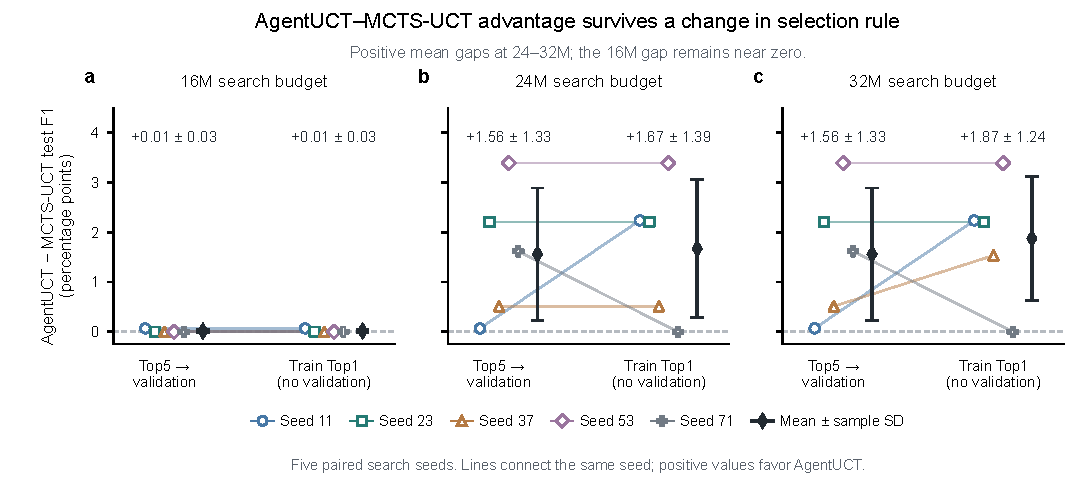
\includegraphics[width=\textwidth]{figures/top1-ablation-20261004/selection-robustness.pdf}
\caption{AgentUCT's advantage over MCTS-UCT persists without validation.
Panels compare paired test-F1 differences under both selection rules at each
budget. Symbols retain all five seeds; summaries show mean $\pm$ sample SD.
Positive values favor AgentUCT. The 16M cutoff mostly reflects initialization;
repeated endpoints across budgets reuse complete measurements.}
\label{fig:selection-robustness}
\Description{Paired AgentUCT minus MCTS-UCT test F1 at three search budgets under validation selection and direct training Top1 selection. The positive mean advantage at 24M and 32M persists under both rules.}
\end{figure*}

\begin{figure*}[t]
\centering
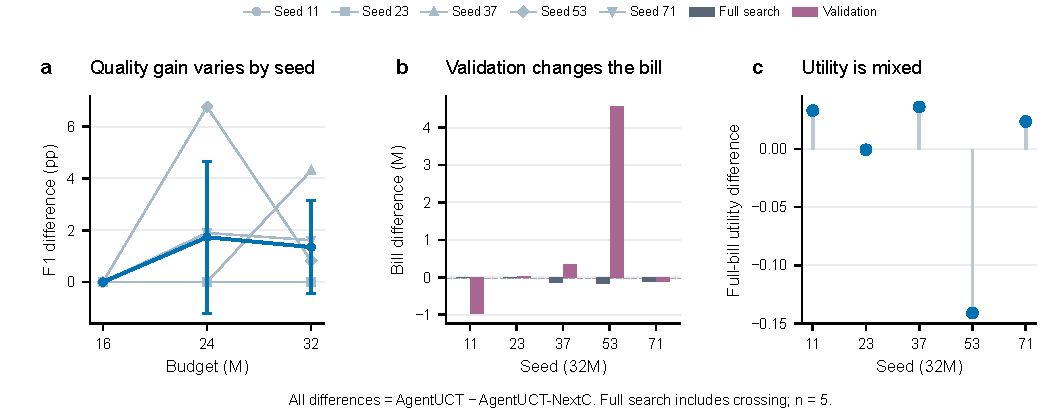
\includegraphics[width=\textwidth]{figures/rag-budget-overlay-20261004/completion-tradeoff.pdf}
\caption{Completion pricing relative to AgentUCT-NextC. (a) Paired test-F1
differences at each budget, with all five seeds and the mean $\pm$ sample SD.
(b) Actual full-search and validation-bill differences at 32M, including the
crossing evaluation in search. (c) Auxiliary full-bill utility differences for
the same five seeds. Positive quality and cost differences respectively mean
higher F1 and a higher bill; positive utility means higher $J$.}
\label{fig:completion-tradeoff}
\Description{Three panels show AgentUCT minus AgentUCT-NextC in test F1, full search and validation cost, and full-bill utility, retaining all five seeds.}
\end{figure*}

\begin{table}[t]
\centering\small\setlength{\tabcolsep}{3pt}
\caption{A saved decision at seed 53, iteration 9. Both actions have
$N=1$ and exploration bonus 2.075225. Cost is predicted remaining work in
M weighted tokens; the final index subtracts $2\widehat b/C_{\rm ref}$.}
\label{tab:completion-choice}
\begin{tabular}{lrrr}
\toprule
Query action & $Q+\mathrm{bonus}$ & Cost (M) & Final index\\
\midrule
Identity & 2.7265 & 1.7760 & 0.3112\\
Synonyms (selected) & 2.6912 & 1.0157 & 1.3100\\
\bottomrule
\end{tabular}
\end{table}

\begin{figure*}[t]
\centering
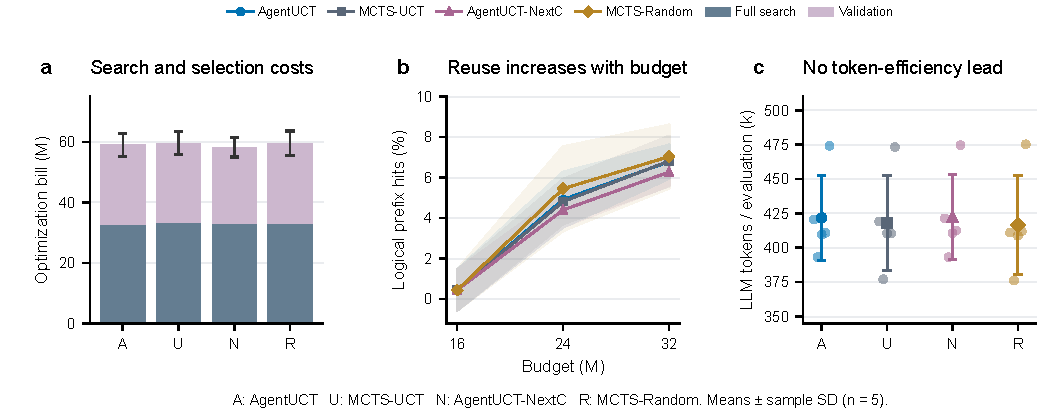
\includegraphics[width=\textwidth]{figures/rag-budget-overlay-20261004/execution-accounting.pdf}
\caption{Execution accounting for all four methods. (a) Mean full optimization
bill at 32M, separated into search and validation; error bars show the sample
SD of the total over five seeds. Test and preparation are separately reported.
(b) Logical hit fractions over all demanded prefix visits at each cutoff,
including zero-cost stages; bands show sample SD. (c) Actual unweighted LLM
input-plus-output tokens per completed evaluation at 32M, with all seeds and
mean $\pm$ sample SD. Logical hits do not measure a no-cache counterfactual.}
\label{fig:execution-accounting}
\Description{Full optimization cost is decomposed into search and validation, followed by logical prefix hit rates and physical LLM tokens per evaluation for the four algorithms.}
\end{figure*}

\begin{figure*}[t]
\centering
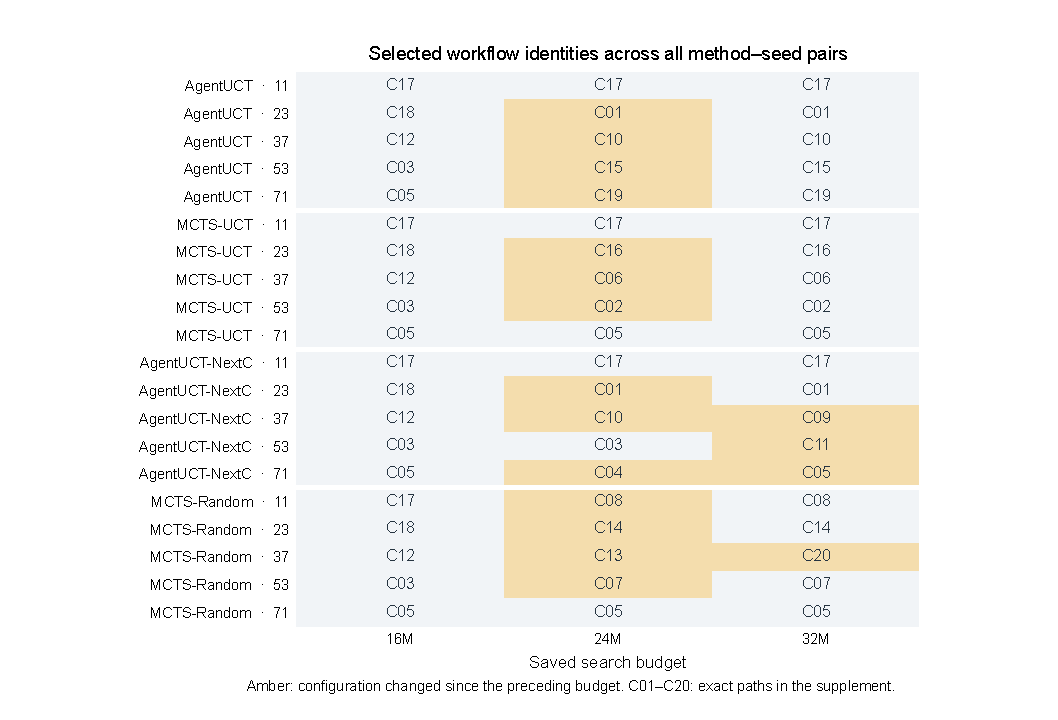
\includegraphics[width=\textwidth]{figures/rag-budget-overlay-20261004/configuration-migration.pdf}
\caption{Budget migration of validation-selected workflows. Rows retain each
method and search seed; columns use the three complete affordable snapshots.
Codes identify exact component sequences in the supplementary configuration
dictionary. Amber marks a changed configuration since the preceding budget.
Equal codes across independent runs identify the same workflow, while its
physical test execution and prediction may differ.}
\label{fig:configuration-migration}
\Description{Twenty method and seed rows show the selected configuration at 16, 24 and 32 million weighted tokens; amber marks changed configurations.}
\end{figure*}

\section{Experimental Protocol and Component Catalogue}
\label{app:experiments}
The completed RAG studies optimize component workflows. AFlow--RAG generates
and charges legal edits within the same grammar. The separate GSM8K study
optimizes generated Python workflows; earlier fixed-library and bounded
generated-workflow pilots remain diagnostic and are excluded from its formal cohort.
Every generative execution role uses the same Qwen3.5-4B checkpoint: query refinement,
progress assessment, listwise reranking, answer generation, workflow review
and repair. The dynamic AFlow study generates and charges Python-workflow edits.
Dedicated embedding models remain retrieval components. All inference runs on
the experiment server. Up to seven GPUs run Qwen workers; the eighth hosts the shared E5, BGE and Qwen
embedding service. Each trial owns its document indices and online caches;
sharing model residency creates no cross-trial reuse credit. Direct small-model component selection is
outside this study.
The deferred planning references specify DeepSeek-V4-Pro and GPT-5.5 as
offline planners, with proposed workflows executed by Qwen3.5-4B. These
references currently have no completed measurements; their protocol separates
planner and execution charges.

The paired RAG evaluator fixes bfloat16 inference, greedy generation in fixed
query groups with model batches capped at four, encoder batches capped at eight for both index construction and
query encoding, model context limits and deterministic ranking tie rules.
Document indices are built under this common configuration before search.
Changing these evaluator settings defines a separate experimental cohort.
The completed batch cohort started all four methods and five seeds afresh; earlier
single-request search trees and generated responses are not imported.

\subsection{Conceptual comparison with related optimizers}
Table~\ref{tab:related} summarizes the design models discussed in Related Work.
The completed five-seed RAG comparisons contain AgentUCT, MCTS-UCT,
AgentUCT-NextC, AgentUCT-StaticFull, MCTS-Random, adapted AFlow,
uniform-terminal search, FLASH*--RAG (TPE), EEIPU--RAG, LaMBO--RAG and
MSBO--RAG. The separate formal GSM8K study
compares AFlow, MCTS-UCT and AgentUCT within the same dynamic execution system;
its earlier pilot supplies execution evidence only.
\begin{table*}[t]
\centering\small
\caption{Conceptual comparison of cost and execution-state models, not an
empirical benchmark. Rows describe the cited methods' allocation mechanisms
and analysis targets; Related Work supplies their references.}
\label{tab:related}
\begin{tabularx}{\textwidth}{@{}l XXX@{}}
\toprule
Method & Cost and reusable state & Allocation statistic & Analysis target\\
\midrule
FLASH & Pipeline-prefix intermediates; LRU eviction & Cost-sensitive BO acquisition & Efficient pipeline optimization\\
EEIPU & Selected memoized prefixes; stage-cost GPs & EI and inverse remaining cost & Budgeted BO with memoization\\
LaMBO & Modular change from the preceding configuration & Slowly moving bandit and local BO & Switching-cost-regularized regret\\
MSBO & Inventory of partial cascades and observations & Stage models; start or advance a sample & Multistage evaluation efficiency\\
AFlow & Generated program and execution feedback & Parent score/uniform mixture & Workflow optimization\\
AgentUCT & Persistent qid--prefix demands shared by panels & Raw ancestor returns and completion-cost price & Demand-information boundary; same-state tradeoff; fixed-table quality regret\\
\bottomrule
\end{tabularx}
\end{table*}

\subsection{Direct AFlow comparison in the common RAG space}
The AFlow adapter proposes edits within the same 61,344-workflow grammar,
using Qwen3.5-4B and completed training feedback. Its parent selection retains
the score/uniform mixture. Proposal and repair calls enter the actual search
bill, and every accepted workflow completes the full 150-question panel
before it can supply feedback for another proposal. All methods use the same
three actual-cost cutoffs and Top5--validation--test selection. This comparison
tests allocation within a common component space; the generated Python-workflow
experiment on GSM8K tests transfer within the AFlow execution system.

AgentUCT exceeds the adapted AFlow policy at 24M and 32M in all five paired
seeds (Table~\ref{tab:completed-aflow-paired}). At 32M, the differences are
1.24, 3.71, 3.25, 3.22 and 0.18 percentage points for seeds
11, 23, 37, 53 and 71, respectively, with mean $2.32\pm1.53$ points.
AFlow's five-seed mean F1 is $65.93\pm1.91\%$, $66.38\pm1.24\%$
and $67.25\pm1.57\%$ at 16M, 24M and 32M.
For seeds 11 and 23, AFlow retains 19 and 21 complete evaluations, respectively,
compared with AgentUCT's 18 and 19: the quality advantage in these runs does
not require more completed evaluations. At 16M, AFlow leads by 2.61 points
in seed 53, where the cutoff primarily covers common initialization for
AgentUCT and MCTS-UCT. At 16M, AgentUCT leads in three seeds and AFlow
in two; the result does not support superiority at every budget.

\begin{table*}[t]
\centering\small
\caption{Completed paired AFlow--RAG comparisons. Entries are primary test
F1 in percent under the common actual search-budget ceiling and Top5
validation protocol. The methods are compared directly by their test F1.
All five matched seeds are shown; repeated budget endpoints are not
independent measurements.}
\label{tab:completed-aflow-paired}
\begin{tabular}{@{}rrrrr@{}}
\toprule
Seed & Budget (M) & AgentUCT & MCTS-UCT & AFlow\\
\midrule
11 & 16 & 69.51 & 69.44 & 66.25\\
11 & 24 & 69.51 & 69.44 & 65.76\\
11 & 32 & 69.51 & 69.44 & 68.27\\
23 & 16 & 67.05 & 67.05 & 65.76\\
23 & 24 & 69.52 & 67.32 & 65.76\\
23 & 32 & 69.52 & 67.32 & 65.81\\
37 & 16 & 69.20 & 69.20 & 63.22\\
37 & 24 & 69.20 & 68.69 & 65.76\\
37 & 32 & 69.20 & 68.69 & 65.95\\
53 & 16 & 63.21 & 63.21 & 65.81\\
53 & 24 & 69.97 & 66.58 & 66.02\\
53 & 32 & 69.97 & 66.58 & 66.75\\
71 & 16 & 68.01 & 68.01 & 68.59\\
71 & 24 & 69.63 & 68.01 & 68.59\\
71 & 32 & 69.63 & 68.01 & 69.45\\
\bottomrule
\end{tabular}

\end{table*}

Complete search bills, including proposal and repair, are 32.187M and
33.429M weighted tokens for seeds 11 and 23. Their last affordable 32M
snapshots cost 30.195M and 31.881M. The complete crossing steps cost 1.991M
and 1.549M, whereas the amounts above the ceiling are 0.187M and 1.429M.
Validation costs a further 29.319M and 20.773M; test costs 9.698M and 5.552M.
All 42 and 39 rejected proposal rounds remain charged. Previously paid
input-index preparation is cited separately, including the reused indices
in seed 23.
For seeds 37 and 53, complete search costs 32.739M and 33.184M; the 32M
snapshots retain 31.013M and 31.542M. Their full crossing evaluations cost
1.726M and 1.642M, with 0.739M and 1.184M above the ceiling.
Validation costs 31.315M and 21.950M, and test costs 8.992M and 8.289M.
All 26 and 42 rejected proposal rounds remain charged; previously paid
input preparation is accounted for separately.
For seed 71, complete search costs 33.769M and the 32M snapshot retains
31.814M. The full crossing evaluation costs 1.955M, of which 1.769M is
above the ceiling. Validation and test cost 30.119M and 7.741M,
respectively. All twelve rejected proposal rounds remain charged.
The five completed runs retain 21.0 evaluations on average at 32M,
compared with AgentUCT's 17.6. These counts concern affordable complete
evaluations; all crossing charges remain in the full bills.

\subsection{Completed common-space extension measurements}
Table~\ref{tab:completed-seed11-extensions} reports each completed optimizer
trial alongside the 32M test F1 of AgentUCT and MCTS-UCT with the same seed.
The shared grammar, evaluator, actual-cost cutoffs and held-out selection
protocol are fixed; each optimizer retains its declared initialization and
allocation policy. The table reports all 25 individual trials for these five controls. The original four-method comparison, AFlow and
AgentUCT-StaticFull have separate completed five-seed comparisons.
Uniform-terminal, FLASH*, EEIPU, LaMBO and MSBO have complete five-seed cohorts
(Table~\ref{tab:uniform-flash-complete}).
MSBO--RAG reaches 69.93\% at 32M in seed 23, 0.41 percentage points above
AgentUCT's 69.52\% with the same seed. Across all five seeds, AgentUCT leads
MSBO by $2.13\pm2.51$ points at 32M, with four wins and one loss.

\begin{table*}[t]
\centering\small
\caption{Completed common-space optimizer trials. F1 is primary test performance
in percent after Top5 validation selection. The AgentUCT and MCTS-UCT columns
show their same-seed 32M test F1 directly. $N_{32}$ and cost count complete evaluations and M weighted-token units
in the last affordable 32M snapshot. Each row is one trial; repeated endpoints
across budgets reuse measurements.}
\label{tab:completed-seed11-extensions}
\begin{tabular}{@{}lrrrrrrrr@{}}
\toprule
Method & Seed & 16M F1 & 24M F1 & 32M F1 & \shortstack{AgentUCT\\32M F1} & \shortstack{MCTS-UCT\\32M F1} & $N_{32}$ & Cost (M)\\
\midrule
FLASH*--RAG (TPE) & 11 & 67.79 & 66.55 & 66.55 & 69.51 & 69.44 & 19 & 31.761\\
FLASH*--RAG (TPE) & 23 & 64.15 & 65.67 & 66.28 & 69.52 & 67.32 & 24 & 31.556\\
FLASH*--RAG (TPE) & 37 & 65.38 & 67.47 & 67.47 & 69.20 & 68.69 & 17 & 31.744\\
FLASH*--RAG (TPE) & 53 & 66.86 & 66.86 & 67.91 & 69.97 & 66.58 & 13 & 30.497\\
FLASH*--RAG (TPE) & 71 & 68.25 & 68.25 & 68.25 & 69.63 & 68.01 & 22 & 31.980\\
\addlinespace
EEIPU--RAG & 11 & 67.95 & 67.95 & 67.26 & 69.51 & 69.44 & 17 & 29.469\\
EEIPU--RAG & 23 & 67.72 & 68.09 & 68.09 & 69.52 & 67.32 & 24 & 30.432\\
EEIPU--RAG & 37 & 69.13 & 68.05 & 66.01 & 69.20 & 68.69 & 19 & 31.914\\
EEIPU--RAG & 53 & 67.53 & 67.53 & 67.53 & 69.97 & 66.58 & 24 & 29.968\\
EEIPU--RAG & 71 & 63.43 & 69.31 & 67.59 & 69.63 & 68.01 & 22 & 31.227\\
\addlinespace
LaMBO--RAG & 11 & 65.18 & 64.60 & 65.63 & 69.51 & 69.44 & 37 & 31.112\\
LaMBO--RAG & 23 & 66.16 & 66.36 & 66.36 & 69.52 & 67.32 & 35 & 30.859\\
LaMBO--RAG & 37 & 64.72 & 69.59 & 67.29 & 69.20 & 68.69 & 19 & 29.481\\
LaMBO--RAG & 53 & 64.10 & 65.07 & 69.19 & 69.97 & 66.58 & 26 & 31.037\\
LaMBO--RAG & 71 & 63.72 & 63.72 & 62.07 & 69.63 & 68.01 & 34 & 31.491\\
\addlinespace
MSBO--RAG & 11 & 67.82 & 68.59 & 68.59 & 69.51 & 69.44 & 14 & 29.855\\
MSBO--RAG & 23 & 67.08 & 69.93 & 69.93 & 69.52 & 67.32 & 17 & 26.855\\
MSBO--RAG & 37 & 66.77 & 68.66 & 66.64 & 69.20 & 68.69 & 12 & 27.007\\
MSBO--RAG & 53 & 67.51 & 69.02 & 68.59 & 69.97 & 66.58 & 15 & 30.116\\
MSBO--RAG & 71 & 66.81 & 63.43 & 63.43 & 69.63 & 68.01 & 19 & 31.010\\
\addlinespace
Uniform-terminal search & 11 & 66.76 & 66.76 & 69.33 & 69.51 & 69.44 & 18 & 30.749\\
Uniform-terminal search & 23 & 66.28 & 66.28 & 66.28 & 69.52 & 67.32 & 16 & 31.269\\
Uniform-terminal search & 37 & 67.99 & 67.99 & 67.99 & 69.20 & 68.69 & 20 & 31.268\\
Uniform-terminal search & 53 & 67.78 & 65.78 & 65.17 & 69.97 & 66.58 & 16 & 31.550\\
Uniform-terminal search & 71 & 66.58 & 66.58 & 67.11 & 69.63 & 68.01 & 14 & 31.804\\
\bottomrule
\end{tabular}

\end{table*}

\begin{table*}[t]
\centering\small
\caption{Complete five-seed comparisons with five common-space sampling, surrogate and stage-allocation controls. Test F1 is directly compared with AgentUCT at each budget, as mean $\pm$ sample SD across five search seeds. Mean $N$ counts affordable complete evaluations for the listed method; budgets can reuse endpoints and are not independent replications.}
\label{tab:uniform-flash-complete}
\begin{tabular}{@{}llrrr@{}}
\toprule
Method & Budget & AgentUCT F1 (\%) & Method F1 (\%) & Mean $N$\\
\midrule
Uniform-terminal & 16M & $67.40\pm2.54$ & $67.08\pm0.76$ & 8.2\\
Uniform-terminal & 24M & $69.57\pm0.28$ & $66.68\pm0.82$ & 12.4\\
Uniform-terminal & 32M & $69.57\pm0.28$ & $67.18\pm1.59$ & 16.8\\
FLASH*--RAG (TPE) & 16M & $67.40\pm2.54$ & $66.49\pm1.70$ & 8.0\\
FLASH*--RAG (TPE) & 24M & $69.57\pm0.28$ & $66.96\pm0.97$ & 13.2\\
FLASH*--RAG (TPE) & 32M & $69.57\pm0.28$ & $67.29\pm0.85$ & 19.0\\
EEIPU--RAG & 16M & $67.40\pm2.54$ & $67.15\pm2.17$ & 12.6\\
EEIPU--RAG & 24M & $69.57\pm0.28$ & $68.19\pm0.67$ & 16.2\\
EEIPU--RAG & 32M & $69.57\pm0.28$ & $67.29\pm0.78$ & 21.2\\
LaMBO--RAG & 16M & $67.40\pm2.54$ & $64.78\pm0.96$ & 11.4\\
LaMBO--RAG & 24M & $69.57\pm0.28$ & $65.87\pm2.29$ & 20.6\\
LaMBO--RAG & 32M & $69.57\pm0.28$ & $66.11\pm2.62$ & 30.2\\
MSBO--RAG & 16M & $67.40\pm2.54$ & $67.20\pm0.46$ & 8.8\\
MSBO--RAG & 24M & $69.57\pm0.28$ & $67.93\pm2.57$ & 12.4\\
MSBO--RAG & 32M & $69.57\pm0.28$ & $67.44\pm2.53$ & 15.4\\
\bottomrule
\end{tabular}

\end{table*}

At 32M, the paired AgentUCT advantages over EEIPU and LaMBO are
$2.27\pm0.64$ and $3.46\pm2.58$ percentage points (mean $\pm$ sample SD),
positive in every seed. LaMBO nevertheless exceeds AgentUCT by 0.389 points
in seed 37 at 24M. The fifteen budget cells for EEIPU and LaMBO reference
twelve and thirteen distinct complete selected test measurements,
respectively; repeated endpoints do not supply independent replications.
In seed 71, full search/validation/test bills are
33.186M/41.059M/15.392M for EEIPU and 33.987M/20.580M/7.764M for LaMBO.
Their complete crossing evaluations cost 1.959M and 2.497M, whereas their
32M overshoots are 1.186M and 1.987M. Paid input preparation is separate;
these bills cover all three cutoffs' measurement campaign and do not define
the original 32M-only optimization utility.

FLASH*--RAG uses two D-optimal initial evaluations, three linear-EIPS
evaluations and fifteen TPE evaluations in seed 11. The pruned tuning
domain contains 2,304 legal workflows. The asterisk denotes the declared
common-space adaptation. Complete search costs 33.716M weighted tokens;
validation and test cost 33.036M and 7.452M, respectively. The last complete
evaluation adds 1.955M, with 1.716M above the 32M ceiling. EEIPU--RAG performs
five warmup and thirteen acquisition evaluations in seed 11, with complete search,
validation and test bills of 33.310M, 41.727M and 15.611M. Its runtime
handoff preserves the completed search and all previously paid calls.
Uniform-terminal search samples legal complete workflows without replacement
and evaluates nineteen of them in seed 11. Its search, validation and test
bills are 32.526M, 41.589M and 9.105M; the last complete evaluation adds
1.778M, taking search 0.526M above the ceiling. It uses training evaluations
and the common Top5 protocol, whereas the separate fifty-workflow reference
directly measures a prespecified test distribution.
Shared input-index preparation is cited separately for these methods.
LaMBO--RAG completes 38 training panels in seed 11: five warmup evaluations
and 33 local GP-UCB evaluations under slowly moving region sampling.
Its 16M, 24M and 32M snapshots retain 14, 25 and 37 complete evaluations,
with test F1 of 65.18\%, 64.60\% and 65.63\%. At 32M the retained bill
is 31.112M; full search costs 33.058M, including a complete 1.946M
crossing evaluation and 1.058M above the ceiling. These bills describe seed 11.
The adaptation uses fixed partition depths $(1,1)$, a finite categorical
domain and persistent WTB reuse. Its switching-cost helper is not called;
the measured execution bill is not the numerical switching-cost objective
of the original algorithm. Saved region probabilities, conditional sampling,
lazy-prefix eligibility and completed-feedback updates are audited;
unrecorded GP acquisition rankings and SMB random symbols are not reconstructed.
MSBO--RAG completes 26 stages in seed 11: twelve evidence stages and
fourteen terminal evaluations. Every stage joins all 150 training questions
before its feedback enters the optimizer. Its primary snapshots retain
9, 10 and 14 complete workflows at 16M, 24M and 32M; test F1 is
67.82\%, 68.59\% and 68.59\%. The corresponding terminal-boundary bills
are 13.527M, 19.058M and 29.855M. An evidence-only snapshot can contain
additional paid work but cannot supply a new terminal quality observation.
Full search costs 33.277M, including the final evidence-only stage of
3.422M; the amount above 32M is 1.277M. Validation and test cost 33.994M
and 12.352M across the three-cutoff measurement campaign. The stage audit
checks native evidence proxies, per-question reuse of the six-action prefix
and complete-panel updates. It does not reconstruct unsaved GP candidate
rankings or Monte Carlo acquisition draws.
In seed 71, MSBO completes 34 stages: fifteen evidence stages and
nineteen terminal evaluations. Its 32M primary and auxiliary snapshots
both end at stage 33 with a bill of 31.010M. The final evidence stage
costs 1.019M, taking full search to 32.029M; the overshoot is 0.029M.
Validation and test cost 28.610M and 6.970M across the three cutoffs.
The 5.613M cost of all unadvanced evidence inventory spans the full search
and is distinct from this final crossing stage. Paid input preparation
remains separate. Across the five seeds, the fifteen MSBO budget cells
reference twelve complete selected test measurements; statistical
replication remains at the five search seeds.

In seed 23, MSBO completes thirteen evidence stages and seventeen terminal
evaluations. Its 32M primary snapshot ends at stage 28 with a bill of
26.855M. Stage 29 adds evidence and raises the bill to 30.284M without
another complete workflow evaluation; it belongs to the auxiliary snapshot.
Stage 30 costs 3.558M and crosses the ceiling, bringing full search to
33.842M. The 6.987M paid after the last terminal snapshot covers both
evidence stages, whereas the amount above the ceiling is 1.842M.
Validation and test cost 32.506M and 9.209M, respectively, across the
three-cutoff measurement campaign. All of these charges are retained.
These are individual-seed measurements.
For FLASH* and EEIPU, saved traces establish the training observations, selected paths, phase
boundaries and downstream selection. They do not retain the complete
acquisition rankings or random-draw transcript, so the audit does not claim
to reconstruct every numerical argmax.

\subsection{The RAG execution contract}
The main grammar performs one retrieval round and chooses a query strategy,
retriever, evidence-selection rule and retrieval width. Query choices include the current query,
pseudo-document-only retrieval, Query2doc with one or three copies of the
current query followed by its pseudo-document, two-query decomposition,
a concise rewrite, two synonymous rewrites, and HyDE. Synonymous rewrites
preserve one information need; decomposition splits it into subquestions.
Multi-round retrieval is deferred to a separate lower-priority ablation.

Ordinary queries have 30 retriever options: BM25, E5, Qwen embedding,
the original four-way RRF, five BGE-M3 dense/sparse mixtures with dense weights
$0,0.25,0.5,0.75,1$, 15 RRF source-set/constant combinations,
and six weighted fusions.
The five RRF source sets are BM25+E5, BM25+BGE, BM25+Qwen,
E5+BGE, and BM25+E5+BGE+Qwen; each uses $k\in\{10,60,100\}$.
BGE denotes its dense representation in these five sets.
Weighted fusion combines BM25 with E5 or Qwen. Each source's scores are
min--max normalized over the candidate documents; constant scores map to zero.
The BM25 weight is $\alpha\in\{0.25,0.5,0.75\}$ and the dense weight is $1-\alpha$.
HyDE instead selects one of three passage encoders: E5, BGE dense or Qwen.
Generated passages guide retrieval and never enter the evidence pool as sources.

Evidence selection uses relevance or MMR with relevance weight
$0.3,0.6,0.9$; retrieval width is $2,4,6,10$, capped by the candidate count.
The workflow then chooses identity or Qwen reranking and selects the first
$2,4,6$ available documents, capped by the evidence count. It preserves their
full source text and applies one CPU-only ordering: ranked, reversed, or ends.
The ends order alternates relevance ranks between the front and back, giving
$1,3,5,6,4,2$ for six documents. All three orders preserve the selected set.
For two documents, ends and ranked coincide. Ordering performs no model call;
the selected ordered context is passed to one final answer-generation stage.
There is no separate model-based order evaluator. Format retries follow the
same charged retry contract as every other method.

The retrieval block has $A_0=(7\cdot30+3)\cdot4\cdot4=3408$ choices.
Two rerankers, three evidence widths and three orders give
$18A_0=61{,}344$ syntactic terminal workflows. The final answer action is
uniquely determined by the selected width and adds no choice factor.
Input-specific coincidences and width truncation can make different paths
execute the same behavior. This count does not assert distinct effective policies.
The finite-tree theorem concerns the declared terminal grammar.

The first retrieval retains the grounded evidence assessment used in the
loop-value diagnostic: Qwen selects document and sentence identifiers, and the
adapter recovers exact source text. Its costs and retries are recorded.
Identity reranking prioritizes cited documents within the retrieved evidence;
the alternative reranker uses the same Qwen model. Neither controller receives
gold answers or supporting-document labels. WTB checkpoints preserve the selected
documents, their full text, the chosen order and the answer state. Candidates
with different orders share the prefix through evidence selection and execute
their own answer suffix. Compression is excluded from the main grammar.

\subsection{Paper-grounded reference workflows}
\label{app:paper-workflow-references}
The earlier Agent-UCT study compared searched configurations with fixed
framework presets, then examined held-out quality, chosen components and
execution costs~\citep{li2026agentuct}. We retain these questions with three
published pipelines. Each cited paper already combines at least two of the
mechanisms represented in our grammar: Query2doc combines generated query
expansion with lexical retrieval; HyDE combines hypothetical-document
generation with dense retrieval; RankGPT combines candidate retrieval with
listwise language-model reranking.

All references use the same candidate documents, grounded evidence
assessment, one retrieval round, retrieval width six, four retained documents,
ranked context and Qwen3.5-4B answer generation. Unspecified slots use the
original query, BM25, relevance selection and identity reranking. The common
identity reranker prioritizes documents cited by the grounded assessment,
as in the search grammar. These are shared-space adaptations of the three
published retrieval pipelines, evaluated as complete QA workflows.

\begin{table}[t]
\centering\small
\caption{Three fixed references, each based on a published combination of
implemented mechanisms. All are evaluated on the same 300 primary test
questions without training or validation selection. Test F1 is in percent;
each recipe is a single fixed-workflow measurement.}
\label{tab:paper-workflow-recipes}
\begin{tabularx}{\linewidth}{@{}lp{0.26\linewidth}Xr@{}}
\toprule
ID & Published pipeline & Fixed component choices & Test F1\\
\midrule
P01 & Query2doc--BM25~\citep{wang2023query2doc} & \path{query.query2doc:q=3} then \path{retriever.bm25}. & 61.60\\
P02 & HyDE--E5~\citep{gao2023hyde} & \path{query.hyde} then \path{retriever.hyde_e5}. & 62.89\\
P03 & RankGPT-style BM25--Qwen~\citep{sun2023rankgpt} & \path{retriever.bm25} then \path{reranker.qwen3}. & 62.53\\
\bottomrule
\end{tabularx}
\end{table}

The three adapted references reach 61.60--62.89\% test F1, below the
69.57\% mean for AgentUCT's selected workflows at 32M. The selected workflows
improve on these specified recipes; the matched MCTS-UCT comparison isolates the
allocation change.
Their complete test-execution bills are 3.338M, 2.971M and 5.113M weighted
tokens, respectively, including one excluded sentinel per recipe.
Previously paid input-index preparation is referenced separately. These
measurements supply no across-run SD. The completed four-contrast analysis
includes these three fixed recipes and the mean of all fifty random workflows.

Query2doc uses our Qwen JSON prompt and three query copies, compared with
the original four-shot prompt, text-davinci-003 and five copies.
HyDE uses one Qwen-generated passage with E5 document-side encoding,
compared with the original InstructGPT and Contriever/mContriever setup.
It does not average multiple generated-document embeddings; E5's training
also means this adapter does not inherit an unsupervised-retrieval claim.
P03 uses a single listwise window of at most six documents with Qwen3.5-4B,
compared with RankGPT's BM25 top-100 candidates and GPT sliding-window
protocol. Up to two format attempts are allowed, all executed attempts are
charged, and two invalid orders retain the common fusion order with a
recorded fallback. No retriever or reranker is retrained for this comparison.

The exact nine-action paths are frozen in
\path{configs/rag-followup-v2/fixed-test-manifest.json}. An independent
native-grammar check confirms all three are legal terminal workflows.
The former twelve-recipe catalogue and additional component sensitivity
sweep are outside this accelerated experiment plan.

Fifty further complete workflows were sampled uniformly without replacement
from all 61,344 legal terminals, using seed 20261004 before their test
execution. Every sampled workflow was evaluated. Mean test F1 was
$60.58\pm5.22\%$ across workflows, the median was $62.11\%$, and the
interquartile range was $57.19$--$65.20\%$. The full observed range was
$48.43$--$68.39\%$; no draw was selected by test quality. Mean EM was
$46.39\pm4.88\%$. This no-search random-composition reference is distinct
from MCTS-Random allocation and from uniform-terminal search, which pays
for training evaluations and uses Top5--validation selection.
The three paper references and fifty random workflows require 15,900
primary question--workflow executions before reuse, plus separate sentinels.
All 15,900 primary outcomes and 53 sentinel outcomes completed. The fifty
random workflows incurred 164.392M weighted-token units of test execution;
the three fixed recipes incurred 11.422M. The combined 175.815M bill
contains 143,630 settled physical calls, with no failed calls or new input
preparation. This is the cost of measuring the reference distribution,
separate from an optimizer's search and validation bill.

\begin{figure}[t]
\centering
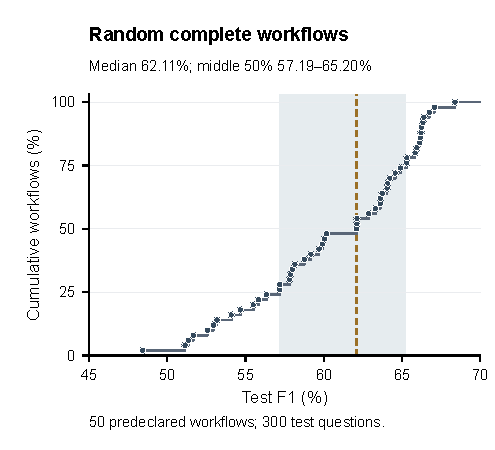
\includegraphics[width=3.3in]{figures/rag-extended-analysis-20261004/quality/random-composition-distribution.pdf}
\caption{Test F1 of all fifty prespecified random complete workflows. Each
point is one workflow on the same 300 primary questions. The gray band marks
the interquartile range and the dashed line the median; neither is a
confidence interval. The distribution describes unoptimized composition;
no draw is promoted to a selected baseline.}
\label{fig:random-composition-distribution}
\Description{All fifty sampled complete workflows are shown on a common test F1 axis, retaining the full observed distribution.}
\end{figure}

Strong-model planning was specified for native \path{deepseek-v4-pro} and
OpenRouter \path{openai/gpt-5.5}, with five plans each and high reasoning
effort~\citep{deepseek2026v4pro,openai2026gpt55}. Both receive identical task
instructions, grammar, component descriptions and three frozen training
examples, with no test inputs or quality feedback. The first generation
requests returned insufficient balance and regional unavailability,
respectively. These references are deferred; provider rejection is not a
zero-quality workflow measurement.

The active paired-test family contains four contrasts: the three fixed
recipes and the mean across all fifty random workflows, each against
AgentUCT's mean per-question F1 vector across its five seeds at 32M.
Holm adjustment covers this family.
The question is the paired unit; search-seed and random-workflow variation
are displayed separately. Full design details appear in
Section~\ref{sec:workflow-references}.

\begin{table}[t]
\centering\small\setlength{\tabcolsep}{3pt}
\caption{Question-paired reference comparisons at the fixed 32M endpoint.
$\Delta$ is AgentUCT's five-seed mean minus the reference. Intervals are
pointwise 95\% question-bootstrap intervals conditional on the observed
workflows; Holm adjusts only the four two-sided sign-randomization $p$ values.}
\label{tab:reference-paired-effects}
\begin{tabular}{@{}lrrrr@{}}
\toprule
Reference & F1 (\%) & $\Delta$ (pp) & 95\% CI (pp) & Holm $p$\\
\midrule
P01: Query2doc & 61.60 & +7.97 & [4.86, 11.25] & $6.0\!\times\!10^{-5}$\\
P02: HyDE & 62.89 & +6.68 & [3.59, 9.94] & $6.0\!\times\!10^{-5}$\\
P03: RankGPT-style & 62.53 & +7.04 & [3.72, 10.52] & $6.0\!\times\!10^{-5}$\\
Random mean (50) & 60.58 & +8.98 & [7.17, 10.93] & $4.0\!\times\!10^{-5}$\\
\bottomrule
\end{tabular}

\end{table}

The mean differences are 7.97, 6.68 and 7.04 percentage points for the
three fixed pipelines, and 8.98 points for random composition
(Table~\ref{tab:reference-paired-effects}). The random-composition contrast
has a conditional interval of [7.17, 10.93] points. Resampling random
workflows alone gives [7.52, 10.45] points; resampling both random
workflows and questions gives a sensitivity interval of [6.72, 11.53] points,
with the five AgentUCT seeds still fixed. The AgentUCT seed means range
from 69.20\% to 69.97\%, with sample SD 0.28 points; this search-seed
variation is separate from question uncertainty and the 5.22-point spread
across random workflows.

The paired bootstrap used 10,000 draws with seed 20261002. The two-sided
sign randomization used 100,000 draws with seed 20261005 and the
plus-one correction; the random-mean contrast had no sampled value as
extreme as the observed statistic, giving unadjusted $p=1/100001$, not zero.
Workflow-only and crossed workflow--question sensitivities used 10,000
draws each, with seeds 20261006 and 20261007. All resampling moved complete
question vectors together. These numerical choices were recorded before
resampling, after aggregate outcomes had been inspected. The comparisons
are retrospective on the existing panel and require the stated
question-level sign-exchangeability null; they do not establish performance
on new datasets or new search seeds.

\subsection{Allocation and controls}
Search and validation contain 150 and 300 disjoint hard questions from the
official HotpotQA training split. The primary test contains 300 hard questions
from the official validation split. Training and validation use sampling seed
20261003, excluding earlier search, validation, development and calibration
questions; the primary test remains unchanged. Earlier mixed-difficulty
searches are historical diagnostics outside this cohort.
Each method and seed owns one tree over all 150 training questions. A complete
workflow evaluation returns mean answer F1 over these 150 questions and backs
up that single return to the expanded node and its ancestors. The tree retains
its statistics, random state and qid--prefix cache between evaluations.
At each retained actual-cost snapshot, completed distinct workflows are ranked
by training mean F1, with first evaluation breaking ties. The top five are
evaluated on 300 validation questions. Highest validation mean F1 selects the
endpoint, with training rank breaking ties; 300 held-out questions provide the
primary test score. Validation and test scores never enter reward backup.
An unchanged workflow on an unchanged held-out panel is measured once and
referenced by any repeated measurement request.

The core comparison contains MCTS-Random, MCTS-UCT, AgentUCT with
Policy-complete costs, and AgentUCT-NextC. MCTS-UCT supplies the
standard UCB-guided Monte Carlo tree search baseline. MCTS-Random retains the same
tree and raw-return backup but selects children uniformly, independently of
their reward statistics; this is not uniform sampling over terminal workflows. Expansion and
rollout remain uniform. Five paired seeds (11, 23, 37, 53 and 71) define twenty
completed trials. The first eight trials were audited before continuing the
remaining seeds with unchanged settings; all twenty now have saved-trajectory,
accounting and endpoint-selection checks.
New seeds retain the same primary questions and assess search-seed variation.
If their primary scores are used to change the scientific settings, subsequent
results on that panel are exploratory. Independent confirmation of such a
change requires unused hard test questions fixed before execution.
Each method has its own cache and tree, with the same initial state,
controller, model, resource accounting and validation protocol. The
demand-profile theorem also covers selective panels; this fixed full-panel
experiment instantiates its compression case.

AgentUCT-NextC estimates the first positive unpaid execution per query.
Policy-complete prices the complete reward using 16 legal completions sampled
from smoothed historical prefix transitions. They use the same samples at a
common state, isolating the omitted suffix, and share the physical-price
learning rule and current cache observations. Additional allocation-stage
variants, Uniform-complete and the no-cache GPU arm are deferred. A comparison
of incidence and residual prefix totals can use saved states without another
model run; it is not an online search requirement.

Price priors come from independent fixed-path calibration on questions excluded
from search and evaluation. Each completed training evaluation updates physical
cost means and prefix-transition counts. Cache hits produce no cold-price sample.
The model uses qid--prefix, prefix and component means in that order, with a
calibration pseudo-observation. The historical completion law approximates
subsequent demand; it is not the exact current UCT policy expectation.
Evidence selection and CPU ordering have zero model-token price. Width-conditioned
answer prices belong to the final answer edge.

The global scale is 150 times the median calibrated one-query completion bill;
tiny retains this same value. Token receipts are weighted by model parameter
count in billion-parameter-token units. Batch charges use logical request tokens,
including retries and excluding padding; padded slots and physical batch sizes
are recorded separately. The budget is a resource proxy, with no equivalence
to a fixed GPU-time or FLOP budget. Raw tokens, elapsed model time and
estimator CPU time are retained. Index preparation, search, validation and
held-out measurement have separate receipts. Offline checks compare recorded
cost forecasts with the selected continuation's realized bill. Their difference
combines continuation variability and price error; it does not isolate either
source or measure an unselected continuation. No calibrated error radius is claimed.

The frozen protocol specifies five seeds and one 32M weighted-token budget,
the same model context/output limits and an evaluation-count safety cap. Each tiny
configuration changes only its dataset path: it loads three training queries,
one validation query and one development sentinel. Formal measurement excludes
that sentinel from the 300-query primary held-out score. Test F1 and EM,
physical costs and distinct syntactic workflows accompany
the common-budget comparison. Means and sample SDs describe variation across
the five search seeds on the fixed test panel; query--seed pairs are not
treated as independent repetitions.

Validation-selected primary-test F1 at a fixed search budget is the primary
outcome. The search backs up training F1, uses cost-aware UCT for allocation,
and selects the final workflow by validation F1 alone. As an auxiliary diagnostic,
we report endpoint utility $J=F-\lambda_J C_{\mathrm{opt}}/\cref$ using
primary held-out F1, the existing reporting weight $\lambda_J=0.05$, and the
fixed calibration scale $\cref=1{,}470{,}690.0198555747$. The full physical
$C_{\mathrm{opt}}$ includes search, its complete crossing evaluation, and
validation, including failed attempts and retries. Test measurement and common
index preparation have separate bills and are excluded from this declared
optimization utility. A secondary snapshot utility substitutes the retained
search bill and is labeled separately; it does not remove crossing work from
the full-bill utility or physical ledger. Negative $J$ values are possible under
this fixed scale. Neither the reporting weight nor the scale is selected from
test outcomes. Adding a constant would change only the displayed origin;
changing the weight could change rankings. We retain the raw definition and
display same-seed $\Delta J$ against MCTS-UCT in the main five-seed table.
Search and endpoint selection do not optimize this reporting utility. Joint improvements
in $J$ and F1 are empirical questions, distinct from the allocation theorem.
Utility comparisons use one full optimization bill per seed; a shared bill does not create
independent query-level cost observations. We decompose each difference into
the F1 difference and phase-specific cost contributions, further separating
retained search from complete evaluations after the snapshot cutoff. The latter
is the whole evaluation bill, not only the amount above the reporting budget.
A validation-cost
saving is part of end-to-end utility, not evidence that a search-time cost
forecast was accurate. All three baseline comparisons are retained, including
unfavorable differences. An unknown physical charge prevents reporting a
complete utility value.
This comparison concerns allocation among budgeted search methods. It does not
establish that a one-off search investment is preferable to a fixed workflow
with zero optimization cost.

Table~\ref{tab:all-seeds} preserves every primary score and full-bill utility.
All 214 saved adaptive selections occur at the root. This experiment does not
demonstrate deeper recursive selection gains. Native-checkpoint and reuse
checks cover the explicitly sampled trajectories; they do not constitute a
full native-state audit of every invocation.

\begin{table*}[t]
\centering\small
\caption{All twenty 32M runs. Each entry is primary test F1 (\%) / full-bill $J$.}
\label{tab:all-seeds}
\begin{tabular}{rllll}
\toprule
Seed & AgentUCT & MCTS-UCT & AgentUCT-NextC & MCTS-Random\\
\midrule
11 & 69.5109 / $-1.251646$ & 69.4443 / $-1.242602$ & 69.5109 / $-1.284709$ & 69.3527 / $-1.189892$\\
23 & 69.5228 / $-1.262981$ & 67.3162 / $-1.429808$ & 69.5228 / $-1.262340$ & 67.6926 / $-1.432710$\\
37 & 69.1975 / $-1.164197$ & 68.6871 / $-1.157955$ & 64.8892 / $-1.200446$ & 69.4880 / $-1.165447$\\
53 & 69.9657 / $-1.415753$ & 66.5768 / $-1.434304$ & 69.1490 / $-1.274501$ & 69.4550 / $-1.412869$\\
71 & 69.6305 / $-1.456986$ & 68.0144 / $-1.470387$ & 68.0144 / $-1.480661$ & 68.0144 / $-1.474790$\\
\bottomrule
\end{tabular}
\end{table*}

The five-seed AgentUCT-minus-baseline mean $\Delta J$ is
$+0.03670$ against MCTS-UCT, $-0.00978$ against AgentUCT-NextC and
$+0.02483$ against MCTS-Random. Table~\ref{tab:all-seeds} gives the five underlying
utility pairs for each comparison.
For the random comparison, mean contributions are $+0.00765$ from F1,
$-0.00302$ from retained search, $+0.01273$ from complete crossing evaluations,
and $+0.00747$ from validation. Against MCTS-UCT, the F1, retained-search,
complete-crossing and validation contributions are $+0.01558$, $+0.00084$,
$+0.01450$ and $+0.00578$, respectively. Against AgentUCT-NextC, F1 contributes
$+0.01348$, full search $+0.00294$ and validation $-0.02620$.

Search runs without cost-based admission checks. Every evaluation finishes and
its complete physical bill is recorded. For each reporting budget $B$, retain
the last complete snapshot with cumulative search cost at most $B$. Its tree
statistics, cache membership and shortlist use only that trace prefix.
The evaluation crossing the largest reporting budget also finishes; its work
and overshoot remain in the raw trajectory, and its reward cannot enter an
earlier snapshot. Validation and test measurement use each retained shortlist
and have separately reported costs. Index preparation is also reported
separately. The reporting budgets do not change the selection rule or interrupt
a model call. The finite-tree theorem applies at the retained evaluation
count $n(B)$; it does not assert $O(\log B)$ physical-budget regret.

\subsection{Multi-seed summaries and reporting units}
All budget summaries use the same five search seeds, with one validation-selected
primary outcome per method, seed and budget. Tables report arithmetic means and
sample standard deviations, $s=\sqrt{\sum_{i=1}^{5}(x_i-\bar x)^2/4}$.
The uncertainty bars in the budget and resource figures show this between-seed
spread; they are not standard errors or confidence intervals. A reused endpoint
keeps its original complete test measurement. Reuse across budgets does not
increase the sample size.

For each budget and baseline, we subtract its primary score from AgentUCT's
score for the same seed. Tables report the mean and sample SD of these five
differences, together with wins, ties and losses: the numbers of positive,
zero and negative saved differences. F1 is primary and EM auxiliary.
These summaries describe the observed seed variation on the fixed question
panel. Detailed reporting was added to the frozen runs without changing
allocation or endpoint-selection parameters.

\subsection{Budget-dependent held-out quality}
\label{sec:budget-detail}
All three cutoffs use the same five search seeds and the complete
Top5--validation--primary-test procedure. Table~\ref{tab:budget-quality-full}
reports all method--budget means and sample SDs; the individual seed tables
below preserve the complete sixty outcomes. Early snapshots were read from
frozen completed search prefixes. Only missing validation panels and newly
selected primary endpoints were executed, in separate measurement caches.
No later rewards, prices or execution-cache entries were imported into search.
Across both early-budget campaigns, 242,293 new physical calls incurred
375.606M weighted-token units. These are additional measurement costs, not
observed historical early-stopping optimization bills. We therefore do not
construct 16M or 24M values of $J$.

\begin{table}[htbp]
\centering\small
\caption{Complete matched-five-seed budget analysis. Primary test F1 and EM
are reported as mean $\pm$ sample SD. Each method--budget row has five seeds;
reused test measurements across budgets are not additional independent trials.}
\label{tab:budget-quality-full}
% Sample SD over five seeds (ddof=1); fixed test panel.
\begin{tabular}{rlcc}
\toprule
Budget (M) & Method & F1 (\%) & EM (\%) \\
\midrule
16 & AgentUCT & $67.40 \pm 2.54$ & $52.33 \pm 2.22$ \\
16 & MCTS-UCT & $67.38 \pm 2.52$ & $52.27 \pm 2.14$ \\
16 & AgentUCT-NextC & $67.40 \pm 2.54$ & $52.33 \pm 2.22$ \\
16 & MCTS-Random & $67.40 \pm 2.54$ & $52.33 \pm 2.22$ \\
24 & AgentUCT & $69.57 \pm 0.28$ & $54.60 \pm 0.15$ \\
24 & MCTS-UCT & $68.01 \pm 1.12$ & $52.47 \pm 1.68$ \\
24 & AgentUCT-NextC & $67.83 \pm 2.69$ & $53.33 \pm 2.44$ \\
24 & MCTS-Random & $68.44 \pm 0.89$ & $53.33 \pm 1.49$ \\
32 & AgentUCT & $69.57 \pm 0.28$ & $54.60 \pm 0.15$ \\
32 & MCTS-UCT & $68.01 \pm 1.12$ & $52.47 \pm 1.68$ \\
32 & AgentUCT-NextC & $68.22 \pm 1.96$ & $53.07 \pm 1.64$ \\
32 & MCTS-Random & $68.80 \pm 0.87$ & $53.73 \pm 1.64$ \\
\bottomrule
\end{tabular}

\end{table}

\begin{figure*}[t]
\centering
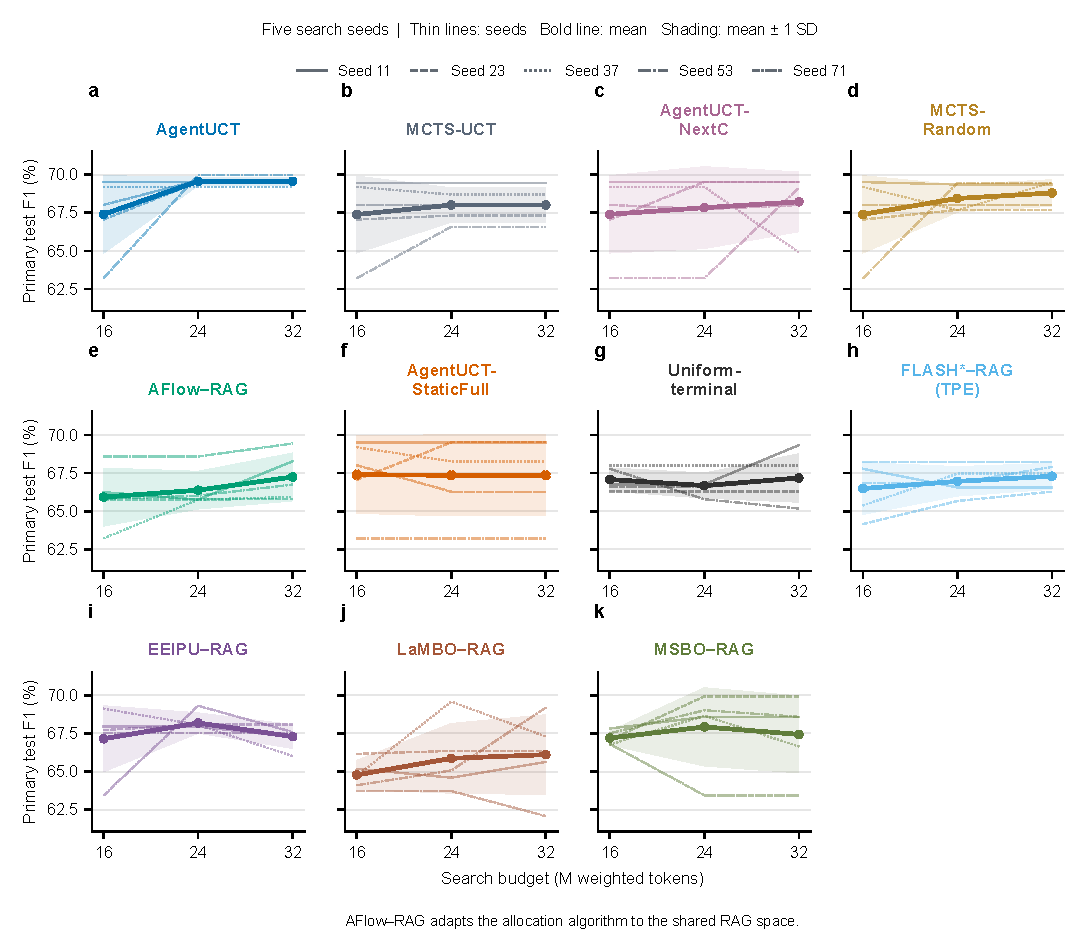
\includegraphics[width=\textwidth]{figures/rag-extended-analysis-20261004/budget/five-seed-budget-test.pdf}
\caption{Individual seed trajectories behind the main budget comparison.
Each method panel shows the same five seeds as thin lines and their mean as
a bold line; shading is $\pm$ one sample SD. Unchanged endpoints within a
trial share a complete test measurement across budgets.}
\label{fig:budget-quality-seeds}
\end{figure*}

The eight initial root evaluations cost 12.287--16.626M weighted tokens across
runs. At 16M, only seed 23 retained two completed adaptive evaluations;
the other four seeds retained none, and seed 53 retained only seven
initialization evaluations.
Consequently, the four methods selected the same within-seed endpoint at 16M.
AgentUCT, AgentUCT-NextC and MCTS-Random had identical test F1; MCTS-UCT's mean differed
by 0.0133 points because seed 11 used a fresh execution of the same workflow.
At 24M, mean F1 was 69.5655\%, 68.0077\%, 67.8342\% and 68.4382\% for
AgentUCT, MCTS-UCT, AgentUCT-NextC and MCTS-Random, respectively. Their 32M values were
69.5655\%, 68.0077\%, 68.2173\% and 68.8006\%.

Table~\ref{tab:initialization-paired-evidence} locates the start of adaptive
allocation within the actual budget. For seeds 23, 37 and 53, the cost term
changes the saved AgentUCT action at its first adaptive decision; for seeds
11 and 71, the first change occurs at evaluation 11. These are comparisons
with the cost-free index in the same saved state, not reconstructed MCTS-UCT
trajectories. Four seeds select different endpoints from MCTS-UCT, with test-F1
gains of 0.51--3.39 points. Seed 11 selects the same endpoint, and its small
difference comes from separate executions. The table connects initialization,
allocation and endpoint changes without attributing an endpoint's F1 gain
to a particular changed action.

\begin{table*}[t]
\centering\small
\caption{Where adaptive allocation becomes observable. A and U denote
AgentUCT and MCTS-UCT. Costs are M weighted tokens. ``First A feedback'' is the
cumulative bill after AgentUCT's first complete adaptive evaluation;
``First changed choice'' is the bill before its first decision whose priced
argmax differs from the same-state cost-free argmax. $\Delta$F1 is AgentUCT
minus MCTS-UCT in percentage points at both 24M and 32M; these budgets reuse the
same endpoint measurement. Configuration IDs resolve in the workflow dictionary.}
\label{tab:initialization-paired-evidence}
\begin{tabular}{@{}rrrrrrll@{}}
\toprule
Seed & Init. A & Init. U & First A feedback & First changed choice & $\Delta$F1 & A config. & U config.\\
\midrule
11 & 13.454 & 13.446 & 16.015 & 17.455 & +0.07 & C17 & C17\\
23 & 12.287 & 12.287 & 13.407 & 12.287 & +2.21 & C01 & C16\\
37 & 13.969 & 13.969 & 16.313 & 13.969 & +0.51 & C10 & C06\\
53 & 16.626 & 16.626 & 17.362 & 16.626 & +3.39 & C15 & C02\\
71 & 13.043 & 13.043 & 16.731 & 20.445 & +1.62 & C19 & C05\\
\bottomrule
\end{tabular}

\end{table*}

The lack of monotonicity has a concrete selection explanation. For
AgentUCT-NextC seed 53, a HyDE workflow ranked fourth in the 24M training
shortlist but sixth at 32M, outside the fixed Top5. Its validation F1 of
73.0699\% exceeded the other eligible winner's 72.4927\%; its primary F1 was
63.2059\%, versus 69.1490\% for the 32M winner. Saved shortlist membership,
validation order, original predictions and official scores were checked.
AgentUCT-NextC seed 37 instead decreased from 69.1975\% at 24M to 64.8892\%
at 32M. A larger budget can change the shortlist and validation winner without
improving that winner's test performance. Neither these outcomes nor the flat
AgentUCT curve was used to tune $\beta$, choose a new stopping budget or
extend the search.

\subsection{AgentUCT versus AgentUCT-NextC}
\label{sec:nextc-detail}
This comparison retains the same completion sampler and price-learning rule
while changing which unpaid costs enter selection. All five paired 16M
endpoints coincide; three coincide at 24M and two at 32M.
The paired F1 difference is $1.73\pm2.93$ points at 24M and
$1.35\pm1.79$ points at 32M. These are means and sample SDs of paired
\emph{differences}, not SDs pooled across independent methods.
Table~\ref{tab:nextc-descriptive} reports this contrast together with EM
and the direction of each seed's difference.

At 32M, AgentUCT used 7.385M raw LLM tokens in its retained search versus
7.399M for AgentUCT-NextC, a 0.18\% difference. Their mean logical hit rates
were 6.79\% and 6.27\%, respectively, with the denominator defined below.
AgentUCT's full search bill was 0.086M weighted tokens lower, but validation
was 0.771M higher. Thus its full optimization bill was 0.684M higher, yielding
the negative mean $\Delta J$ despite higher primary F1. This separates the
observed endpoint-quality result from total optimization expense and does not
establish calibrated forecasts or a general cache-saving mechanism.

\begin{table}[htbp]
\centering\small
\caption{AgentUCT minus AgentUCT-NextC. Differences and their sample SDs
are in percentage points across five paired seeds. W/T/L counts positive,
zero and negative differences; the same rows appear in
Table~\ref{tab:budget-descriptive}.}
\label{tab:nextc-descriptive}
% Descriptive paired seeds only; historical p-value files are preserved.
\begin{tabular}{rlrrrr}
\toprule
$B$ (M) & Contrast / metric & $\Delta$ (pp) & SD (pp) & W/T/L & $n$\\
\midrule
16 & NextC / F1 & +0.00 & 0.00 & 0/5/0 & 5\\
16 & NextC / EM & +0.00 & 0.00 & 0/5/0 & 5\\
24 & NextC / F1 & +1.73 & 2.93 & 2/3/0 & 5\\
24 & NextC / EM & +1.27 & 2.48 & 2/3/0 & 5\\
32 & NextC / F1 & +1.35 & 1.79 & 3/2/0 & 5\\
32 & NextC / EM & +1.53 & 1.71 & 3/2/0 & 5\\
\bottomrule
\end{tabular}

\end{table}
\begin{table}[htbp]
\centering\small\setlength{\tabcolsep}{3pt}
\caption{All paired budget comparisons, AgentUCT minus each baseline.
Differences and sample SDs are in percentage points over five seeds.
W/T/L gives the numbers of seed-level wins, ties and losses. F1 is primary
and EM auxiliary.}
\label{tab:budget-descriptive}
% Descriptive paired seeds only; historical p-value files are preserved.
\begin{tabular}{rlrrrr}
\toprule
$B$ (M) & Contrast / metric & $\Delta$ (pp) & SD (pp) & W/T/L & $n$\\
\midrule
16 & MCTS-UCT / F1 & +0.01 & 0.03 & 1/4/0 & 5\\
16 & NextC / F1 & +0.00 & 0.00 & 0/5/0 & 5\\
16 & MCTS-Random / F1 & +0.00 & 0.00 & 0/5/0 & 5\\
16 & MCTS-UCT / EM & +0.07 & 0.15 & 1/4/0 & 5\\
16 & NextC / EM & +0.00 & 0.00 & 0/5/0 & 5\\
16 & MCTS-Random / EM & +0.00 & 0.00 & 0/5/0 & 5\\
24 & MCTS-UCT / F1 & +1.56 & 1.33 & 5/0/0 & 5\\
24 & NextC / F1 & +1.73 & 2.93 & 2/3/0 & 5\\
24 & MCTS-Random / F1 & +1.13 & 0.74 & 5/0/0 & 5\\
24 & MCTS-UCT / EM & +2.13 & 1.66 & 5/0/0 & 5\\
24 & NextC / EM & +1.27 & 2.48 & 2/3/0 & 5\\
24 & MCTS-Random / EM & +1.27 & 1.44 & 4/0/1 & 5\\
32 & MCTS-UCT / F1 & +1.56 & 1.33 & 5/0/0 & 5\\
32 & NextC / F1 & +1.35 & 1.79 & 3/2/0 & 5\\
32 & MCTS-Random / F1 & +0.76 & 0.92 & 4/0/1 & 5\\
32 & MCTS-UCT / EM & +2.13 & 1.66 & 5/0/0 & 5\\
32 & NextC / EM & +1.53 & 1.71 & 3/2/0 & 5\\
32 & MCTS-Random / EM & +0.87 & 1.57 & 3/0/2 & 5\\
\bottomrule
\end{tabular}

\end{table}

% The generated file contains one complete table per budget.
% Three independent floats in full scope: input directly, without an outer table.
% Actual seed-level scores; each full-scope budget block has 20 rows.
% Same endpoints can reuse a saved test measurement across cutoffs; these are not independent repetitions.
\begin{table}[t]
\centering\small
\setlength{\tabcolsep}{4pt}
\caption{All twenty validation-selected primary outcomes at the 16M search cutoff. F1 and EM are percentages.}
\label{tab:seed-values-b16000000}
\begin{tabular}{rlrrr}
\toprule
Budget (M) & Method & Seed & F1 (\%) & EM (\%) \\
\midrule
16 & AgentUCT & 11 & 69.5109 & 54.6667 \\
16 & AgentUCT & 23 & 67.0514 & 52.3333 \\
16 & AgentUCT & 37 & 69.1952 & 54.0000 \\
16 & AgentUCT & 53 & 63.2059 & 49.0000 \\
16 & AgentUCT & 71 & 68.0144 & 51.6667 \\
16 & MCTS-UCT & 11 & 69.4443 & 54.3333 \\
16 & MCTS-UCT & 23 & 67.0514 & 52.3333 \\
16 & MCTS-UCT & 37 & 69.1952 & 54.0000 \\
16 & MCTS-UCT & 53 & 63.2059 & 49.0000 \\
16 & MCTS-UCT & 71 & 68.0144 & 51.6667 \\
16 & AgentUCT-NextC & 11 & 69.5109 & 54.6667 \\
16 & AgentUCT-NextC & 23 & 67.0514 & 52.3333 \\
16 & AgentUCT-NextC & 37 & 69.1952 & 54.0000 \\
16 & AgentUCT-NextC & 53 & 63.2059 & 49.0000 \\
16 & AgentUCT-NextC & 71 & 68.0144 & 51.6667 \\
16 & MCTS-Random & 11 & 69.5109 & 54.6667 \\
16 & MCTS-Random & 23 & 67.0514 & 52.3333 \\
16 & MCTS-Random & 37 & 69.1952 & 54.0000 \\
16 & MCTS-Random & 53 & 63.2059 & 49.0000 \\
16 & MCTS-Random & 71 & 68.0144 & 51.6667 \\
\bottomrule
\end{tabular}
\end{table}

\begin{table}[t]
\centering\small
\setlength{\tabcolsep}{4pt}
\caption{All twenty validation-selected primary outcomes at the 24M search cutoff. F1 and EM are percentages.}
\label{tab:seed-values-b24000000}
\begin{tabular}{rlrrr}
\toprule
Budget (M) & Method & Seed & F1 (\%) & EM (\%) \\
\midrule
24 & AgentUCT & 11 & 69.5109 & 54.6667 \\
24 & AgentUCT & 23 & 69.5228 & 54.3333 \\
24 & AgentUCT & 37 & 69.1975 & 54.6667 \\
24 & AgentUCT & 53 & 69.9657 & 54.6667 \\
24 & AgentUCT & 71 & 69.6305 & 54.6667 \\
24 & MCTS-UCT & 11 & 69.4443 & 54.3333 \\
24 & MCTS-UCT & 23 & 67.3162 & 52.0000 \\
24 & MCTS-UCT & 37 & 68.6871 & 54.0000 \\
24 & MCTS-UCT & 53 & 66.5768 & 50.3333 \\
24 & MCTS-UCT & 71 & 68.0144 & 51.6667 \\
24 & AgentUCT-NextC & 11 & 69.5109 & 54.6667 \\
24 & AgentUCT-NextC & 23 & 69.5228 & 54.3333 \\
24 & AgentUCT-NextC & 37 & 69.1975 & 54.6667 \\
24 & AgentUCT-NextC & 53 & 63.2059 & 49.0000 \\
24 & AgentUCT-NextC & 71 & 67.7338 & 54.0000 \\
24 & MCTS-Random & 11 & 69.3527 & 55.3333 \\
24 & MCTS-Random & 23 & 67.6926 & 52.3333 \\
24 & MCTS-Random & 37 & 67.6761 & 53.0000 \\
24 & MCTS-Random & 53 & 69.4550 & 54.3333 \\
24 & MCTS-Random & 71 & 68.0144 & 51.6667 \\
\bottomrule
\end{tabular}
\end{table}

\begin{table}[t]
\centering\small
\setlength{\tabcolsep}{4pt}
\caption{All twenty validation-selected primary outcomes at the 32M search cutoff. F1 and EM are percentages.}
\label{tab:seed-values-b32000000}
\begin{tabular}{rlrrr}
\toprule
Budget (M) & Method & Seed & F1 (\%) & EM (\%) \\
\midrule
32 & AgentUCT & 11 & 69.5109 & 54.6667 \\
32 & AgentUCT & 23 & 69.5228 & 54.3333 \\
32 & AgentUCT & 37 & 69.1975 & 54.6667 \\
32 & AgentUCT & 53 & 69.9657 & 54.6667 \\
32 & AgentUCT & 71 & 69.6305 & 54.6667 \\
32 & MCTS-UCT & 11 & 69.4443 & 54.3333 \\
32 & MCTS-UCT & 23 & 67.3162 & 52.0000 \\
32 & MCTS-UCT & 37 & 68.6871 & 54.0000 \\
32 & MCTS-UCT & 53 & 66.5768 & 50.3333 \\
32 & MCTS-UCT & 71 & 68.0144 & 51.6667 \\
32 & AgentUCT-NextC & 11 & 69.5109 & 54.6667 \\
32 & AgentUCT-NextC & 23 & 69.5228 & 54.3333 \\
32 & AgentUCT-NextC & 37 & 64.8892 & 51.0000 \\
32 & AgentUCT-NextC & 53 & 69.1490 & 53.6667 \\
32 & AgentUCT-NextC & 71 & 68.0144 & 51.6667 \\
32 & MCTS-Random & 11 & 69.3527 & 55.3333 \\
32 & MCTS-Random & 23 & 67.6926 & 52.3333 \\
32 & MCTS-Random & 37 & 69.4880 & 55.0000 \\
32 & MCTS-Random & 53 & 69.4550 & 54.3333 \\
32 & MCTS-Random & 71 & 68.0144 & 51.6667 \\
\bottomrule
\end{tabular}
\end{table}



\subsection{Root allocation and selected configurations}
\label{sec:allocation-configurations}
All 214 adaptive selections in the full original trajectories occurred at
the root. The retained 32M prefixes contain 194 of these; the twenty crossing
evaluations account for the remainder. Tables~\ref{tab:root-selections}
and~\ref{tab:root-costs} separate root-allocation counts from complete evaluation
bills. Relative to MCTS-UCT, AgentUCT selected the HyDE root more often
($1.8\pm0.84$ versus $1.2\pm0.84$ times after initialization) and rewriting
less often ($0.8\pm0.45$ versus $1.4\pm0.55$). Relative to AgentUCT-NextC,
it also selected HyDE more often ($1.8$ versus $0.8$ times).
The cost attributed to a root is the entire evaluation beginning at that root,
including all later components, not the cost of query construction alone.
These saved allocations locate the observed policy differences; they do not
identify a causal contribution of any query operator to test F1.

\begin{table}[htbp]
\centering\small
\caption{Adaptive root selections in retained 32M prefixes, mean $\pm$
sample SD over five seeds. Common initialization and the crossing evaluation
are excluded. Subsequent expansion and rollout remained uniform.}
\label{tab:root-selections}
% Retained 32M prefix only; post-initialization selections. Mean +/- sample SD over five matched seeds.
% Costs are whole evaluation bills grouped by first query action, not query-component costs.
\begin{tabular}{@{}lrrrr@{}}
\toprule
Root query action & AgentUCT & MCTS-UCT & AgentUCT-NextC & MCTS-Random \\
\midrule
decomposition & $1.20 \pm 0.84$ & $1.00 \pm 0.00$ & $1.00 \pm 0.00$ & $1.40 \pm 0.89$ \\
hyde & $1.80 \pm 0.84$ & $1.20 \pm 0.84$ & $0.80 \pm 0.45$ & $1.40 \pm 0.89$ \\
identity & $1.00 \pm 0.00$ & $1.40 \pm 0.55$ & $1.20 \pm 0.45$ & $0.80 \pm 0.45$ \\
query2doc & $1.20 \pm 0.45$ & $1.20 \pm 0.45$ & $1.60 \pm 0.55$ & $0.40 \pm 0.89$ \\
query2doc:q=1 & $1.20 \pm 0.45$ & $1.00 \pm 0.00$ & $1.60 \pm 0.55$ & $1.80 \pm 1.30$ \\
query2doc:q=3 & $1.40 \pm 0.55$ & $1.20 \pm 0.45$ & $1.00 \pm 0.00$ & $1.40 \pm 0.89$ \\
rewrite & $0.80 \pm 0.45$ & $1.40 \pm 0.55$ & $1.20 \pm 0.45$ & $1.20 \pm 1.64$ \\
synonyms & $1.00 \pm 0.00$ & $1.40 \pm 0.55$ & $1.20 \pm 0.45$ & $1.40 \pm 1.52$ \\
\bottomrule
\end{tabular}

\end{table}
\begin{table}[htbp]
\centering\small
\caption{Retained 32M cost by initiating root action, in M weighted tokens
(mean $\pm$ sample SD). Each entry includes the entire evaluations in that
group, including initialization. These are not component-specific query costs.}
\label{tab:root-costs}
% Retained 32M prefix only; million weighted tokens, including initialization. Mean +/- sample SD over five matched seeds.
% Costs are whole evaluation bills grouped by first query action, not query-component costs.
\begin{tabular}{@{}lrrrr@{}}
\toprule
Root query action & AgentUCT & MCTS-UCT & AgentUCT-NextC & MCTS-Random \\
\midrule
decomposition & $3.33 \pm 1.71$ & $3.00 \pm 0.80$ & $3.20 \pm 0.73$ & $4.18 \pm 1.99$ \\
hyde & $4.75 \pm 1.13$ & $3.82 \pm 2.56$ & $3.06 \pm 1.63$ & $3.39 \pm 1.62$ \\
identity & $3.99 \pm 2.55$ & $5.87 \pm 2.86$ & $5.08 \pm 1.96$ & $3.63 \pm 1.51$ \\
query2doc & $4.44 \pm 2.26$ & $3.26 \pm 2.90$ & $5.02 \pm 2.47$ & $2.29 \pm 1.53$ \\
query2doc:q=1 & $3.95 \pm 1.16$ & $3.09 \pm 1.61$ & $5.14 \pm 1.49$ & $5.70 \pm 3.57$ \\
query2doc:q=3 & $5.34 \pm 1.63$ & $3.80 \pm 1.38$ & $3.99 \pm 1.44$ & $4.60 \pm 2.71$ \\
rewrite & $2.48 \pm 1.21$ & $4.00 \pm 1.89$ & $2.57 \pm 1.12$ & $3.38 \pm 2.26$ \\
synonyms & $2.85 \pm 0.72$ & $4.33 \pm 1.30$ & $3.13 \pm 1.37$ & $3.88 \pm 2.73$ \\
\bottomrule
\end{tabular}

\end{table}

We report ``best configurations'' as validation-selected endpoints, not the
best test scores among inspected workflows. The sixty selected cells contain
20 distinct configurations: five at 16M, fifteen at 24M and fifteen at 32M.
At 24M and 32M all five AgentUCT endpoints are unchanged, as are all five MCTS-UCT
endpoints; AgentUCT-NextC changes three and MCTS-Random one. Those stable cells
reuse their corresponding test measurements. Across all budgets, 37 stored
test measurements support the sixty reported outcomes. Identical workflows in
independent runs need not share a stored test measurement.

At 32M, AgentUCT's five selected workflows use five different query actions:
rewriting, decomposition, document generation, Query2doc with mixture weight
three, and synonyms. All five use the identity reranker; context widths are
two, four, four, six and two in seed order. This diversity shows that the
observed result is not tied to a single selected pipeline, but operator
frequencies are not ablation effects. The tables below list all sixty
validation winners, their validation/test scores, complete component sequences
and test-source identifiers. The dictionaries retain exact saved operator
parameters, and repeated source codes identify shared measurements.

\ifdefined\AgentUCTReading\else\clearpage\fi
% Requires booktabs; include this combined file OR its component tables, not both.
\begin{table}[p]
\centering
\small
\setlength{\tabcolsep}{4pt}
\caption{Codes used in the complete workflow dictionaries. Each numbered code denotes the exact saved action; the code sequence preserves every component and its order.}
\label{tab:rag-config-code-definitions}
\begin{tabular}{@{}ll@{}}
\toprule
Prefix & Component \\
\midrule
Q & Query transformation \\
R & Retrieval backend and fusion \\
S & Evidence selection \\
K & Retrieved-document count \\
C & Retrieval continuation decision \\
RR & Reranking \\
M & Context-document count \\
X & Context ordering \\
A & Answer generation \\
\bottomrule
\end{tabular}
\end{table}

\begin{table}[p]
\centering
\small
\setlength{\tabcolsep}{4pt}
\caption{Validation-selected RAG configurations at 16M weighted-token search budget. Rank is the auxiliary position in the saved training Top5; validation chooses the endpoint and breaks ties by that rank. F1 and EM are percentages on the fixed 300-question panels; the test sentinel is excluded. Repeated T codes reference the same stored test measurement, not independent replications.}
\label{tab:rag-best-configs-16m}
\begin{tabular}{@{}rlrrrrrl@{}}
\toprule
Seed & Method & Cfg & Rank & Valid F1 & Test F1 & Test EM & Test source \\
\midrule
11 & AgentUCT & C17 & 1 & 74.36 & 69.51 & 54.67 & T01 \\
11 & MCTS-UCT & C17 & 1 & 74.63 & 69.44 & 54.33 & T30 \\
11 & AgentUCT-NextC & C17 & 1 & 74.36 & 69.51 & 54.67 & T10 \\
11 & MCTS-Random & C17 & 1 & 74.36 & 69.51 & 54.67 & T21 \\
23 & AgentUCT & C18 & 1 & 71.54 & 67.05 & 52.33 & T03 \\
23 & MCTS-UCT & C18 & 1 & 71.54 & 67.05 & 52.33 & T32 \\
23 & AgentUCT-NextC & C18 & 1 & 71.54 & 67.05 & 52.33 & T12 \\
23 & MCTS-Random & C18 & 1 & 71.54 & 67.05 & 52.33 & T23 \\
37 & AgentUCT & C12 & 1 & 70.46 & 69.20 & 54.00 & T05 \\
37 & MCTS-UCT & C12 & 1 & 70.46 & 69.20 & 54.00 & T34 \\
37 & AgentUCT-NextC & C12 & 1 & 70.46 & 69.20 & 54.00 & T15 \\
37 & MCTS-Random & C12 & 1 & 70.46 & 69.20 & 54.00 & T26 \\
53 & AgentUCT & C03 & 3 & 73.07 & 63.21 & 49.00 & T07 \\
53 & MCTS-UCT & C03 & 3 & 73.07 & 63.21 & 49.00 & T36 \\
53 & AgentUCT-NextC & C03 & 3 & 73.07 & 63.21 & 49.00 & T17 \\
53 & MCTS-Random & C03 & 3 & 73.07 & 63.21 & 49.00 & T28 \\
71 & AgentUCT & C05 & 1 & 71.70 & 68.01 & 51.67 & T09 \\
71 & MCTS-UCT & C05 & 1 & 71.70 & 68.01 & 51.67 & T37 \\
71 & AgentUCT-NextC & C05 & 1 & 71.70 & 68.01 & 51.67 & T18 \\
71 & MCTS-Random & C05 & 1 & 71.70 & 68.01 & 51.67 & T29 \\
\bottomrule
\end{tabular}
\end{table}

\begin{table}[p]
\centering
\small
\setlength{\tabcolsep}{4pt}
\caption{Validation-selected RAG configurations at 24M weighted-token search budget. Rank is the auxiliary position in the saved training Top5; validation chooses the endpoint and breaks ties by that rank. F1 and EM are percentages on the fixed 300-question panels; the test sentinel is excluded. Repeated T codes reference the same stored test measurement, not independent replications.}
\label{tab:rag-best-configs-24m}
\begin{tabular}{@{}rlrrrrrl@{}}
\toprule
Seed & Method & Cfg & Rank & Valid F1 & Test F1 & Test EM & Test source \\
\midrule
11 & AgentUCT & C17 & 1 & 74.36 & 69.51 & 54.67 & T01 \\
11 & MCTS-UCT & C17 & 2 & 74.63 & 69.44 & 54.33 & T30 \\
11 & AgentUCT-NextC & C17 & 3 & 74.36 & 69.51 & 54.67 & T10 \\
11 & MCTS-Random & C08 & 2 & 75.05 & 69.35 & 55.33 & T20 \\
23 & AgentUCT & C01 & 1 & 74.09 & 69.52 & 54.33 & T02 \\
23 & MCTS-UCT & C16 & 1 & 74.01 & 67.32 & 52.00 & T31 \\
23 & AgentUCT-NextC & C01 & 1 & 74.09 & 69.52 & 54.33 & T11 \\
23 & MCTS-Random & C14 & 1 & 72.36 & 67.69 & 52.33 & T22 \\
37 & AgentUCT & C10 & 1 & 71.06 & 69.20 & 54.67 & T04 \\
37 & MCTS-UCT & C06 & 1 & 73.65 & 68.69 & 54.00 & T33 \\
37 & AgentUCT-NextC & C10 & 1 & 71.06 & 69.20 & 54.67 & T14 \\
37 & MCTS-Random & C13 & 1 & 72.04 & 67.68 & 53.00 & T25 \\
53 & AgentUCT & C15 & 1 & 74.45 & 69.97 & 54.67 & T06 \\
53 & MCTS-UCT & C02 & 1 & 74.00 & 66.58 & 50.33 & T35 \\
53 & AgentUCT-NextC & C03 & 4 & 73.07 & 63.21 & 49.00 & T17 \\
53 & MCTS-Random & C07 & 1 & 73.81 & 69.46 & 54.33 & T27 \\
71 & AgentUCT & C19 & 3 & 74.60 & 69.63 & 54.67 & T08 \\
71 & MCTS-UCT & C05 & 1 & 71.70 & 68.01 & 51.67 & T37 \\
71 & AgentUCT-NextC & C04 & 4 & 71.94 & 67.73 & 54.00 & T19 \\
71 & MCTS-Random & C05 & 1 & 71.70 & 68.01 & 51.67 & T29 \\
\bottomrule
\end{tabular}
\end{table}

\begin{table}[p]
\centering
\small
\setlength{\tabcolsep}{4pt}
\caption{Validation-selected RAG configurations at 32M weighted-token search budget. Rank is the auxiliary position in the saved training Top5; validation chooses the endpoint and breaks ties by that rank. F1 and EM are percentages on the fixed 300-question panels; the test sentinel is excluded. Repeated T codes reference the same stored test measurement, not independent replications.}
\label{tab:rag-best-configs-32m}
\begin{tabular}{@{}rlrrrrrl@{}}
\toprule
Seed & Method & Cfg & Rank & Valid F1 & Test F1 & Test EM & Test source \\
\midrule
11 & AgentUCT & C17 & 1 & 74.36 & 69.51 & 54.67 & T01 \\
11 & MCTS-UCT & C17 & 2 & 74.63 & 69.44 & 54.33 & T30 \\
11 & AgentUCT-NextC & C17 & 4 & 74.36 & 69.51 & 54.67 & T10 \\
11 & MCTS-Random & C08 & 2 & 75.05 & 69.35 & 55.33 & T20 \\
23 & AgentUCT & C01 & 1 & 74.09 & 69.52 & 54.33 & T02 \\
23 & MCTS-UCT & C16 & 1 & 74.01 & 67.32 & 52.00 & T31 \\
23 & AgentUCT-NextC & C01 & 1 & 74.09 & 69.52 & 54.33 & T11 \\
23 & MCTS-Random & C14 & 1 & 72.36 & 67.69 & 52.33 & T22 \\
37 & AgentUCT & C10 & 1 & 71.06 & 69.20 & 54.67 & T04 \\
37 & MCTS-UCT & C06 & 2 & 73.65 & 68.69 & 54.00 & T33 \\
37 & AgentUCT-NextC & C09 & 2 & 71.50 & 64.89 & 51.00 & T13 \\
37 & MCTS-Random & C20 & 1 & 72.61 & 69.49 & 55.00 & T24 \\
53 & AgentUCT & C15 & 1 & 74.45 & 69.97 & 54.67 & T06 \\
53 & MCTS-UCT & C02 & 1 & 74.00 & 66.58 & 50.33 & T35 \\
53 & AgentUCT-NextC & C11 & 1 & 72.49 & 69.15 & 53.67 & T16 \\
53 & MCTS-Random & C07 & 1 & 73.81 & 69.46 & 54.33 & T27 \\
71 & AgentUCT & C19 & 3 & 74.60 & 69.63 & 54.67 & T08 \\
71 & MCTS-UCT & C05 & 1 & 71.70 & 68.01 & 51.67 & T37 \\
71 & AgentUCT-NextC & C05 & 1 & 71.70 & 68.01 & 51.67 & T18 \\
71 & MCTS-Random & C05 & 1 & 71.70 & 68.01 & 51.67 & T29 \\
\bottomrule
\end{tabular}
\end{table}

\begin{table}[p]
\centering
\small
\setlength{\tabcolsep}{4pt}
\caption{Complete saved configurations, dictionary part 1. Codes are defined by component prefix and the exact operator dictionary. Configuration identifiers follow alphabetical workflow order, not quality rank.}
\label{tab:rag-config-dictionary-1}
\begin{tabular}{@{}lp{0.80\linewidth}@{}}
\toprule
Cfg & Complete ordered component sequence \\
\midrule
C01 & \texttt{Q01 R06 S03 K01 C01 RR01 M02 X02 A02} \\
C02 & \texttt{Q02 R03 S01 K01 C01 RR01 M03 X02 A03} \\
C03 & \texttt{Q02 R03 S03 K01 C01 RR02 M03 X03 A03} \\
C04 & \texttt{Q03 R01 S01 K01 C01 RR02 M01 X02 A01} \\
C05 & \texttt{Q03 R02 S01 K01 C01 RR02 M03 X02 A03} \\
C06 & \texttt{Q03 R04 S01 K01 C01 RR01 M02 X02 A02} \\
C07 & \texttt{Q03 R05 S01 K01 C01 RR01 M03 X02 A03} \\
C08 & \texttt{Q03 R07 S03 K01 C01 RR01 M01 X03 A01} \\
C09 & \texttt{Q03 R12 S04 K01 C01 RR01 M03 X01 A03} \\
C10 & \texttt{Q04 R04 S01 K01 C01 RR01 M02 X02 A02} \\
C11 & \texttt{Q04 R05 S01 K01 C01 RR01 M03 X02 A03} \\
C12 & \texttt{Q04 R10 S01 K01 C01 RR02 M02 X02 A02} \\
C13 & \texttt{Q05 R04 S01 K01 C01 RR01 M02 X02 A02} \\
C14 & \texttt{Q05 R06 S03 K01 C01 RR01 M02 X02 A02} \\
C15 & \texttt{Q06 R05 S01 K01 C01 RR01 M03 X02 A03} \\
C16 & \texttt{Q07 R06 S03 K01 C01 RR01 M02 X02 A02} \\
C17 & \texttt{Q07 R09 S01 K01 C01 RR01 M01 X03 A01} \\
C18 & \texttt{Q08 R08 S03 K01 C01 RR01 M02 X01 A02} \\
C19 & \texttt{Q08 R10 S02 K01 C01 RR01 M01 X03 A01} \\
C20 & \texttt{Q08 R11 S02 K01 C01 RR01 M01 X02 A01} \\
\bottomrule
\end{tabular}
\end{table}

\begin{table}[p]
\centering
\small
\setlength{\tabcolsep}{4pt}
\caption{Exact operator definitions, part 1. These are saved workflow actions, not recommendations.}
\label{tab:rag-operator-dictionary-1}
\begin{tabular}{@{}lp{0.80\linewidth}@{}}
\toprule
Code & Saved action \\
\midrule
Q01 & \texttt{query.\allowbreak{}decomposition} \\
Q02 & \texttt{query.\allowbreak{}hyde} \\
Q03 & \texttt{query.\allowbreak{}identity} \\
Q04 & \texttt{query.\allowbreak{}query2doc} \\
Q05 & \texttt{query.\allowbreak{}query2doc:\allowbreak{}q=\allowbreak{}1} \\
Q06 & \texttt{query.\allowbreak{}query2doc:\allowbreak{}q=\allowbreak{}3} \\
Q07 & \texttt{query.\allowbreak{}rewrite} \\
Q08 & \texttt{query.\allowbreak{}synonyms} \\
R01 & \texttt{retriever.\allowbreak{}bge\_m3\_hybrid} \\
R02 & \texttt{retriever.\allowbreak{}bge\_m3\_hybrid:\allowbreak{}dense=\allowbreak{}0.\allowbreak{}25} \\
R03 & \texttt{retriever.\allowbreak{}hyde\_e5} \\
R04 & \texttt{retriever.\allowbreak{}rrf} \\
R05 & \texttt{retriever.\allowbreak{}rrf:\allowbreak{}bm25+\allowbreak{}e5+\allowbreak{}bge+\allowbreak{}qwen:\allowbreak{}k=\allowbreak{}100} \\
R06 & \texttt{retriever.\allowbreak{}rrf:\allowbreak{}bm25+\allowbreak{}e5+\allowbreak{}bge+\allowbreak{}qwen:\allowbreak{}k=\allowbreak{}60} \\
R07 & \texttt{retriever.\allowbreak{}rrf:\allowbreak{}bm25+\allowbreak{}e5:\allowbreak{}k=\allowbreak{}10} \\
R08 & \texttt{retriever.\allowbreak{}rrf:\allowbreak{}bm25+\allowbreak{}qwen:\allowbreak{}k=\allowbreak{}10} \\
R09 & \texttt{retriever.\allowbreak{}rrf:\allowbreak{}bm25+\allowbreak{}qwen:\allowbreak{}k=\allowbreak{}60} \\
R10 & \texttt{retriever.\allowbreak{}rrf:\allowbreak{}e5+\allowbreak{}bge:\allowbreak{}k=\allowbreak{}100} \\
R11 & \texttt{retriever.\allowbreak{}weighted:\allowbreak{}bm25+\allowbreak{}qwen:\allowbreak{}alpha=\allowbreak{}0.\allowbreak{}25} \\
R12 & \texttt{retriever.\allowbreak{}weighted:\allowbreak{}bm25+\allowbreak{}qwen:\allowbreak{}alpha=\allowbreak{}0.\allowbreak{}5} \\
S01 & \texttt{selection.\allowbreak{}mmr:\allowbreak{}lambda=\allowbreak{}0.\allowbreak{}3} \\
S02 & \texttt{selection.\allowbreak{}mmr:\allowbreak{}lambda=\allowbreak{}0.\allowbreak{}6} \\
S03 & \texttt{selection.\allowbreak{}mmr:\allowbreak{}lambda=\allowbreak{}0.\allowbreak{}9} \\
S04 & \texttt{selection.\allowbreak{}relevance} \\
\bottomrule
\end{tabular}
\end{table}

\begin{table}[p]
\centering
\small
\setlength{\tabcolsep}{4pt}
\caption{Exact operator definitions, part 2. These are saved workflow actions, not recommendations.}
\label{tab:rag-operator-dictionary-2}
\begin{tabular}{@{}lp{0.80\linewidth}@{}}
\toprule
Code & Saved action \\
\midrule
K01 & \texttt{retrieve.\allowbreak{}k=\allowbreak{}10} \\
C01 & \texttt{control.\allowbreak{}stop} \\
RR01 & \texttt{reranker.\allowbreak{}identity} \\
RR02 & \texttt{reranker.\allowbreak{}qwen3} \\
M01 & \texttt{top\_m=\allowbreak{}2} \\
M02 & \texttt{top\_m=\allowbreak{}4} \\
M03 & \texttt{top\_m=\allowbreak{}6} \\
X01 & \texttt{context.\allowbreak{}ends} \\
X02 & \texttt{context.\allowbreak{}ranked} \\
X03 & \texttt{context.\allowbreak{}reverse} \\
A01 & \texttt{answer.\allowbreak{}generate:\allowbreak{}m=\allowbreak{}2} \\
A02 & \texttt{answer.\allowbreak{}generate:\allowbreak{}m=\allowbreak{}4} \\
A03 & \texttt{answer.\allowbreak{}generate:\allowbreak{}m=\allowbreak{}6} \\
\bottomrule
\end{tabular}
\end{table}

\ifdefined\AgentUCTReading\else\clearpage\fi

\subsection{Physical tokens, crossing evaluations and cache reuse}
\label{sec:resource-analysis}
We aggregated the physical charge identifiers already attached to each complete
search evaluation. At each cutoff, only identifiers in its saved complete prefix
contributed to the retained bill. Raw input/output tokens were checked against
all recorded model attempts and the frozen model-size weights. Table~\ref{tab:raw-model-tokens}
reports raw model categories, while Table~\ref{tab:search-crossing} separates
weighted retained cost from the entire first completed evaluation after the
cutoff. The latter is observed in the original 32M search, not an independently
rerun early-stop experiment. Additional held-out measurement bills remain
separate. Table~\ref{tab:original-phase-tokens} reports all original phases;
only full search and validation enter the declared $C_{\rm opt}$.

LLM input tokens account for 96.2\% of retained 32M weighted search cost in
each method, pooling its five seed bills. Encoder tokens and LLM output tokens
are therefore reported explicitly rather than interpreting the weighted total
as a count of generated answer tokens (Figure~\ref{fig:resource-composition}).
The original receipts contain 300,064 model attempts without semantic
\texttt{purpose}/\texttt{role} fields. Their component-edge labels identify
where a bill was recorded, not necessarily the internal purpose of each call;
for example, a \texttt{retrieve.k} edge can contain generation. We do not infer
an exhaustive query-generation/reranking/answering split from those labels.
Paid failure costs are a subset of the total, not an extra additive category,
and several model attempts within an edge need not be retries.

\begin{table}[htbp]
\centering\small\setlength{\tabcolsep}{3pt}
\caption{Raw retained-search token counts, mean $\pm$ sample SD over five seeds.
M and k denote millions and thousands. Encoder columns are input tokens;
all generative roles share Qwen3.5-4B. These are observed logical request tokens,
including recorded attempts and excluding padding.}
\label{tab:raw-model-tokens}
% Actual saved receipts; mean +/- sample SD over five seeds.
\begin{tabular}{@{}llrrrrr@{}}
\toprule
$B$ (M) & Method & LLM in (M) & LLM out (M) & E5 (k) & BGE (k) & Qwen enc. (k) \\
\midrule
16 & AgentUCT & $3.167 \pm 0.187$ & $0.147 \pm 0.011$ & $26.7 \pm 10.2$ & $26.9 \pm 15.3$ & $23.9 \pm 18.9$ \\
16 & MCTS-UCT & $3.170 \pm 0.192$ & $0.147 \pm 0.011$ & $26.7 \pm 10.2$ & $26.9 \pm 15.3$ & $25.2 \pm 21.0$ \\
16 & AgentUCT-NextC & $3.170 \pm 0.191$ & $0.147 \pm 0.011$ & $27.3 \pm 10.3$ & $27.6 \pm 16.2$ & $25.5 \pm 21.5$ \\
16 & MCTS-Random & $3.169 \pm 0.191$ & $0.147 \pm 0.011$ & $29.2 \pm 11.9$ & $29.8 \pm 20.1$ & $27.5 \pm 24.9$ \\
24 & AgentUCT & $5.307 \pm 0.156$ & $0.210 \pm 0.014$ & $40.3 \pm 16.2$ & $48.7 \pm 9.9$ & $50.6 \pm 34.5$ \\
24 & MCTS-UCT & $5.263 \pm 0.134$ & $0.207 \pm 0.012$ & $41.2 \pm 9.8$ & $49.7 \pm 10.9$ & $41.9 \pm 27.6$ \\
24 & AgentUCT-NextC & $5.321 \pm 0.159$ & $0.209 \pm 0.014$ & $44.9 \pm 10.9$ & $46.7 \pm 13.6$ & $52.0 \pm 33.9$ \\
24 & MCTS-Random & $5.314 \pm 0.172$ & $0.209 \pm 0.014$ & $45.8 \pm 13.1$ & $51.1 \pm 17.0$ & $48.7 \pm 32.9$ \\
32 & AgentUCT & $7.124 \pm 0.154$ & $0.261 \pm 0.017$ & $57.2 \pm 19.0$ & $62.4 \pm 13.1$ & $66.0 \pm 37.0$ \\
32 & MCTS-UCT & $7.130 \pm 0.164$ & $0.262 \pm 0.018$ & $56.6 \pm 15.8$ & $63.8 \pm 12.3$ & $55.3 \pm 34.2$ \\
32 & AgentUCT-NextC & $7.138 \pm 0.156$ & $0.260 \pm 0.017$ & $59.5 \pm 10.3$ & $60.4 \pm 19.6$ & $68.1 \pm 44.6$ \\
32 & MCTS-Random & $7.105 \pm 0.128$ & $0.260 \pm 0.018$ & $61.6 \pm 10.9$ & $62.7 \pm 20.9$ & $58.4 \pm 34.0$ \\
\bottomrule
\end{tabular}

\end{table}
\begin{table}[htbp]
\centering\small\setlength{\tabcolsep}{4pt}
\caption{Retained search and the first complete crossing evaluation, in M
weighted-token units (mean $\pm$ sample SD). $N_B$ counts complete evaluations;
Selections counts saved adaptive child-selection decisions. Crossing is its
whole bill, not just the amount above the cutoff.}
\label{tab:search-crossing}
% Actual saved receipts; mean +/- sample SD over five seeds.
\begin{tabular}{@{}llrrrr@{}}
\toprule
$B$ (M) & Method & Retained (M) & Next crossing (M) & $N_B$ & Selections \\
\midrule
16 & AgentUCT & $13.970 \pm 0.809$ & $2.429 \pm 0.903$ & $8.2 \pm 1.1$ & $0.4 \pm 0.9$ \\
16 & MCTS-UCT & $13.982 \pm 0.835$ & $2.413 \pm 0.905$ & $8.2 \pm 1.1$ & $0.4 \pm 0.9$ \\
16 & AgentUCT-NextC & $13.983 \pm 0.833$ & $2.468 \pm 0.920$ & $8.2 \pm 1.1$ & $0.4 \pm 0.9$ \\
16 & MCTS-Random & $13.985 \pm 0.837$ & $2.416 \pm 0.931$ & $8.2 \pm 1.1$ & $0.4 \pm 0.9$ \\
24 & AgentUCT & $23.262 \pm 0.705$ & $1.982 \pm 1.244$ & $13.4 \pm 1.5$ & $5.4 \pm 1.5$ \\
24 & MCTS-UCT & $23.067 \pm 0.587$ & $1.875 \pm 1.283$ & $13.2 \pm 1.5$ & $5.2 \pm 1.5$ \\
24 & AgentUCT-NextC & $23.319 \pm 0.709$ & $1.984 \pm 1.240$ & $13.4 \pm 1.5$ & $5.4 \pm 1.5$ \\
24 & MCTS-Random & $23.293 \pm 0.747$ & $1.908 \pm 1.296$ & $13.6 \pm 1.5$ & $5.6 \pm 1.5$ \\
32 & AgentUCT & $31.142 \pm 0.725$ & $1.661 \pm 0.772$ & $17.6 \pm 1.5$ & $9.6 \pm 1.5$ \\
32 & MCTS-UCT & $31.167 \pm 0.777$ & $2.088 \pm 0.653$ & $17.8 \pm 1.8$ & $9.8 \pm 1.8$ \\
32 & AgentUCT-NextC & $31.200 \pm 0.734$ & $1.691 \pm 0.796$ & $17.6 \pm 1.5$ & $9.6 \pm 1.5$ \\
32 & MCTS-Random & $31.054 \pm 0.624$ & $2.036 \pm 0.664$ & $17.8 \pm 1.8$ & $9.8 \pm 1.8$ \\
\bottomrule
\end{tabular}

\end{table}
\begin{table}[htbp]
\centering\small\setlength{\tabcolsep}{4pt}
\caption{Original 32M execution ledger by phase, mean $\pm$ sample SD across five
seeds. LLM counts are raw tokens; Cost is weighted tokens, all in millions.
Full search includes the complete crossing evaluation. Preparation uses encoder
tokens, so its zero LLM count can accompany a positive bill. Test and preparation
are excluded from $C_{\rm opt}$; later snapshot measurement campaigns are separate.}
\label{tab:original-phase-tokens}
% Actual saved receipts; mean +/- sample SD over five seeds.
\begin{tabular}{@{}llrrr@{}}
\toprule
Phase & Method & LLM in (M) & LLM out (M) & Cost (M) \\
\midrule
Full search & AgentUCT & $7.507 \pm 0.183$ & $0.273 \pm 0.015$ & $32.804 \pm 0.808$ \\
Full search & MCTS-UCT & $7.613 \pm 0.216$ & $0.275 \pm 0.017$ & $33.255 \pm 0.982$ \\
Full search & AgentUCT-NextC & $7.528 \pm 0.189$ & $0.272 \pm 0.015$ & $32.890 \pm 0.817$ \\
Full search & MCTS-Random & $7.576 \pm 0.219$ & $0.272 \pm 0.017$ & $33.090 \pm 0.996$ \\
Validation & AgentUCT & $6.041 \pm 0.841$ & $0.174 \pm 0.013$ & $26.199 \pm 3.576$ \\
Validation & MCTS-UCT & $6.105 \pm 0.856$ & $0.156 \pm 0.015$ & $26.369 \pm 3.650$ \\
Validation & AgentUCT-NextC & $5.867 \pm 0.812$ & $0.169 \pm 0.023$ & $25.429 \pm 3.493$ \\
Validation & MCTS-Random & $6.095 \pm 0.878$ & $0.171 \pm 0.010$ & $26.419 \pm 3.710$ \\
Test & AgentUCT & $0.926 \pm 0.091$ & $0.035 \pm 0.007$ & $4.061 \pm 0.422$ \\
Test & MCTS-UCT & $1.123 \pm 0.448$ & $0.028 \pm 0.007$ & $4.847 \pm 1.884$ \\
Test & AgentUCT-NextC & $1.147 \pm 0.435$ & $0.029 \pm 0.007$ & $4.959 \pm 1.826$ \\
Test & MCTS-Random & $1.105 \pm 0.458$ & $0.029 \pm 0.008$ & $4.779 \pm 1.921$ \\
Preparation & AgentUCT & $0.000 \pm 0.000$ & $0.000 \pm 0.000$ & $1.792 \pm 0.000$ \\
Preparation & MCTS-UCT & $0.000 \pm 0.000$ & $0.000 \pm 0.000$ & $1.792 \pm 0.000$ \\
Preparation & AgentUCT-NextC & $0.000 \pm 0.000$ & $0.000 \pm 0.000$ & $1.792 \pm 0.000$ \\
Preparation & MCTS-Random & $0.000 \pm 0.000$ & $0.000 \pm 0.000$ & $1.792 \pm 0.000$ \\
\bottomrule
\end{tabular}

\end{table}
\begin{figure}[htbp]
\centering
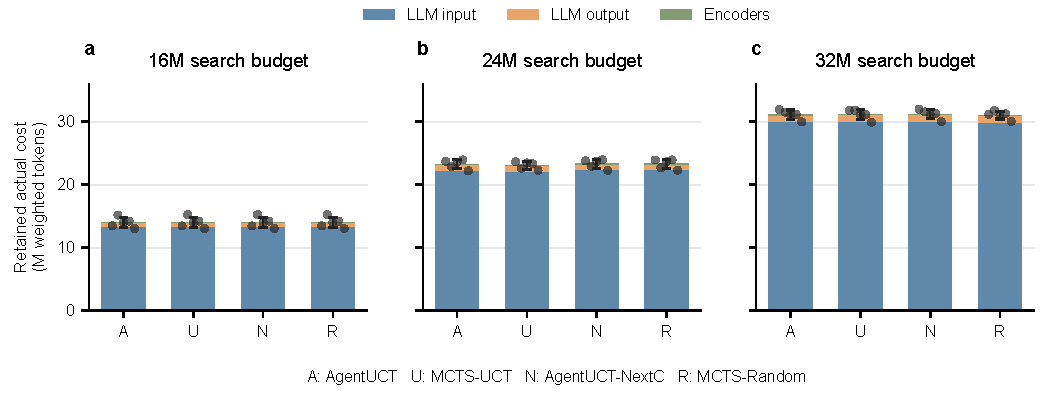
\includegraphics[width=\linewidth]{figures/rag-extended-analysis-20261004/cost-cache/retained-token-cost.pdf}
\caption{Physical composition of each retained search bill. Bars show five-seed
means, dots show each seed's total, and whiskers show sample SD of the total.
The encoder contribution is small on this common scale and is resolved in
Table~\ref{tab:raw-model-tokens}. Complete crossing and held-out bills are excluded
from these bars and reported separately.}
\label{fig:resource-composition}
\end{figure}

\paragraph{Bipartite inventory and logical reuse.}
A saved key is a pair consisting of a query identifier and its complete
execution prefix. We counted these objects from completed-prefix records,
without instantiating an earlier cache or consulting keys introduced by later
search or held-out evaluation. The 32M inventories also matched the saved
materialized inventories. For this fixed full-panel design, every successful
prefix covers all 150 queries, so adjacency density over the materialized
prefix set is one at every measured cutoff. This is not density over all
legal prefixes in the grammar. This is the rectangular special case of the
information analysis, not an empirical efficiency advantage of a denser graph.

The logical hit fraction is the sum of recorded restored-prefix edges divided
by the sum of all workflow-prefix visits across complete question evaluations.
It includes zero-token control and ordering edges; it is not hits divided by
physical LLM calls. At 32M, AgentUCT, MCTS-UCT, AgentUCT-NextC and MCTS-Random have mean
logical hit fractions of 6.79\%, 6.81\%, 6.27\% and 7.04\%, respectively
(Table~\ref{tab:cache-efficiency}). AgentUCT's 0.51-point increase over
AgentUCT-NextC accompanies only 0.183\% fewer raw LLM tokens in retained search.
Its LLM tokens per complete evaluation are higher than MCTS-UCT's (421.7k versus
418.1k). Differences in the selected workflow mix affect both quantities.
Without a matched no-cache execution, these observations do not estimate
avoided tokens or wall-clock speedup (Figure~\ref{fig:cache-work}).

\begin{table}[htbp]
\centering\small\setlength{\tabcolsep}{3pt}
\caption{Cache inventory and observed work, mean $\pm$ sample SD over five seeds.
Keys are distinct query--prefix pairs, Prefixes counts distinct full prefixes,
and Visits counts logical prefix accesses. Hit is a per-run ratio averaged
across seeds. LLM/eval is actual input plus output tokens per complete
150-question evaluation. Densities over the observed prefix sets are one.}
\label{tab:cache-efficiency}
% Actual saved receipts; mean +/- sample SD over five seeds.
\begin{tabular}{@{}llrrrrr@{}}
\toprule
$B$ (M) & Method & Keys (k) & Prefixes & Visits (k) & Hit (\%) & LLM/eval (k) \\
\midrule
16 & AgentUCT & $11.01 \pm 1.36$ & $73.4 \pm 9.0$ & $11.07 \pm 1.48$ & $0.44 \pm 0.99$ & $408.3 \pm 45.9$ \\
16 & MCTS-UCT & $11.01 \pm 1.36$ & $73.4 \pm 9.0$ & $11.07 \pm 1.48$ & $0.44 \pm 0.99$ & $408.6 \pm 45.6$ \\
16 & AgentUCT-NextC & $11.01 \pm 1.36$ & $73.4 \pm 9.0$ & $11.07 \pm 1.48$ & $0.44 \pm 0.99$ & $408.6 \pm 45.6$ \\
16 & MCTS-Random & $11.01 \pm 1.36$ & $73.4 \pm 9.0$ & $11.07 \pm 1.48$ & $0.44 \pm 0.99$ & $408.6 \pm 45.6$ \\
24 & AgentUCT & $17.19 \pm 1.86$ & $114.6 \pm 12.4$ & $18.09 \pm 2.05$ & $4.92 \pm 1.36$ & $415.6 \pm 43.5$ \\
24 & MCTS-UCT & $16.95 \pm 1.80$ & $113.0 \pm 12.0$ & $17.82 \pm 2.00$ & $4.82 \pm 1.09$ & $418.5 \pm 45.3$ \\
24 & AgentUCT-NextC & $17.28 \pm 1.82$ & $115.2 \pm 12.1$ & $18.09 \pm 2.05$ & $4.40 \pm 0.83$ & $416.6 \pm 43.8$ \\
24 & MCTS-Random & $17.34 \pm 1.79$ & $115.6 \pm 11.9$ & $18.36 \pm 2.05$ & $5.45 \pm 2.07$ & $410.0 \pm 44.6$ \\
32 & AgentUCT & $22.14 \pm 1.82$ & $147.6 \pm 12.1$ & $23.76 \pm 2.05$ & $6.79 \pm 0.82$ & $421.7 \pm 30.9$ \\
32 & MCTS-UCT & $22.38 \pm 2.14$ & $149.2 \pm 14.2$ & $24.03 \pm 2.41$ & $6.81 \pm 1.23$ & $418.1 \pm 34.8$ \\
32 & AgentUCT-NextC & $22.26 \pm 1.80$ & $148.4 \pm 12.0$ & $23.76 \pm 2.05$ & $6.27 \pm 0.66$ & $422.5 \pm 30.9$ \\
32 & MCTS-Random & $22.32 \pm 2.05$ & $148.8 \pm 13.7$ & $24.03 \pm 2.41$ & $7.04 \pm 1.56$ & $416.7 \pm 36.0$ \\
\bottomrule
\end{tabular}

\end{table}
\begin{figure}[htbp]
\centering
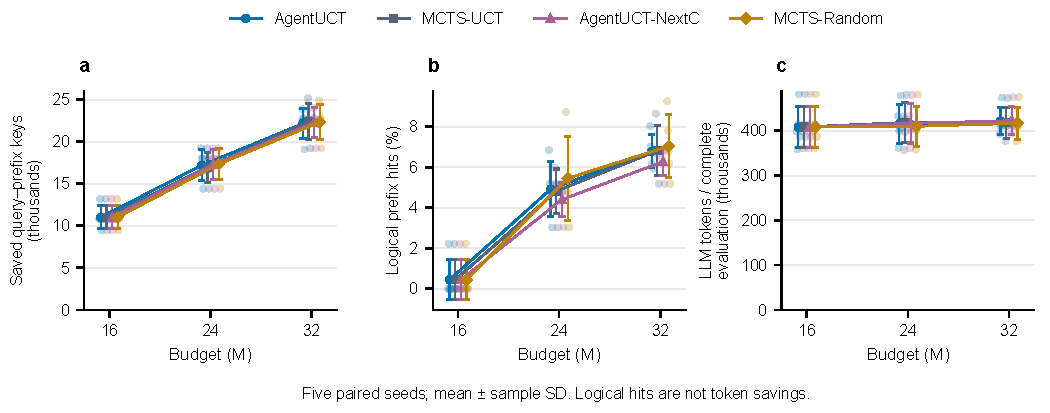
\includegraphics[width=\linewidth]{figures/rag-extended-analysis-20261004/cost-cache/cache-and-llm-work.pdf}
\caption{Saved objects, observed logical reuse and actual LLM work have different
interpretations. Markers/lines show means, whiskers show sample SD, and faint
points show the five seeds. Horizontal offsets separate methods at the same
budget; they are not different budgets. A lower SD whisker can extend below
zero because SD describes spread rather than a probability interval. Cache
hits are not a measured counterfactual saving.}
\label{fig:cache-work}
\end{figure}

\ifdefined\AgentUCTReading\else\clearpage\fi
\subsection{Execution variation and trace coverage}
Fresh executions can differ numerically. Across three shared initialization
paths and 450 question evaluations per method, MCTS-UCT differed from AgentUCT on
four answers, two affecting F1; AgentUCT-NextC and MCTS-Random matched AgentUCT.
The largest panel-mean difference was $9.52\times10^{-4}$, with identical
recorded batch prompts and query order at the differing answer. Within one
run, a successful terminal checkpoint supplies its saved prediction; the
sampled main trajectories contained no repeated complete terminal.
The quality-regret theorem assumes a fixed evaluator table, whereas these
empirical comparisons retain observed variation between fresh executions.
After the initial stage, an observer-copy repair and a retrieval-service
memory reservation optimization were deployed with separate provenance.
Fixed-request checks preserved rankings and token charges, without establishing
global bitwise equivalence across fresh runs.

The implementation must pass evidence-order, query-history, stopping,
checkpoint-restoration, physical-price update and recovery regressions.
Model-attempt records retain checkpoint, prompt, output, input/output
tokens and available timing/failure metadata. Semantic role labels were absent
from the original receipts, as noted above. Candidate traces retain raw backup statistics,
probabilities, current cost forecasts and selected actions. Search and tiny
queues perform no trace-reconstruction audit. Offline audits check saved
candidate arithmetic, backup, predictions, checkpoints and bills directly;
they do not rerun search, random draws, historical forecasts or generation.
Prediction calibration requires separate evidence. The runtime journal persists
physical receipts and completed items; the post-hoc accounting path does not
scan all earlier response bodies before a component call. Four query workers
process fixed consecutive QID groups inside one candidate. Before each model
dispatch, every unfinished group member either requests generation or finishes;
requests with equal output limits are batched in stable QID order. Cached or
failed items leave the group explicitly, and all submitted work drains before
an error propagates. Provider observers and receipts are per-query; retrieval
cache reset and ranking are atomic. All 150 training items settle before
scoring, price updates and the next search decision.
Call elapsed times may include component queueing; queue time and component
execution time are separately recorded, and their sums are not wall-clock time. Top-$m$ selection precedes
CPU ordering; ordering preserves selected text, and the final answer stage
generates the workflow's answer.

Runtime diagnostics count each physical generation batch once, using its
session and batch identifiers. Padding efficiency is the ratio of actual
tokens to padded tensor positions, reported separately for inputs and outputs.
Batch timings from a recent receipt window diagnose execution overhead;
end-to-end speed comparisons require completed, matched workloads.

New and resumed follow-up RAG runs reuse the native checkpoint already read
when a new prefix completes, removing a second checkpoint read and graph
compilation. Cache hits and process recovery still read durable checkpoints.
The saved runtime record identifies the implementation used for each launch;
search settings, fixed batches, checkpoints and actual bills are preserved.

Earlier multi-round runs remain archived diagnostics. Independent calibration
of that source pool used 34 fixed paths on three separate questions, producing
102 evaluations, 933 component receipts and 383 Qwen generation attempts.
The shared calibration bill was 1,171,878.42 weighted-token units:
1,165,642.43 for execution and 6,235.99 for index preparation. Its recorded
425.44 seconds include preparation and output persistence and exclude model
loading. The main grammar retains the
corresponding query/retrieval/reranking forecasts and transfers the former
width-conditioned answer prices to explicit final-answer edges. Removed
compression actions receive no mass in the new completion law. These transferred
price priors and the common numeric scale remain fixed across methods and tiny;
they are not calibrated error bounds. Main-runtime acceptance additionally
checks the complete one-tree, raw-backup, cache and Top-5 protocol, as well as
complete token/time records on the new trajectories.
The frozen parser accepts a singular \texttt{citation} key as an alias for
\texttt{citations} and closes one missing final object brace only when the
result is otherwise valid JSON. It still validates citation identifiers and
rejects unfinished strings or arrays. Raw output and each normalization are
retained. The revised calibration has no query fallback.

\subsection{Exploratory dynamic AFlow pilot}
The completed GSM8K pilot uses LLM-generated Python edits. Two arms pair seed 11: a bounded adaptation of AFlow's
original allocator and a dynamic-edit adaptation of AgentUCT. Both use
Qwen3.5-4B, the upstream proposal template with its XML output contract,
the actual operator interfaces and the official scorer. Each workflow is
evaluated on eight training questions before a tree update. The two best
distinct training workflows enter an eight-question validation panel; its
winner is measured on 24 primary questions, excluding one separate sentinel.
The panels are disjoint, but were previously sampled for development.

The single reporting budget is 100k raw input-plus-output tokens, with caps
of 32 complete workflows and 32 proposal rounds, each allowing up to three
proposal or repair attempts. Complete evaluations can cross the budget;
the reported snapshot is the last affordable complete state. The full bill
retains that crossing, proposals, repairs, validation and paid failures.
Test costs are separate. The diagnostic utility is
$J_{\mathrm{pilot}}=F-0.05C_{\mathrm{opt,full}}/8192$.
The inherited diagnostic scale and $\beta=2$ are not independently calibrated;
this utility is not pooled with RAG's parameter-weighted-token utility.

AFlow samples eligible top-four parents with probabilities
$0.3/K+0.7\,\mathrm{softmax}(20s)_i$. AgentUCT uses progressive widening,
raw descendant-return backup and a prequential estimate of complete edit
cost from earlier completed training proposals, repairs and executions.
The widening limit is $\min(8,\max(1,\lceil\sqrt{N}\rceil))$, with maximum
edit depth 12, exploration coefficient 1.4 and no rollout. Proposals use
temperature 0.7 and top-$p=0.9$; execution is greedy. The context cap is 8192
tokens, with output caps of 2048 for proposals and 1024 for execution.
Each question--workflow execution permits ten model-request slots, counting
retries and cache replays. Each formatted-model invocation permits up to three
format attempts within that limit; an operator can make several such invocations.
A 600-second deadline is checked between requests. An in-flight synchronous
model call settles before timeout handling, so this is not a hard wall-time cap.
Completed pilot receipts cover 276 physical calls and 251 native WTB result
checkpoints. A generated Programmer workflow executed Python on all eight
training questions. Neither arm recorded a model-response cache hit, so this
pilot does not measure reuse gains. Both selected the initial workflow.
The parent eligibility, single training evaluation, bounded repair,
feedback and program deduplication differ from upstream AFlow. The comparison
therefore tests these bounded policy adaptations, not a complete upstream
reproduction or the cost term alone. Generated code has unknown future demand;
the estimator supplies no calibrated error bound. The finite-terminal quality
theorem does not automatically apply to evaluable and expandable programs.

Each arm owns its execution cache and ledger. Python reruns while WTB restores
saved model responses at matching complete invocation prefixes. Successful
edits, adaptive selections, actual Programmer execution, failures, the full bill
and validation-to-test selection have been audited in the completed pilot.
No prefix cache hits occurred, so the observed run supplies no reuse-benefit evidence.

\subsection{AgentUCT-StaticFull ablation and selection depth}
\label{sec:static-complete-design}
AgentUCT-StaticFull is the static complete-cost ablation of AgentUCT.
It tests whether dynamic adaptation improves on a fixed complete-cost prior. Before its search begins, independent calibration fixes
the same resource-price priors and caps as AgentUCT, giving prices $\bar w_r$.
Any estimator overhead $\bar h(p,a)$ is fixed at its pre-search value.
The continuation law
$\bar\rho(\cdot\mid p,a)$ is the original estimator's zero-history law:
each successive legal child is equally likely, which does not generally
make complete terminals equally likely. The original 16 completion samples
and smoothing are retained. A private seed--state--action random tape fixes
the sampled completions without advancing search randomness. The frozen target is
\[
 \bar b(p,a)=\mathbb E_{X\sim\bar\rho(\cdot\mid p,a)}
                 \left[\sum_{r\in\mathcal D(X)}\bar w_r\right]+\bar h(p,a),
\]
and is estimated by the fixed mean of 16 sampled completions, using an empty
workflow-execution cache as the reference. Structural
zero-cost steps remain free. Shared preparation retains its original separate
account. Prices, continuation probabilities and the sampled completions for
each state--action remain fixed; the estimator reads neither live cache
membership nor later execution observations. Previously unseen states are
priced lazily from these frozen inputs, without tree enumeration, historical
reconstruction or consumption of the search random stream.

Execution still restores and extends the actual WTB cache. Raw F1 backup,
initialization, exploration, rollout, $\beta$, $C_{\rm ref}$, models, panels,
physical batching and Top5--validation--test selection match AgentUCT. Five
additional static-control searches use seeds 11, 23, 37, 53 and 71 and report
the same 16M, 24M and 32M actual-cost cutoffs. Only the price used in selection
is held static; actual failure, retry and crossing charges remain billed.
This intervention evaluates dynamic cache conditioning, price learning and
continuation adaptation jointly. It does not distinguish their individual
effects. Across all five paired seeds, AgentUCT reaches $69.57\pm0.28\%$
at both 24M and 32M, compared with $67.36\pm2.67\%$ for AgentUCT-StaticFull.
The paired difference is $2.21\pm2.89$ percentage points, with a median of
0.94 points. Seeds 37, 53 and 71 improve by 0.94, 6.76 and 3.35 points;
seeds 11 and 23 tie. All five 16M endpoints tie. At 32M, each pair retains
the same evaluation count (Table~\ref{tab:completed-static-full-paired}).
The selected workflows differ in all three seeds that improve. At 24M,
seed 53 retains fourteen dynamic evaluations versus thirteen static ones;
the other pairs have equal counts. The 24M and 32M endpoints repeat within
every seed and supply the same five paired quality comparisons.

Seeds 11 and 23 select the same configurations under both estimators: C17 at
every cutoff for seed 11, and C18/C01/C01 for seed 23. In seed 37, the dynamic
method selects C10 at 24M and 32M; the static method selects query decomposition,
\texttt{retriever.rrf}, MMR with $\lambda=0.3$, ten retrieved documents, one
retrieval pass, identity reranking, four documents in ranked order and
\texttt{answer.generate:m=4}. In seed 53, the static method retains C03 at
every cutoff, whereas dynamic pricing selects C15 at 24M and 32M.
Seed 71 selects C05 under both methods at 16M. At 24M and 32M the dynamic
method selects C19; the static method selects query decomposition, weighted
BM25--Qwen retrieval with BM25 weight 0.75, MMR with $\lambda=0.3$, ten
retrieved documents, one retrieval pass, Qwen reranking, two documents in
ranked order and \texttt{answer.generate:m=2}. The static seed-37 and seed-71
recipes are written explicitly because they have no identifier in the
original configuration catalogue.

\begin{table*}[t]
\centering\small
\caption{Completed paired seeds for the AgentUCT-StaticFull ablation. Test F1 is
in percent and is directly compared across methods;
$N_{\rm dyn}$/$N_{\rm stat}$ count affordable complete evaluations. Both
methods use the live execution cache; only the selection-cost estimator is
frozen in AgentUCT-StaticFull. Reused endpoints across cutoffs are correlated
measurements, not additional independent trials. All five planned paired
seeds are complete.}
\label{tab:completed-static-full-paired}
\begin{tabular}{@{}rrrrrr@{}}
\toprule
Seed & $B$ (M) & AgentUCT & \shortstack{AgentUCT-\\StaticFull} & $N_{\rm dyn}$ & $N_{\rm stat}$\\
\midrule
11 & 16 & 69.51 & 69.51 & 8 & 8\\
11 & 24 & 69.51 & 69.51 & 13 & 13\\
11 & 32 & 69.51 & 69.51 & 18 & 18\\
23 & 16 & 67.05 & 67.05 & 10 & 10\\
23 & 24 & 69.52 & 69.52 & 15 & 15\\
23 & 32 & 69.52 & 69.52 & 19 & 19\\
37 & 16 & 69.20 & 69.20 & 8 & 8\\
37 & 24 & 69.20 & 68.26 & 14 & 14\\
37 & 32 & 69.20 & 68.26 & 18 & 18\\
53 & 16 & 63.21 & 63.21 & 7 & 7\\
53 & 24 & 69.97 & 63.21 & 14 & 13\\
53 & 32 & 69.97 & 63.21 & 18 & 18\\
71 & 16 & 68.01 & 68.01 & 8 & 8\\
71 & 24 & 69.63 & 66.28 & 11 & 11\\
71 & 32 & 69.63 & 66.28 & 15 & 15\\
\bottomrule
\end{tabular}

\end{table*}

Table~\ref{tab:static-full-phase-bills} records the complete physical bill for
each static-control run. Whole crossing evaluations remain charged; the
amount exceeding 32M is only part of that work. Validation and test columns
cover the requested cutoff measurements at all three budgets, with complete
measurements reused when endpoints repeat. Previously paid input preparation
is referenced separately and is not charged again as new work.

\begin{table*}[t]
\centering\small\setlength{\tabcolsep}{4pt}
\caption{AgentUCT-StaticFull phase bills in M weighted-token units. Full search
includes the entire crossing evaluation; retained cost excludes it from the
32M snapshot. Overshoot is full search minus 32M. Validation and test include
the three-cutoff measurement campaign. Paid input preparation is a reference
to prior physical work, not a new zero-cost preparation claim.}
\label{tab:static-full-phase-bills}
\begin{tabular}{@{}rrrrrrrr@{}}
\toprule
Seed & Full search & Retained 32M & Crossing & Overshoot & Validation & Test & Paid input prep.\\
\midrule
11 & 33.693 & 31.982 & 1.711 & 1.693 & 39.807 & 3.641 & 1.792\\
23 & 32.201 & 31.481 & 0.720 & 0.201 & 36.067 & 8.222 & 1.792\\
37 & 32.210 & 30.985 & 1.224 & 0.210 & 35.786 & 12.124 & 1.792\\
53 & 33.851 & 31.277 & 2.574 & 1.851 & 33.264 & 8.372 & 1.792\\
71 & 32.218 & 29.949 & 2.269 & 0.218 & 49.845 & 15.719 & 1.792\\
\bottomrule
\end{tabular}

\end{table*}

The implementation retains the original zero-history sampling tape and
prices the entire root-to-terminal evaluation, including its selected tree
prefix, against the empty cache. Static observation hooks skip receipt-based
price and transition updates; the execution ledger still records every actual
call. A separate run namespace preserves the original dynamic-control results.

The saved RAG evidence in Table~\ref{tab:initialization-paired-evidence}
connects initialization cost, first complete adaptive feedback, cost-induced
selection changes and paired endpoint effects. In the diagnostic GSM8K
seed-11 trace, completion pricing also changed a decision below the root.
Through nineteen completed AgentUCT training panels, twenty-one recorded
traversal decisions included eight below the root, two at selection-state
depth two. The cost term changed seventeen choices overall, including five
below the root. MCTS-UCT completed nineteen panels and recorded seventeen
traversal decisions, four below the root. These traces establish recursive
allocation, without establishing an endpoint-quality benefit.

Search in this execution cohort terminated before its first reporting budget.
Repeated per-question errors inflated the proposal history beyond the fixed
6,144-token input allowance; repeated context rejections then exhausted the
256-proposal limit. AFlow, MCTS-UCT and AgentUCT completed 20, 19 and 19 training
panels at 4.504M, 5.891M and 5.818M raw search tokens, respectively, all below
6.423M. These runs are diagnostic evidence, not completed target-budget trials.
A separate common cohort encodes identical errors and consecutive identical
unevaluated failures with their occurrence counts. It retains every distinct
error and evaluated sibling, the complete task and parent program, and the
original context limit, model, data, budgets and allocation rules. This change
alters proposal inputs and therefore requires fresh runs for all three methods;
old and new measurements are not pooled.

The replacement seed-11 cohort recorded recursive allocation through deeper
selection states. The full AgentUCT search, including its crossing evaluation,
completed 92 training panels and recorded 210 traversal decisions, including
127 below the root, reaching selection-state depth four. Completion pricing
changed 185 decisions, including 107 below the root. The retained 19.122M
snapshot ended at iteration 90: its 91 panels contained 207 traversal
decisions, 125 below the root, with 182 cost-induced changes, 105 below the
root. The full MCTS-UCT search completed 60 panels and recorded 79 traversal
decisions, 28 below the root, reaching selection-state depth one. Its 19.122M
snapshot ended at iteration 58 and contained 77 traversal decisions,
27 below the root. All MCTS-UCT choices matched the cost-free index.
AFlow completed 89 panels. Generated-program errors remained scored and billed.

At the 19.122M budget, AgentUCT answered one more test question correctly
than MCTS-UCT in seed 11 (279 versus 278 of 300), a difference of one-third
of a percentage point (Table~\ref{tab:gsm-counted-seed11}). AFlow scored
95\%, two percentage points above AgentUCT's 93\%, and was highest in this
seed. This single paired seed does not establish across-seed performance
or a quality benefit from deeper allocation.
AgentUCT, MCTS-UCT and AFlow used nine, seven and eight distinct validation
measurements, respectively, and two distinct test measurements each.
AgentUCT's first two budgets selected node 11 and reused the same test.
The last two budgets for MCTS-UCT and AFlow likewise reused tests of
nodes 34 and 36, respectively. These repeated endpoints are not independent
replicates.

\begin{table}[t]
\centering\small
\caption{Completed GSM8K results for seed 11 in the replacement cohort.
Each row retains the last complete search checkpoint within budget; $N$
counts 150-question training panels. Correct answers and test accuracy use
300 primary questions after Top5$\to$validation selection. Costs are millions
of raw tokens. These measurements cover one paired seed.}
\label{tab:gsm-counted-seed11}
\setlength{\tabcolsep}{4pt}
\begin{tabular}{@{}lrrrrr@{}}
\toprule
Method & Budget (M) & $N$ & Retained (M) & Correct / 300 & Test acc. (\%)\\
\midrule
AgentUCT & 6.423 & 33 & 6.378792 & 278 & 92.67\\
AgentUCT & 12.772 & 60 & 12.402108 & 278 & 92.67\\
AgentUCT & 19.122 & 91 & 18.863808 & 279 & 93.00\\
\midrule
MCTS-UCT & 6.423 & 30 & 5.982823 & 279 & 93.00\\
MCTS-UCT & 12.772 & 51 & 12.112399 & 278 & 92.67\\
MCTS-UCT & 19.122 & 59 & 18.513759 & 278 & 92.67\\
\midrule
AFlow & 6.423 & 24 & 5.994099 & 279 & 93.00\\
AFlow & 12.772 & 56 & 12.550687 & 285 & 95.00\\
AFlow & 19.122 & 88 & 19.120109 & 285 & 95.00\\
\bottomrule
\end{tabular}
\end{table}

The complete MCTS-UCT bill was 25.474833M raw tokens: 20.704149M for search,
3.772249M for validation and 0.998435M for testing. Its search bill included
0.208821M for proposals and 0.131491M for repairs.
The complete AgentUCT bill was 23.647388M: 19.432714M for search,
3.216239M for validation and 0.998435M for testing. Its search bill included
0.305519M for proposals and 0.240910M for repairs. The complete AFlow bill
was 24.428076M: 19.297776M for search, 3.333025M for validation and 1.797275M
for testing, with 0.317823M for proposals and 0.212644M for repairs included
in search. At the largest budget, the final search increments through
complete evaluations cost 2.190390M for MCTS-UCT, 0.568906M for AgentUCT
and 0.177667M for AFlow. Their respective search-budget overshoots were
1.582149M, 0.310714M and 0.175776M.
These full increments remain billed; their rewards and states are excluded
from the affordable snapshots.

For seed 53, AgentUCT selected node 17 at all three reporting budgets
and obtained 277/300 correct answers (Table~\ref{tab:gsm-counted-aflow-seed53}).
The repeated endpoint reuses one complete test measurement. AFlow selected
nodes 5, 10 and 43 with separate test measurements; its accuracy decreased
from 93\% to 92\% as the budget increased. The complete matched MCTS-UCT and five-seed results are reported in
Table~\ref{tab:gsm-counted-all-five-seed}.

\begin{table}[t]
\centering\small
\caption{Completed AgentUCT and AFlow GSM8K results for seed 53 in the
replacement cohort. Each budget uses its last affordable complete checkpoint
and Top5$\to$validation selection. $N$ counts 150-question training panels;
accuracy uses the same 300 primary test questions. Costs are M raw tokens.
The three AgentUCT rows reuse one test measurement.}
\label{tab:gsm-counted-aflow-seed53}
\setlength{\tabcolsep}{4pt}
\begin{tabular}{@{}lrrrrr@{}}
\toprule
Method & Budget (M) & $N$ & Retained (M) & Correct / 300 & Test acc. (\%)\\
\midrule
AgentUCT & 6.423 & 24 & 6.274982 & 277 & 92.33\\
AgentUCT & 12.772 & 48 & 12.674662 & 277 & 92.33\\
AgentUCT & 19.122 & 99 & 18.640472 & 277 & 92.33\\
AFlow & 6.423 & 18 & 6.155695 & 279 & 93.00\\
AFlow & 12.772 & 35 & 12.543798 & 277 & 92.33\\
AFlow & 19.122 & 48 & 19.011865 & 276 & 92.00\\
\bottomrule
\end{tabular}
\end{table}

The complete seed-53 AgentUCT search evaluated 100 training panels and used
10 distinct validation panels and one test measurement. Its 23.929074M
raw-token bill comprised 19.252406M for search, 4.307082M for validation
and 0.369586M for testing. All 39,624 physical calls were settled, with no
physical call failures; 2,461 question executions with candidate-program
errors remained scored and billed. The last complete crossing evaluation
cost 0.611934M, whereas the search-budget overshoot was 0.130406M.
The crossing charges remain in the full bill, and future rewards and states
are excluded from earlier affordable snapshots.

The complete seed-53 AFlow search evaluated 49 training panels and used
11 distinct validation and three test measurements. Its 27.464199M raw-token
bill comprised 19.799962M for search, 5.391294M for validation and 2.272943M
for testing. Search included 0.232454M for proposals and 0.316211M for
repairs. All 29,115 physical calls were settled, including three failed
calls; 877 question executions with candidate-program errors remained
scored and billed. The last complete crossing evaluation cost 0.788097M,
whereas the amount above the 19.122M budget was 0.677962M. The former
remains in the full bill and is excluded from the retained snapshot.

The completed AFlow runs for seeds 23 and 71 improved from the first
to the second reporting budget, then reused their selected workflows at
the largest budget (Table~\ref{tab:gsm-counted-aflow-seeds23-71}).
Seed 23 selected nodes 18, 67 and 67; seed 71 selected nodes 0, 40 and 40.
For each seed, the last two budgets therefore share one complete test
measurement. All budgets use the same 300 primary questions, so these
measurements provide correlated endpoints. The complete AgentUCT and MCTS-UCT cohorts are included in
Table~\ref{tab:gsm-counted-all-five-seed}; the seed-23 comparison follows below.

\begin{table}[t]
\centering\small
\caption{Completed AFlow GSM8K results for seeds 23 and 71 in the
replacement cohort. Budgets retain the last affordable complete checkpoint
and use Top5$\to$validation selection. $N$ counts complete 150-question
training panels; accuracy uses 300 primary test questions. Costs are M raw
tokens. Each seed's last two rows reuse one test measurement.}
\label{tab:gsm-counted-aflow-seeds23-71}
\setlength{\tabcolsep}{4pt}
\begin{tabular}{@{}rrrrrr@{}}
\toprule
Seed & Budget (M) & $N$ & Retained (M) & Correct / 300 & Test acc. (\%)\\
\midrule
23 & 6.423 & 43 & 6.366318 & 265 & 88.33\\
23 & 12.772 & 77 & 12.478360 & 278 & 92.67\\
23 & 19.122 & 104 & 18.579361 & 278 & 92.67\\
71 & 6.423 & 24 & 6.314414 & 274 & 91.33\\
71 & 12.772 & 41 & 12.520418 & 275 & 91.67\\
71 & 19.122 & 66 & 18.914536 & 275 & 91.67\\
\bottomrule
\end{tabular}
\end{table}

The full seed-23 bill was 24.803149M raw tokens: 19.610508M for search,
3.514002M for validation and 1.678639M for testing. Search included
0.555961M for proposals and 0.557993M for repairs. Its 105 training panels,
10 distinct validation panels and two test measurements contained 19,352
official question scores. All 25,171 physical calls were settled, including
five failed calls; 1,577 question executions with candidate-program errors
remained scored and billed. The last complete crossing evaluation cost
1.031147M, with a search-budget overshoot of 0.488508M.

For seed 71, the corresponding full bill was 25.375785M: 19.515219M for
search, 5.260455M for validation and 0.600111M for testing. Search included
0.283484M for proposals and 0.212275M for repairs. Its 67 training panels,
12 distinct validation panels and two test measurements contained 14,252
official question scores. All 26,705 physical calls were settled, including
129 failed calls; 1,047 question executions with candidate-program errors
remained scored and billed. The final complete crossing cost 0.600683M,
with a search-budget overshoot of 0.393219M. Both runs retain these crossing
charges in their full bills and exclude future rewards and states from
earlier affordable snapshots.

AgentUCT and MCTS-UCT seed 23 each reused one selected workflow across
all three budgets (Table~\ref{tab:gsm-counted-agentuct-seed23}). AgentUCT
selected node 18 and answered 286/300 questions correctly (95.33\%);
MCTS-UCT selected node 13 and answered 282/300 (94.00\%). The completed
AFlow seed-23 accuracies were 88.33\%, 92.67\% and 92.67\% at the respective
budgets. These results describe one matched three-method seed; repeated
budget endpoints are correlated. The full five-seed comparison is reported
in Table~\ref{tab:gsm-counted-all-five-seed}.

\begin{table}[t]
\centering\small
\caption{Completed AgentUCT and MCTS-UCT GSM8K seed 23. Each budget retains
the last affordable complete checkpoint and uses Top5$\to$validation selection.
$N$ counts 150-question training panels; accuracy uses the same 300 primary
test questions. AgentUCT reuses node 18's one test measurement, and MCTS-UCT
reuses node 13's one test measurement. Costs are M raw tokens.}
\label{tab:gsm-counted-agentuct-seed23}
\setlength{\tabcolsep}{4pt}
\begin{tabular}{@{}lrrrrr@{}}
\toprule
Method & Budget (M) & $N$ & Retained (M) & Correct / 300 & Test acc. (\%)\\
\midrule
AgentUCT & 6.423 & 34 & 6.303265 & 286 & 95.33\\
AgentUCT & 12.772 & 78 & 12.752482 & 286 & 95.33\\
AgentUCT & 19.122 & 123 & 18.919751 & 286 & 95.33\\
MCTS-UCT & 6.423 & 36 & 6.401393 & 282 & 94.00\\
MCTS-UCT & 12.772 & 72 & 11.131243 & 282 & 94.00\\
MCTS-UCT & 19.122 & 95 & 18.979224 & 282 & 94.00\\
\bottomrule
\end{tabular}
\end{table}

The full seed-23 AgentUCT bill was 23.894398M raw tokens: 19.231072M
for search, 4.033069M for validation and 0.630257M for testing. Search
included 0.452297M for proposals and 0.417624M for repairs. Its 124
training panels, eight distinct validation panels and one test measurement
retained all 32,151 settled physical calls, with no physical call failures;
2,190 question executions with candidate-program errors remained scored
and billed. The last complete crossing evaluation cost 0.311321M,
whereas the search-budget overshoot was 0.109072M. The full bill retains
crossing charges, and earlier snapshots exclude future rewards and states.
The original preparation remains separate.

% Sources: gsm-counted-uct-seed23-completion-audit.json and
% gsm-counted-uct-seed23-independent-review-20261007.json.
The full seed-23 MCTS-UCT bill was 22.407630M raw tokens: 19.348587M
for search, 2.195358M for validation and 0.863685M for testing. Search
included 18.776162M for workflow execution, 0.313854M for proposals and
0.258571M for repairs. Its 96 training panels, five distinct validation
panels and one test measurement covered 16,201 question executions,
including one diagnostic test sentinel excluded from primary accuracy.
All 24,844 physical calls settled, including three failed calls; 2,083
question executions with workflow errors remained scored and billed.
The last complete crossing evaluation cost 0.369363M, whereas the
search-budget overshoot was 0.226587M. The complete crossing charge
remains in the full bill; earlier affordable snapshots exclude future
rewards and states. The
shared preparation of 0.109983M raw tokens remains separate.

For seed 37, AgentUCT obtained 281, 280 and 280 correct answers across
the three budgets, whereas AFlow obtained 277, 279 and 282
(Table~\ref{tab:gsm-counted-seed37}). AgentUCT reused node 75 at the last
two budgets; AFlow selected nodes 50, 96 and 125 with distinct test
measurements. The ranking therefore changed with budget in this seed.
The matched MCTS-UCT results appear in the complete five-seed comparison
(Table~\ref{tab:gsm-counted-all-five-seed}).

\begin{table}[t]
\centering\small
\caption{Completed AgentUCT and AFlow GSM8K results for seed 37 in the
replacement cohort. Each budget uses the last affordable complete checkpoint
and Top5$\to$validation selection. $N$ counts 150-question training panels;
accuracy uses the same 300 primary test questions. Costs are M raw tokens.
The last two AgentUCT rows reuse one test measurement.}
\label{tab:gsm-counted-seed37}
\setlength{\tabcolsep}{4pt}
\begin{tabular}{@{}lrrrrr@{}}
\toprule
Method & Budget (M) & $N$ & Retained (M) & Correct / 300 & Test acc. (\%)\\
\midrule
AgentUCT & 6.423 & 50 & 6.388173 & 281 & 93.67\\
AgentUCT & 12.772 & 76 & 12.763173 & 280 & 93.33\\
AgentUCT & 19.122 & 116 & 18.959821 & 280 & 93.33\\
AFlow & 6.423 & 52 & 6.362538 & 277 & 92.33\\
AFlow & 12.772 & 98 & 12.732002 & 279 & 93.00\\
AFlow & 19.122 & 159 & 19.102452 & 282 & 94.00\\
\bottomrule
\end{tabular}
\end{table}

The full seed-37 AgentUCT bill was 20.506717M raw tokens: 19.216682M
for search, 0.905446M for validation and 0.384589M for testing. Search
included 0.440943M for proposals and 0.399368M for repairs. Its 117
training panels, seven distinct validation panels and two test measurements
retained all 22,142 settled physical calls, with no physical call failures;
3,019 question executions with candidate-program errors remained scored
and billed. The last complete crossing evaluation cost 0.256861M,
whereas the search-budget overshoot was 0.094682M.

For AFlow seed 37, the full bill was 20.307432M: 19.123214M for search,
0.701023M for validation and 0.483195M for testing. Search included
0.804010M for proposals and 0.629095M for repairs. Its 160 training panels,
ten distinct validation panels and three test measurements retained all
26,204 settled physical calls, including four failed calls; 2,312 question
executions with candidate-program errors remained scored and billed.
The last complete crossing evaluation cost 0.020762M, whereas the
overshoot was 0.001214M. Both runs preserve these crossing charges in
their full bills and exclude future rewards and states from earlier
affordable snapshots. The original 109,983-token preparation remains
separate; neither run required new preparation or calibration.

Saved AgentUCT seed-37 traversals contain 294 parent-state choices,
186 below the root; completion pricing changes 253 choices, including
148 below the root. At the largest affordable snapshot, the corresponding
counts are 290, 183, 250 and 146. The remaining four choices belong to
the crossing evaluation and are excluded from that snapshot. The highest
saved parent depth is four in both scopes. These are recorded allocation
decisions, not program depth or a causal estimate of their quality benefit.

The AFlow arm is now complete for all five seeds
(Table~\ref{tab:gsm-counted-aflow-five-seed}). Mean accuracy rises from
$91.60\pm1.95\%$ to $93.07\pm1.40\%$ across the reporting budgets,
with a decrease for seed 53 and repeated selected endpoints in seeds 11,
23 and 71. These are within-method observations. The complete matched AgentUCT and MCTS-UCT cohorts are reported in
Table~\ref{tab:gsm-counted-all-five-seed}.

\begin{table}[t]
\centering\small
\caption{Complete AFlow GSM8K arm: original test accuracy (\%) for each
seed and mean $\pm$ sample SD across five seeds. Budget columns are M raw
search tokens and use Top5$\to$validation selection. All rows use the same
300 primary test questions; budgets are correlated and can reuse an endpoint.}
\label{tab:gsm-counted-aflow-five-seed}
\begin{tabular}{@{}lrrr@{}}
\toprule
Seed & 6.423M & 12.772M & 19.122M\\
\midrule
11 & 93.00 & 95.00 & 95.00\\
23 & 88.33 & 92.67 & 92.67\\
37 & 92.33 & 93.00 & 94.00\\
53 & 93.00 & 92.33 & 92.00\\
71 & 91.33 & 91.67 & 91.67\\
Mean $\pm$ sample SD & $91.60\pm1.95$ & $92.93\pm1.26$ & $93.07\pm1.40$\\
\bottomrule
\end{tabular}
\end{table}

Table~\ref{tab:gsm-nonroot-choice} shows the cost-induced depth-one decision.
At parent node 5, the quality-plus-exploration index favoured node 7.
Its estimated complete edit-and-evaluation cost was 1.382M raw tokens, compared with
0.249M for node 6, so AgentUCT selected node 6 as the next edit's input.
The resulting new program, node 9, scored zero on its complete 150-question
training panel. The trace therefore establishes that completion pricing
affected recursive allocation; it supplies no quality-gain evidence for this
particular choice. Candidate statistics are taken from the contemporaneous
saved traversal. Selection-state depth follows saved parent links and is
distinct from the depth of the generated program.

\begin{table}[t]
\centering
\caption{A saved depth-one AgentUCT decision in the diagnostic GSM8K
seed-11 run, edit 9. Both candidates are children of node 5. The cost-free
index selects node 7; subtracting $2\widehat b/C_{\rm ref}$ selects node 6,
with $C_{\rm ref}=150{,}954.5$ raw tokens. The edited child subsequently scored
zero on the training panel; no endpoint-quality claim follows from this case.}
\label{tab:gsm-nonroot-choice}
\small
\begin{tabular}{lrrrrrr}
\toprule
Node & $N$ & $Q$ & Bonus & $Q+\mathrm{bonus}$ & Est. cost (M) & Net index\\
\midrule
6 (selected) & 2 & 0.3067 & 1.2559 & 1.5626 & 0.2494 & $-1.7424$\\
7 & 1 & 0.2533 & 1.7761 & 2.0294 & 1.3822 & $-16.2831$\\
\bottomrule
\end{tabular}
\end{table}

\subsection{Complete five-seed generated-workflow comparison}
\label{sec:gsm-five-seed-complete}
Completion pricing produced a modest mean quality advantage over MCTS-UCT
in the frozen GSM8K AFlow system (Table~\ref{tab:gsm-counted-all-five-seed}).
At 19.122M raw search tokens, AgentUCT reached $93.07\pm1.48\%$,
compared with $92.67\pm0.78\%$ for MCTS-UCT and
$93.07\pm1.40\%$ for AFlow. AgentUCT exceeded MCTS-UCT
in seeds 11, 23 and 37, tied it in seed 53, and scored lower in seed 71.
AgentUCT and AFlow had the same largest-budget mean, despite different
seed outcomes. All three frozen budgets and all five seeds are retained;
this is a task-specific allocation comparison, not a universal ordering.
AgentUCT seed 71 selected its initial node 0 at all three budgets, reusing
one test measurement. Recorded recursive allocation changes elsewhere do not
attribute an endpoint gain to this unchanged selection.
The primary denominator is 300 test questions per endpoint; the diagnostic
sentinel is excluded. The shared Qwen3.5-4B, fixed-eight execution groups,
counted-error proposal history, complete 150-question training joins and
Top5-to-validation selection are unchanged.

\begin{table}[t]
\centering\small
\caption{Complete GSM8K comparison across 5 paired search seeds. Test accuracy (\%) is reported directly for every seed and all frozen raw-token budgets. Mean $\pm$ sample SD equally weights seeds; SD is not a confidence interval. The same test questions and repeated selected endpoints make budget columns correlated.}
\label{tab:gsm-counted-all-five-seed}
\begin{tabular}{@{}llrrr@{}}
\toprule
Method & Seed & 6.423M & 12.772M & 19.122M\\
\midrule
AgentUCT & 11 & 92.67 & 92.67 & 93.00\\
AgentUCT & 23 & 95.33 & 95.33 & 95.33\\
AgentUCT & 37 & 93.67 & 93.33 & 93.33\\
AgentUCT & 53 & 92.33 & 92.33 & 92.33\\
AgentUCT & 71 & 91.33 & 91.33 & 91.33\\
AgentUCT & Mean $\pm$ SD & $93.07\pm1.52$ & $93.00\pm1.49$ & $93.07\pm1.48$\\
\midrule
MCTS-UCT & 11 & 93.00 & 92.67 & 92.67\\
MCTS-UCT & 23 & 94.00 & 94.00 & 94.00\\
MCTS-UCT & 37 & 91.33 & 92.33 & 92.33\\
MCTS-UCT & 53 & 93.00 & 92.33 & 92.33\\
MCTS-UCT & 71 & 91.67 & 91.67 & 92.00\\
MCTS-UCT & Mean $\pm$ SD & $92.60\pm1.09$ & $92.60\pm0.86$ & $92.67\pm0.78$\\
\midrule
AFlow & 11 & 93.00 & 95.00 & 95.00\\
AFlow & 23 & 88.33 & 92.67 & 92.67\\
AFlow & 37 & 92.33 & 93.00 & 94.00\\
AFlow & 53 & 93.00 & 92.33 & 92.00\\
AFlow & 71 & 91.33 & 91.67 & 91.67\\
AFlow & Mean $\pm$ SD & $91.60\pm1.95$ & $92.93\pm1.26$ & $93.07\pm1.40$\\
\bottomrule
\end{tabular}
\end{table}
\begin{table}[t]
\centering\footnotesize
\setlength{\tabcolsep}{3pt}
\caption{Actual bills and failures for the four newly completed GSM8K units. All costs are M raw tokens. Search includes execution, proposer and repair calls. Full formal totals include all crossing evaluations, validation, testing and failures; shared preparation or calibration is separate. Overshoot is already contained in search, not an additional charge.}
\label{tab:core-new-unit-bills}
\begin{tabular}{@{}llrrrrrr@{}}
\toprule
Task & Method / seed & Search & Valid. & Test & Formal & Calls & Failed\\
\midrule
GSM8K & AgentUCT / 71 & 19.358143 & 7.312719 & 0.149341 & 26.820203 & 25794 & 0\\
GSM8K & MCTS-UCT / 37 & 20.092556 & 1.927642 & 0.403501 & 22.423699 & 27746 & 0\\
GSM8K & MCTS-UCT / 53 & 19.415722 & 2.541933 & 1.134356 & 23.092011 & 36146 & 0\\
GSM8K & MCTS-UCT / 71 & 19.168017 & 2.252405 & 0.501162 & 21.921584 & 25427 & 0\\
\bottomrule
\end{tabular}
\end{table}

For the newly completed GSM8K units, the complete training, distinct validation
and test panel counts were AgentUCT seed 71 (52/11/1), MCTS-UCT seed 37 (98/8/2), MCTS-UCT seed 53 (93/9/2), MCTS-UCT seed 71 (72/7/2).
Every physical call settled. Workflow errors remained scored and billed:
AgentUCT seed 71 (1,371 question executions), MCTS-UCT seed 37 (3,181 question executions), MCTS-UCT seed 53 (2,158 question executions), MCTS-UCT seed 71 (978 question executions).
The largest-budget complete crossing and overshoot amounts, respectively,
were AgentUCT seed 71 (0.267421M/0.236143M), MCTS-UCT seed 37 (1.227992M/0.970556M), MCTS-UCT seed 53 (0.777511M/0.293722M), MCTS-UCT seed 71 (0.100444M/0.046017M).
The overshoot is a subset of the billed crossing work. Last affordable
complete snapshots exclude its future rewards and states. Shared preparation
remains 0.109983M raw tokens.

\ifdefined\AgentUCTReading\else\clearpage\fi
\subsection{Complete training-Top1 measurements}
\label{sec:top1-complete}
The no-validation ablation covers all sixty method--seed--budget cells.
For each completed affordable search prefix, the highest training mean F1
selects the endpoint, with the earliest evaluation breaking ties. Its paired
selection effect is
\[
 \Delta_{s,B}^{\mathrm{selection}}
 =F^{\mathrm{train\ Top1}}_{s,B}-F^{\mathrm{Top5\to validation}}_{s,B}.
\]
Forty-nine cells reuse complete tests of the exact workflow from the same
original run. Eight additional method--seed workflow measurements, involving
four distinct configurations, supply the remaining eleven cells. They require
2,400 primary question--workflow executions and eight sentinels. Each
prediction was rescored with the official evaluator and bound to its saved
execution and terminal receipt. The new measurements contain 21,680 settled
component/preparation records and 5,791 generation attempts, costing 29.722M
weighted-token units in the separate ablation-test account. They add no search
observations and do not change historical snapshots.

\begin{figure*}[t]
\centering
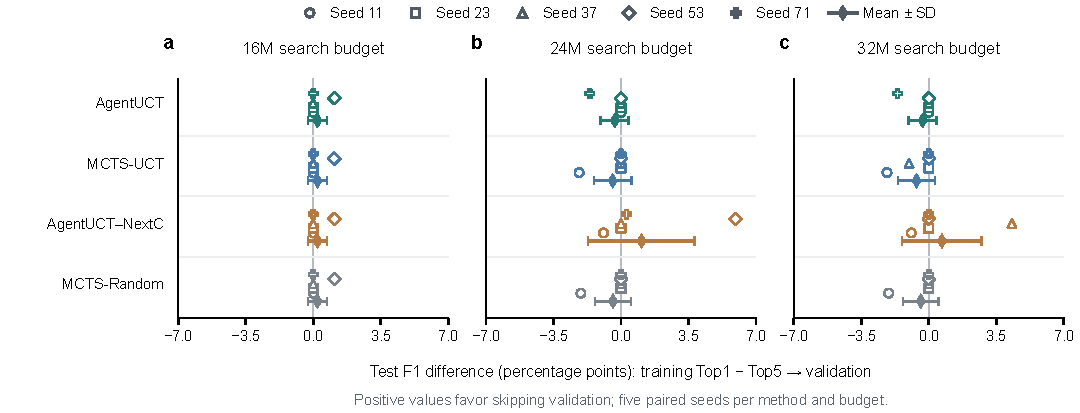
\includegraphics[width=\textwidth]{figures/top1-ablation-20261004/top1-paired-differences.pdf}
\caption{Complete effect of skipping validation. Positive paired test-F1
changes favor training Top1. Small symbols retain each seed; the lower filled
diamond and horizontal bar show mean $\pm$ sample SD across five seeds.
Both rules use the same search prefix. Repeated budgets can reuse endpoints
and are not independent replicates.}
\label{fig:top1-ablation-all}
\end{figure*}

\begin{table*}[t]
\centering\small
\caption{Complete selection ablation. Test F1 is in percent; paired
$\Delta$ is in percentage points, positive for training Top1. Scores and
differences are mean $\pm$ sample SD across five matched seeds. Win/tie/loss
compares endpoint-selection rules within a seed.}
\label{tab:top1-results}
\begin{tabular}{llcccc}
\toprule
Budget & Method & Train Top1 & Top5 $\to$ validation & Paired $\Delta$ & Win/tie/loss\\
\midrule
16M & AgentUCT & $67.61\pm2.09$ & $67.40\pm2.54$ & $+0.22\pm0.49$ & 1/4/0\\
16M & MCTS-UCT & $67.60\pm2.08$ & $67.38\pm2.52$ & $+0.22\pm0.49$ & 1/4/0\\
16M & AgentUCT--NextC & $67.61\pm2.09$ & $67.40\pm2.54$ & $+0.22\pm0.49$ & 1/4/0\\
16M & MCTS-Random & $67.61\pm2.09$ & $67.40\pm2.54$ & $+0.22\pm0.49$ & 1/4/0\\
\midrule
24M & AgentUCT & $69.24\pm0.74$ & $69.57\pm0.28$ & $-0.32\pm0.72$ & 0/4/1\\
24M & MCTS-UCT & $67.57\pm0.80$ & $68.01\pm1.12$ & $-0.43\pm0.97$ & 0/4/1\\
24M & AgentUCT--NextC & $68.90\pm0.59$ & $67.83\pm2.69$ & $+1.06\pm2.77$ & 2/2/1\\
24M & MCTS-Random & $68.02\pm0.84$ & $68.44\pm0.89$ & $-0.42\pm0.93$ & 0/4/1\\
\midrule
32M & AgentUCT & $69.24\pm0.74$ & $69.57\pm0.28$ & $-0.32\pm0.72$ & 0/4/1\\
32M & MCTS-UCT & $67.37\pm0.53$ & $68.01\pm1.12$ & $-0.64\pm0.96$ & 0/3/2\\
32M & AgentUCT--NextC & $68.90\pm0.59$ & $68.22\pm1.96$ & $+0.68\pm2.07$ & 1/3/1\\
32M & MCTS-Random & $68.38\pm1.03$ & $68.80\pm0.87$ & $-0.42\pm0.93$ & 0/4/1\\
\bottomrule
\end{tabular}

\end{table*}

At 16M, skipping validation raises all four method means by 0.22 percentage
points, entirely from seed 53. At 32M it lowers AgentUCT by 0.32 points,
MCTS-UCT by 0.64 points and MCTS-Random by 0.42 points, while raising AgentUCT-NextC by
0.68 points. Across the sixty correlated cells, seven improve and nine
decline; the other 44 select the same workflow under both rules. AgentUCT
retains the highest mean at 24M and 32M under either rule. Other method
rankings change: AgentUCT-NextC overtakes MCTS-Random at 32M and both MCTS-UCT and MCTS-Random
tree at 24M. These changes are descriptive; no test outcome changes the
primary Top5--validation protocol. Omitting validation avoids its physical
bill, while the extra test measurements remain a separate research expense.

\section{Algorithm Adapters in the Shared RAG Grammar}
\label{sec:rag-optimizer-adapters}

The direct comparison holds the executable workflow family fixed and changes
how the next evaluation is chosen. This section specifies the implemented
adapters behind Table~\ref{tab:direct-algorithm-coverage}. It documents an
experimental protocol; the pending rows have no completed five-seed quality
estimate. The original algorithms motivate the selection rules, while the
categorical representation, RAG observations and shared execution service
define their use in this study.

\subsection{Common representation, feedback and accounting}
\label{sec:adapter-common-contract}
Write a legal workflow as $x=(a_1,\ldots,a_9)$. Its actions select the query,
retriever, relevance or diversity rule, retrieval width, stopping rule,
reranker, retained evidence count, context order and answer generator.
The no-loop grammar has 61,344 terminal tuples. A candidate is legal only if
every action is admitted after its preceding prefix; this enforces the
query--retriever coupling for HyDE and the matching evidence-count action
at generation. Candidate sets contain only legal terminals. Complete
workflows already evaluated within a run are excluded from further
objective evaluations.

The scalar objective is mean answer F1 over the fixed 150-question training
panel. Complete-workflow optimizers receive that value only after every
question has finished. EEIPU and LaMBO use three modules ending after
actions 1, 6 and 9: query construction, evidence construction, and context
and answer generation. These module boundaries organize the surrogate;
their objective observation remains a complete-panel F1. MSBO instead
executes two stages ending after actions 6 and 9, with an intermediate
observation explicitly defined below. No optimizer receives validation or
primary-test feedback during search.

All runs use the same persistent WTB prefix service and actual weighted-token
accounting. A prefix is declared available to a panel-level cost model only
when it is materialized for all 150 training questions. Reusing a prefix
restores its execution state; it does not create a new objective measurement.
Recorded physical receipts provide both the new incremental bill and, where
needed, an earlier observed cold-stage cost. Reading a previous receipt for
surrogate fitting does not charge it again. Input-document indexing is
common preparation and is reported separately; sharing those prepared
indices transfers no predictions, search history or executed workflow
prefixes between runs.

For a reporting budget $b$, let $t_b$ be the last complete terminal-workflow
boundary with cumulative search charge $C_{t_b}\leq b$. Training Top5,
the cache view and optimizer history all come from that boundary. Validation
then chooses one of those workflows for primary-test evaluation. Earlier
snapshots cannot use a later observation, cache entry or surrogate update.
The raw account retains all intermediate stages and the full crossing
evaluation. Initialization, proposal generation, repairs and paid failures
are included when the method incurs them. Validation, test and shared
preparation remain separate cost categories. Resource-dependent schedules
use the largest reporting budget, $B=32\mathrm{M}$, throughout a run; the
16M and 24M results are snapshots of that same trajectory.

\begin{table*}[t]
\centering\small
\caption{Fixed adapter settings. Counts refer to paid complete training
workflows unless stated otherwise. A model-based candidate set is evaluated
by the acquisition function; only its selected workflow is executed on the
training panel.}
\label{tab:rag-adapter-settings}
\begin{tabularx}{\textwidth}{@{}lXX@{}}
\toprule
Adapter & Initialization and allocation & Fixed numerical settings\\
\midrule
AFlow--RAG & One BM25 workflow; top-four parent mixture; Qwen edits
& Uniform weight 0.3; softmax weight 0.7 and scale 20; temperature 0.7;
top-$p$ 0.9; three attempts per round; 2,048 output tokens\\
FLASH*--RAG (TPE) & D-optimal design, linear EIPS, then pruned categorical TPE
& Phase thresholds $0.15B$ and $0.30B$; at most 1,024 design signatures;
ten pruning signatures; ridge penalty 1; EI margin 0.01; TPE $\gamma=0.25$\\
EEIPU--RAG & Five warmup workflows; Top5-prefix and empty-prefix proposals
& Candidate target 1,024; 128 cost Monte Carlo draws; acquisition floor
one weighted-token unit; cost exponent $\max(0,1-C/B)$\\
LaMBO--RAG & Five warmup workflows; modular partition tree and lazy updates
& Tree depths $(1,1)$; local UCB $\mu+2\sigma$;
bandit learning rate 0.05; fixed categorical partitions\\
MSBO--RAG & Five complete warmup workflows; evidence-start or saved-prefix advance
& 256 new-path candidates; 256 cascade draws; EI fallback threshold 0.005;
$\beta=1+100\max(0,1-C/B)$; full-path window $B/105$\\
Uniform-terminal search & Uniform terminal ranks without replacement
& Same five search seeds and maximum 256 complete workflows\\
\bottomrule
\end{tabularx}
\end{table*}

\subsection{AFlow: parent selection, feedback and legal edits}
\label{sec:aflow-rag-adapter}
The adapter retains AFlow's score-weighted parent mixture and
experience-guided proposal mechanism~\citep{zhang2024aflow}. Its initial
workflow uses the original query, BM25, relevance selection, retrieval
width six, no additional retrieval round, identity reranking, four retained
documents and ranked context. This initial workflow receives the same
complete training evaluation and bill as a proposed workflow.

Completed workflows are sorted by their own training F1, with earlier
evaluation order breaking ties. If $K$ eligible workflows are available,
the parent pool contains the best $\min(4,K)$. Denoting its size by $k$,
the probability of choosing parent $i$ is
\[
 p_i=\frac{0.3}{k}
       +0.7\frac{\exp(20F_i)}{\sum_{j=1}^{k}\exp(20F_j)}.
\]
These scores are the parents' own evaluations. Descendant returns are not
backed up into the AFlow parent score. The selected parent's recorded
modifications, resulting scores and unsuccessful proposals form its
experience history.

The Qwen editor receives that history, the parent tuple and the legal
grammar. Training feedback contains up to three examples: the first
imperfect predictions in frozen panel order, or the first examples if all
predictions receive F1 one. Each example includes the question, prediction,
training gold answer and per-question F1. Questions and predictions are
limited to 800 and 400 characters, respectively. Thus the editor is allowed
supervised training feedback, while held-out outcomes remain inaccessible.
The prompt requests one component edit, allowing coupled changes needed
for HyDE or matching evidence-count actions. The executor's task prompts
and model weights cannot be edited.

A response must contain a nonempty modification description and a complete
action tuple. Acceptance checks enforce grammar legality, reject a terminal
tuple already evaluated in the run, and reject an identical modification
description previously attempted from the same parent. A failed check is
returned to the editor for repair, with at most three generated responses
in total per round. This is a bounded repair policy, rather than a new
training evaluation for an invalid graph. All paid responses remain in the
search bill. A round exhausted by invalid responses creates no F1 value.
The implementation caps both proposal rounds and complete training
evaluations at 256, counting the initial workflow among the latter.

Proposals use temperature 0.7, top-$p=0.9$ and at most 2,048 output tokens.
For reproducibility, proposal attempt $a$ in round $r$ has random seed
$(s+1009r+9176a)\bmod 2^{31}$. Model execution for task answers retains the
common greedy policy. Replacing Python graph edits by finite component
tuples, restricting feedback to these examples and using one fixed-panel
evaluation per valid tuple are declared adaptations of AFlow.

\subsection{FLASH*: design, structural pruning and categorical TPE}
\label{sec:flash-rag-adapter}
FLASH separates algorithm choice from conditional parameter
tuning~\citep{zhang2016flash}. We form a structural signature by retaining
component families and fusion sources while removing numeric settings
such as retrieval width, retained evidence count, mixture weights and
diversity parameters. A second representation retains every categorical
action and its setting. Both representations are one-hot encoded.

The first workflow is uniform over legal terminals. While cumulative actual
cost is below $0.15B=4.8\mathrm{M}$, or fewer than two observations exist,
the design step greedily increases the design Gram matrix's
pseudodeterminant. It considers at most 1,024 randomly sampled structural
signatures when the available set is larger. Numeric settings are drawn
uniformly among unseen legal workflows with the selected signature.
The finite online design replaces the source benchmark's initialization
schedule.

From $0.15B$ to $0.30B=9.6\mathrm{M}$, additive ridge models predict F1
and log observed execution cost from the structural encoding. Both use
penalty one and an unpenalized intercept. Let $\mu_F(x),\sigma_F(x)$ be
the quality prediction and $\widehat\ell_C(x)$ the fitted log-cost
prediction. The source-code EIPS convention implemented here is
\[
 A_{\mathrm{FLASH}}(x)=
 \frac{\operatorname{EI}(\mu_F(x),\sigma_F(x);F^*,\xi)}
      {\max(\widehat\ell_C(x),10^{-6})},\qquad \xi=0.01.
\]
In particular, the denominator is the predicted log-cost used by the
authors' public implementation; it is not exponentiated into expected
seconds. Costs entering the logarithm have a one-unit floor. These floors
protect the predictor and leave physical zero-cost receipts unchanged.
The maximizing structural signature is selected, then an unseen legal
setting within that signature is sampled uniformly.

At $0.30B$, EIPS with $\xi=0$ ranks all structural signatures. The best ten
define the retained choices at each component position. Their Cartesian
closure, intersected with the legal grammar, forms the pruned graph; it
can contain more than ten complete structural combinations. The remaining
budget uses the FLASH* TPE variant. Hyperopt's categorical lower- and
upper-loss densities use $\gamma=0.25$, prior weight one and its linear
forgetting weights. The candidate score is the sum of log density ratios
over categorical variables, maximized over unseen legal points in the
pruned graph. Query and retriever form one joint variable so that HyDE
constraints hold. Other variables encode selection, retrieval width,
reranking, retained evidence and context order. Ties are sampled uniformly.

The 15\%/15\%/70\% phase proportions are actual-cost thresholds, not
numbers of workflow evaluations. Every selected evaluation finishes before
a phase transition. The common persistent cache replaces FLASH's native
cache management, and exhaustion of the pruned finite graph ends search.
These choices define FLASH*--RAG (TPE), distinct from a replication of a
FLASH--SMAC experiment.

\subsection{EEIPU: measured stage costs and memoized prefixes}
\label{sec:eeipu-rag-adapter}
EEIPU combines objective improvement with uncertain remaining execution
cost~\citep{essofi2024memoization}. After five uniformly drawn, distinct
complete warmup workflows, it fits one GP to F1 and three GPs to log
stage costs. Stage costs come from saved physical component calls for the
same question and action prefixes, including recorded failed attempts.
If a prefix is reused, its previously observed cold cost can train the
surrogate while the current incremental bill remains zero. An unobserved
cold cost is not imputed as a zero-cost observation.

Candidate generation uses the empty prefix and the distinct available
nonterminal module prefixes of the five best training workflows. With
$P$ such prefixes, each supplies up to $\lceil1024/P\rceil$ uniformly
sampled unseen legal completions, and duplicates are removed. The resulting
pool is approximately 1,024 candidates; overlap and finite completion
sets can reduce it. The empty prefix permits changes to every component.

For candidate $x$, let $\widetilde c_j^{(d)}(x)$ be draw $d$ from stage
$j$'s lognormal cost predictor. A full-panel cached prefix sets that stage's
acquisition cost to $\epsilon=1$ weighted-token unit. The acquisition is
\[
 A_{\mathrm{EEIPU}}(x)=\operatorname{EI}(x)
 \left[\frac{1}{128}\sum_{d=1}^{128}
       \frac{1}{\sum_{j=1}^{3}\widetilde c_j^{(d)}(x)}\right]^{\eta(C)},
 \qquad \eta(C)=\max(0,1-C/B).
\]
Independent stage models use independent normal draws, with common draws
across candidates within a stage to reduce ranking noise. Objective EI is
computed analytically from the quality GP. The one-unit acquisition floor
does not add a charge to a physical cache hit.

Our persistent cache retains every observed prefix. Consequently, all
materialized full-panel prefixes can discount the acquisition, while only
Top5 prefixes bias candidate generation. This differs from restricting
physical cache capacity to the best five workflows. The categorical
Mat\'ern-$5/2$ GPs, uniform legal completion search and normal Monte Carlo
sampling are additional adaptations to the shared RAG domain.

\subsection{LaMBO: modular regions and slowly moving allocation}
\label{sec:lambo-rag-adapter}
LaMBO uses modular structure to reduce changes to earlier
computations~\citep{lin2021lambo}. The query and evidence modules are
partitioned separately: their distinct categorical tuples are sorted and
split at the midpoint, with the first group receiving the extra value when
the count is odd. The two binary partitions define a structure-embedding
tree with depths $(1,1)$. Partitions remain fixed throughout search.

Five uniform complete workflows initialize a GP over the full one-hot
configuration. For each tree region, the local candidate minimizes
$1-\mu_F(x)-2\sigma_F(x)$ among its eligible unseen workflows. A lazy
update keeps the previous workflow's modules before the first changed
region fixed. Region selection conditions the current arm probabilities
on the subtree determined by the preceding height. Independent random
signs determine the next height, and the slowly moving bandit recursion
updates multiplicative weights with learning rate 0.05. Only the selected
workflow is executed; all local acquisition values are surrogate
predictions rather than additional objective observations.

Finite exhaustion requires explicit handling. Regions without eligible
unseen workflows are masked. If the conditioned subtree has no candidate,
selection returns to the available root regions. If every lazy suffix is
exhausted while unseen prefixes remain, a recorded root reset releases
the prefix restriction. The adapter retains the fixed-partition recursion
and omits the source paper's empirical discard/refine heuristic. Its tree
depths are not refitted from test results or realized cost advantages.

LaMBO's preceding-configuration switching model and WTB's cumulative
prefix availability describe different reuse conditions. This experiment
reports the latter's physical calls and charges, including reuse of a
prefix visited earlier than the immediately preceding workflow. A separate
switching-cost diagnostic would require an explicitly specified module
cost vector; it is not substituted for the measured optimization bill.

\subsection{MSBO: native stage execution and cascade decisions}
\label{sec:msbo-rag-adapter}
MSBO chooses between initiating a sample and continuing an existing
sample~\citep{torresi2026multistage}. Here an evidence sample consists of
native execution checkpoints after the first six actions, one for each
training question. Let $A_q$ be the grounded assessor's Boolean
answerability judgment, $E_q$ the materialized evidence-document set, and
$G_q\subseteq E_q$ the distinct document identifiers cited in its grounded
facts. A completed evidence stage supplies
\[
 z_1=\frac{1}{150}\sum_q\mathbf{1}\{A_q=\mathrm{true}\},\qquad
 z_2=\frac{1}{150}\sum_q\frac{|G_q|}{\max(1,|E_q|)}.
\]
These are execution-derived proxies. They contain no gold answer, answer
correctness or partial-panel F1. An invalid native assessment contributes
its recorded false judgment and empty evidence claims. A missing required
assessment is an execution failure rather than an invented proxy value.

Advancing a sample restores all six-action checkpoints and executes evidence
retention, context ordering and answer generation. All 150 predictions must
exist before the official answer F1 is calculated. This terminal observation
alone can enter the training shortlist. A saved evidence sample can support
multiple distinct suffixes under the common persistent execution service.

Five complete warmup workflows, each with a distinct evidence prefix,
initialize the cascade. A warmup prefix is followed by its chosen terminal
suffix. Subsequently, two independent RBF GPs predict $z_1,z_2$ from prefix
features; the terminal GP predicts F1 from the full configuration and both
proxies. Including configuration features in the terminal GP retains
pipeline identity beyond the two aggregated evidence observations. For a
new prefix, 256 normal Monte Carlo draws propagate both proxy uncertainty
and terminal uncertainty. Advancing an observed sample conditions on its
measured proxies. The candidate groups comprise at most 256 new-prefix
paths and every unseen legal suffix of each saved sample.

The selection rule first maximizes Monte Carlo EI relative to the best
completed training F1. If the largest EI is at most 0.005, it uses the
source qUCB fallback. For terminal draws $Y^{(d)}(x)$ and their sample mean
$\bar Y(x)$, the implemented single-candidate score is
\[
 U(x)=\frac{1}{256}\sum_{d=1}^{256}
 \left[\bar Y(x)+\sqrt{\frac{\pi\beta_{\mathrm{MSBO}}(C)}{2}}
                   |Y^{(d)}(x)-\bar Y(x)|\right],
\]
\[
 \beta_{\mathrm{MSBO}}(C)=1+100\max(0,1-C/B),\qquad B=32\mathrm{M}.
\]
Actual cumulative search cost is updated after a complete stage panel.
There is no cost division in this acquisition, consistent with the
authors' non-cost-weighted main configuration. Here resource awareness
enters the stopping account and the stated exploration schedule.

The source implementation also occasionally selects a complete cascade.
We retain its period of 1,000 acquisition decisions and map its
$100+\text{initial-data}$ cost epochs to $100+5=105$ normalized units.
The final full-path window is therefore $B/105$. When $B-C\leq B/105$, or
the acquisition count is a multiple of 1,000, candidates are scored through
the entire cascade posterior, even if a chosen prefix is already cached.
The selected complete tuple is then fixed. A new prefix executes both
stages; a materialized prefix proceeds directly to its selected suffix.
If the evidence stage crosses the budget, its fixed suffix still finishes,
with no intervening acquisition. This rule can cross both the resource
budget and the ordinary stage-count ceiling, because it completes one
already selected full-path decision.

The default ceiling is 256 completed workflows or 512 selected stages,
subject to that full-path completion rule. Every physical stage is billed
in order, including evidence samples never advanced. Primary results use
the terminal boundaries defined in Appendix~\ref{sec:adapter-common-contract}.
Additional stage snapshots retain paid evidence, completed-stage counts
and unfinished sample identities. Intermediate or crossing observations
cannot enter an earlier primary snapshot. Saved decisions and native
checkpoints allow a partially executed stage or fixed suffix to resume
without selecting against later data.

This adapter replaces continuous laboratory controls and measurements by
finite RAG actions and two evidence proxies. It uses scalar-lengthscale RBF
GPs and normal Monte Carlo draws in place of per-coordinate lengthscales
and Sobol sampling. The five-workflow warmup replaces a dimension-scaled
initial design. These adaptations preserve the start/advance decision and
cascade uncertainty calculation while defining a new application of MSBO.

\subsection{Surrogate computation and uniform-terminal control}
The EEIPU and LaMBO GPs use Mat\'ern-$5/2$ kernels on one-hot action
vectors; MSBO uses RBF kernels. Each target is centered and scaled, with a
minimum scale of $10^{-3}$. A scalar lengthscale and observation-noise
parameter are fitted by marginal likelihood when at least three
nonconstant observations are available, using at most 40 optimization
iterations. Log-lengthscale and log-noise bounds are $[-2.3,3]$ and
$[-13.8,-0.7]$, respectively; the diagonal numerical jitter is $10^{-9}$.
These are finite categorical surrogate choices. Surrogate
fitting and acquisition are timed separately from task execution and are
not converted into unobserved model-token charges.

Uniform-terminal search provides a complete-workflow allocation control.
Exact descendant counts assign each legal terminal an integer rank. A
seeded sample of distinct ranks is uniform over terminals, even when
different first actions have different numbers of completions. The selected
paths undergo the same paid 150-question training evaluation, three budget
snapshots and validation selection. This differs from random-tree allocation,
whose local child choices induce a different terminal distribution, and
from the fifty frozen random workflows evaluated directly on test in
Section~\ref{sec:workflow-references}.



\fi
\section{Operational Execution and Backup Identities}
\label{app:operational}
The formal model represents a completed evaluation by an expanded path $v_t$, a terminal completion $x_t$ extending it, and its reward. The legal-tree recurrence starts with the root. An event either evaluates an already expanded terminal or inserts one new child of an existing node. Inserting a child preserves prefix closure. The allocation predicate additionally requires unvisited children first and index maximality whenever all legal children have positive counts. Legality alone is not a definition of UCT.

\subsection{Counts, Returns, and Birth Events}
Inducting over the event list in~\eqref{eq:backup} gives
\begin{align}
 N_t(p)&=\sum_{s\le t}\ind\{p\preceq v_s\},\\
 S_t(p)&=\sum_{s\le t}\ind\{p\preceq v_s\}f(x_s).
\end{align}
Every backed-up terminal extends $p$, so $0\le Q_t(p)\le V(p)\le1$ for positive counts. Subtracting the return sum from $N_t(p)V(p)$ proves~\eqref{eq:deficit} and $Q_t(p)=V(p)-D_t(p)/N_t(p)$. At a terminal, prefix-antichain legality forces all its completed returns to equal its fixed value. Hence its deficit is zero.

For internal $p$, partition backed-up events by $v_s=p$ or by the first action $a$ after $p$ in $v_s$. The former can occur only once, when a non-root internal node is inserted. The latter are exactly the child visits. This proves~\eqref{eq:decomposition}, with a birth deficit between zero and one. The local action stream at $p$ contains only the latter events. If it has length $n$, its child counts are exactly the global backed-up child counts, while the parent count is $n$ at the root and $n+1$ at an already born non-root internal node. Projecting a global history onto this stream therefore preserves the index with a fixed offset $o\in\{0,1\}$. This step accounts for progressive expansion rather than treating every internal node as a stationary bandit.

\subsection{Query-Specific Execution and Conservation}
For each query and terminal, saved depths form an initial segment under prefix completeness. Its largest saved depth exists because the path is finite. A demanded key is absent precisely when its depth exceeds that maximum. Summing its nonnegative weight proves equivalence between the set-difference bill and deepest-checkpoint suffix execution. Publishing a complete path preserves prefix completeness.

For one successful evaluation, disjointness of the old ledger and the newly demanded keys gives
\[
 \sum_{r\in M_{t+1}}w_r-\sum_{r\in M_t}w_r
       =\sum_{r\in\mathcal D(x_t)\setminus M_t}w_r.
\]
The current and historical graphs remain equal because both receive the same union update from equal initial states. Telescoping proves~\eqref{eq:conservation}. Nonreusable overhead adds $\sum_t h_t(x_t)$ and never enters this finite resource budget. The proof applies to the same events used for reward backup, independently of how they were selected. Distinct query identifiers make their resource sets disjoint.

For~\eqref{eq:sequentialcache}, apply the union accounting identity first to $K,A$ and then to $K\cup A,B$, and cancel the intermediate cache weight. This allows $A$ and $B$ to overlap. The operational transition publishes $\mathcal D(x_t)$ regardless of the depth of $v_t$; a prefix of $x_t$ outside the expanded ancestor chain enters the cache and leaves its tree statistics unchanged. The formal statement is \leanname{rollout_publication_without_backup}.

\section{Explicit Proof of the Tree Regret Bound}
\label{app:rate}
This section gives the constants used by the Lean main theorem. Let $K_p$ be the number of legal children of $p$, $K=\max_p K_p$, and $D=\max_{x\in\mathcal X}|x|$. Choose $\delta>0$ no larger than every positive gap $\Delta_{pa}$. Finiteness supplies such a number; when every gap is zero, any positive $\delta$ suffices. This choice is made before quantifying over histories or horizons.

The penalty in~\eqref{eq:reference} is bounded by
\[
 H=\gamma\sum_{r\in\mathcal D(\mathcal X)}M_r.
\]
For a target child count $m\in\mathbb N$, define
\begin{align}
 L_p(m)=\Biggl\lceil\max\Biggl\{&K_p+1,
 \exp\!\left(\frac{(H+2)^2m+1}{c^2}\right),\nonumber\\
 &(8K_p\max\{1,c^2\}+2)^2\Biggr\}\Biggr\rceil,
 \label{eq:window}\\
 F_p(m)&=2L_p(m).\nonumber
\end{align}

\begin{lemma}[Finite local exploration window]
\label{lem:window}
At an internal node, suppose means lie in $[0,1]$, penalties lie in $[0,H]$, unvisited children are taken first, and subsequent choices maximize the actual index with $c>0$ and parent offset $o\in\{0,1\}$. After $F_p(m)$ local child choices, every child has more than $m$ visits. Means and penalties may otherwise vary arbitrarily with the history.
\end{lemma}
\begin{proof}
Initialization visits each child within the first $K_p$ choices. Let $L=L_p(m)$ and suppose some child has at most $m$ visits at local time $2L$. Throughout the interval $[L,2L)$, its count is positive and at most $m$. The exponential term in~\eqref{eq:window} gives
\[
 c^2\log(L+o+1)>(H+2)^2m.
\]
Its exploration bonus therefore exceeds $H+2$. Its index exceeds two, since its mean is nonnegative and its penalty is at most $H$. A selected child's mean is at most one and its penalty is nonnegative, so its bonus must exceed one. Thus each selected child has prior count at most $c^2\log(2L+o+1)$. Each of the $K_p$ children can be selected at such counts at most $c^2\log(2L+o+1)+1$ times.

The square term in~\eqref{eq:window} ensures
\[
 K_p\bigl(c^2\log(2L+o+1)+1\bigr)<L.
\]
For completeness, $\log z\le2\sqrt z$ for $z>0$, $2L+o+1\le4L$, and $\sqrt L\ge8K_p\max\{1,c^2\}+2$ imply this inequality. There are $L$ choices in the interval, contradicting the count bound. All arguments concern a finite observed history; no infinite continuation is assumed.
\end{proof}

\subsection{Coverage and Disappearance of Cold Penalties}
Define
\begin{equation}
 C_0=1,\qquad C_{d+1}=1+\max_{p\in\mathcal T}F_p(C_d),
 \qquad T_{\mathrm{cache}}=C_D.
 \label{eq:coverageconstant}
\end{equation}
We prove by remaining depth that $C_d$ visits to a node suffice for every terminal below it to be visited. At depth zero, a positive visit evaluates that terminal. At an internal node, discarding its possible single birth event leaves at least $F_p(C_d)$ local choices. Lemma~\ref{lem:window} gives each child more than $C_d$ visits, and the induction hypothesis applies. The root count is the number of completed evaluations, so every terminal has been visited once $T\ge T_{\mathrm{cache}}$.

Each such visit materializes all resource pairs for its terminal and complete panel. Therefore $K_T$ covers $\mathcal D(\mathcal X)$ after $T_{\mathrm{cache}}$, and every cold forecast becomes zero. Before that time, normalization and nonnegative forecast weights bound it by $H$. This derives both the bound and disappearance from the execution model; neither is postulated as a property of an unknown error process.

\subsection{Closing the Deficit Induction}
Set $A_0=B_0=0$. Given $A_d,B_d$, define
\begin{align}
 m_d&=\left\lceil\max\left\{1,
             (32A_d/\delta)^2,8B_d/\delta\right\}\right\rceil,
 \label{eq:biasthreshold}\\
 \tau_d&=\max_{p\in\mathcal T}\max\{T_{\mathrm{cache}},F_p(m_d)\},\nonumber\\
 A_{d+1}&=K\left(A_d+\frac{4c^2}{\delta^2}\right),\nonumber\\
 B_{d+1}&=1+K(B_d+\tau_d+1).\nonumber
\end{align}
We prove simultaneously for every finite legal event history and every node of remaining depth at most $d$ that
\begin{equation}
 D_t(p)\le A_d\log(N_t(p)+1)+B_d.
 \label{eq:subtreebound}
\end{equation}
The depth-zero statement follows from the exact terminal mean. Assume the result for all child subtrees and all history prefixes. For $n\ge m_d$, the inequalities $\log(n+1)\le4\sqrt n$ and~\eqref{eq:biasthreshold} give
\[
 \frac{A_d\log(n+1)+B_d}{n}\le\delta/4.
\]
After $\tau_d$ local choices at an internal node, every child exceeds this count threshold by Lemma~\ref{lem:window}. Global time is at least local time, so the cold penalties have also disappeared. An optimal child $a^*$ has
\[
 Q_t(pa^*)\ge V(p)-\delta/4,
 \qquad Q_t(pa)\le V(pa)
\]
for any child $a$. If a child with positive gap is selected, index maximality and the nonnegative optimal-child bonus imply that its own bonus is at least $\delta/2$. Consequently its prior count is at most
\[
 \frac{4c^2\log(N_t(p)+1)}{\delta^2}.
\]
Monotonicity of counts and of the logarithm bounds all late selections by the final parent count. Counting the at most $\tau_d$ early selections and the last late increment yields
\begin{equation}
 N_T(pa)\le\tau_d+\frac{4c^2\log(N_T(p)+1)}{\delta^2}+1
 \label{eq:childcount}
\end{equation}
for each positive-gap child. Zero-gap children contribute nothing to $N_T(pa)\Delta_{pa}$.

Insert~\eqref{eq:childcount} and the child induction hypotheses into~\eqref{eq:decomposition}. Use $0\le\Delta_{pa}\le1$, $N_T(pa)\le N_T(p)$, the birth bound one, and at most $K$ children. This gives exactly~\eqref{eq:subtreebound} with the constants in~\eqref{eq:biasthreshold}. At the root, $N_T=T$ and $D_T=R_Q(T)$, proving Theorem~\ref{thm:main}. All constants were fixed before the arbitrary history and are independent of $T$.

Ordinary UCT uses the same induction with $H=0$ and $T_{\mathrm{cache}}=0$. Proposition~\ref{prop:next} transfers that bound to the legacy direct-edge estimator without adding a cache-coverage delay: initialized direct edges are already published. The current first-unpaid estimator instead uses its domination by the complete cold bill and the coverage argument. For the full-cold policy the explicit coverage constants can be enormous, particularly at greater depth. The proof establishes a finite instance-dependent bound, not efficient worst-case discovery.

\subsection{Reading the Lean Proof in Dependency Order}
The following steps identify the actual proof obligations. The English guide
\path{theory/lean/AgentUCTProofGuideEN.lean} follows the same order; its
complete-proof companion \path{theory/lean/AgentUCTCompleteProofsEN.lean}
contains all definitions and proof bodies in dependency order, with English
step comments and source-module locations.
Each \texttt{\#check} prints the full declaration and its explicit hypotheses;
it does not add a theorem.
\begin{enumerate}
\item The backup recurrence gives counts and return sums.
\leanname{operational_mean_deficit} converts the actual mean to $V-D/N$ for
positive $N$. The parent partition retains the single birth deficit and
the local-stream offset; these are operational identities.
\item Nonnegative normalized completion laws and a fixed price envelope give
a history-independent penalty bound. It constrains predictions, not
physical receipts or admission of model calls.
\item \leanname{finite_window_explores} proves the finite-window contradiction.
\leanname{finite_explicit_window_explores} supplies the explicit exponential
and square thresholds. \leanname{actual_children_explored} transfers the
statement to the actual local action stream.
\item \leanname{actual_subtree_coverage} inducts on remaining depth, retaining
the possible birth visit. \leanname{actual_restorable_coverage} converts
complete terminal publications to persistent executable resources.
\item \leanname{coldForecastPenalty_after_coverage} derives zero penalties
from empty missing-resource sets. Bounded penalties alone establish
exploration, and do not discharge this obligation.
\item \leanname{logarithmic_deficit_small} divides the child induction bound
by its positive count to obtain $D/N\le\delta/4$. The optimal child then
has mean at least $V(p)-\delta/4$.
\item \leanname{actual_suboptimal_child_count} combines this mean bound,
zero penalties, index maximality and the bonus-square identity. It retains
the early threshold and the last increment.
\item \leanname{parent_deficit_log_bound} sums the parent decomposition;
\leanname{actual_subtree_log_deficit} closes the remaining-depth induction
simultaneously for every history prefix. Root count and deficit identities
give the cumulative training-quality bound.
\item \leanname{onlineMean_envelope} bounds the online price mean.
\leanname{sampledLaw_mass} retains multiplicity and requires a positive
sample count. They discharge estimator premises of
\leanname{online_mean_shared_root_log_bound}; fixed scores and successful
persistent publication remain execution assumptions.
\end{enumerate}

\begin{table*}[t]
\centering\small
\caption{Proof-to-claim map. The local recurring-cost counterexample and conditional confidence results retain their own hypotheses; they are not the proof of the operational tree rate.}
\label{tab:lean}
\begin{tabularx}{\textwidth}{@{}>{\raggedright\arraybackslash}p{0.27\textwidth} >{\raggedright\arraybackslash}X@{}}
\toprule
Paper result & Representative Lean declaration in namespace \texttt{AgentUCTPaper}\\
\midrule
Full-panel compression & \leanname{full_panel_residual_quotient}, \leanname{full_panel_history_rectangular}\\
Demand-profile compression & \leanname{demand_group_cost_quotient}, \leanname{demand_group_publication}, \leanname{demand_separating_merge_loses_information}\\
Query-selective information loss & \leanname{GraphWitness.no_count_only_optimal_policy}, \leanname{GraphWitness.budget_feasibility_reverses}\\
Actual reward backup & \leanname{replayBackup_visits}, \leanname{replayBackup_mean}, \leanname{operational_mean_deficit}\\
Graph accounting and suffix & \leanname{replayMetered_cold_conservation}, \leanname{coldWork_eq_deepest_suffix}\\
Tree/stream correspondence & \leanname{localBefore_parent_count}, \leanname{projected_index_max}\\
Exploration and coverage & \leanname{actual_children_explored}, \leanname{actual_restorable_coverage}\\
Online-price tree rate & \leanname{checkpoint_conditioned_shared_root_log_bound}, \leanname{online_mean_shared_root_log_bound}\\
Fixed-price special case & \leanname{cold_forecast_uniform_root_log_bound}\\
Shared fixed-panel family & \leanname{shared_cache_uniform_root_log_bound}, \leanname{fixed_panel_family_log_bound}\\
Completion index and budget & \leanname{completion_index_error}, \leanname{own_cache_budget_coverage}\\
Same-state pricing benefit & \leanname{priced_choice_tradeoff}, \leanname{physical_saving_certificate}, \leanname{actual_net_gain_certificate}\\
Exclusive trajectory costs & \leanname{own_cache_cost_difference}\\
Own-cache cumulative objective & \leanname{own_cache_policy_regret_bound}, \leanname{own_cache_cost_difference_common_overhead}\\
Recommendation and endpoint & \leanname{validation_shortlist_gap}, \leanname{equal_quality_positive_endpoint_gap}\\
Full cost and its errors & \leanname{referenceColdCost_resource_form}, \leanname{full_reference_cost_error}\\
Prediction and optimism & \leanname{full_cost_mean_unique_mse_minimizer}, \leanname{selected_net_gap_from_cost_radii}\\
Legacy direct-edge reduction & \leanname{next_edge_allocation_iff_uct}, \leanname{next_edge_uniform_root_log_bound}, \leanname{legacyContinuationCold_common_shift}\\
First unpaid execution & \leanname{nextUnpaidBill_le_complete}, \leanname{dominated_cold_shared_root_log_bound}\\
Coupled trajectories & \leanname{resolvedTreeHistory_valid}, \leanname{next_edge_coupled_history_eq_uct}, \leanname{next_edge_coupled_state_eq_uct}\\
Local recurring-cost failure & \leanname{next_edge_linear_regret}\\
\bottomrule
\end{tabularx}
\end{table*}

\section{Other Objectives and Estimator Proofs}
\label{app:other}
\subsection{Independent Cache Trajectories and Endpoints}
Each comparator reward is at most $V^*$, so its cumulative reward advantage is at most $R_Q(T)$. The actual cold bill is at most $W$ and the comparator cold bill is nonnegative, even though they use different caches. This proves~\eqref{eq:netbound}. Equal recurring-overhead totals cancel before applying the cold-budget bound.

The best observed training reward is at least the average observed reward. Subtracting from $V^*$ gives the simple-gap bound. After terminal coverage, an observed training maximizer is a global table maximizer. For~\eqref{eq:validation}, let $x_g$ maximize validation and let $x_f$ be the training-ranked head. The head belongs to every nonempty top-$k$ shortlist, so $g(x_{\mathrm{end}})\ge g(x_f)$. Therefore
\begin{align*}
 g(x_g)-g(x_{\mathrm{end}})
 &\le f(x_g)+\epsilon-f(x_f)+\epsilon\\
 &\le R_Q(T)/T+2\epsilon.
\end{align*}
The uniform table difference is a hypothesis. For a counterexample without it, two fully observed workflows with training scores $(1,0)$ and validation scores $(0,1)$ give validation regret one after training top-1 selection.

For endpoint utility, direct subtraction gives
\[
 J^\pi-J=\bigl(q_{\mathrm{rep}}(x_{\mathrm{end}}^\pi)-q_{\mathrm{rep}}(x_{\mathrm{end}})\bigr)
       +\frac{\lambda_J}{\cref}(C_{\mathrm{opt}}-C_{\mathrm{opt}}^\pi).
\]
Equal quality and a strictly larger actual bill give a strictly positive gap when $\lambda_J,\cref>0$. Cumulative regret and endpoint utility thus require distinct interpretations.

\subsection{Cost Targets and Error Bounds}
For the resource formula~\eqref{eq:resourceform}, exchange the two finite sums in~\eqref{eq:reference}. The coefficient of each forecast weight is the reference probability that this resource is demanded and absent from the current graph. Shared-resource dependence never enters this operation.

To isolate the effect of publication, partition $\mathcal D(x)\setminus K$ into the disjoint sets $\mathcal D(x)\setminus(K\cup A)$ and $(\mathcal D(x)\cap A)\setminus K$. Subtracting the first bill leaves exactly the second. Averaging with the same law and weights proves~\eqref{eq:cacheforecast}. This argument formalizes sequential cache accumulation and its effect on prediction without treating a prediction as physical execution; see \leanname{coldWork_sequential_union}, \leanname{referenceColdCost_publication_savings}, and \leanname{referenceColdCost_cache_antitone}.

For~\eqref{eq:mse}, expand the square around the full conditional mean $m_t$. The cross term is zero because $\E[b_t(X)-m_t]=0$. The remaining excess is $(z-m_t)^2$, which vanishes exactly at $z=m_t$. The formal finite-sum theorem needs normalization; nonnegativity makes the normalized weights a probability law.

To prove Proposition~\ref{prop:error}, insert $\sum_x\rho_C(x)b_t(x)$ between the forecast mean and the actual mean. The first difference is bounded by the reference-weighted bill errors. Apply the triangle inequality within each cold resource sum and to the overhead. Bound the second difference by $B_{\max}\sum_x|\rho_C(x)-\rho_{\mathrm{exec}}(x)|$. The estimate explicitly includes both sources of error.

Let $|\widehat b-b|\le e$ and $b\ge0$. Then $0\le\underline b=\max\{0,\widehat b-e\}\le b$ and $b-\underline b\le2e$. These facts prove~\eqref{eq:optimism}. If $a$ maximizes that optimistic index and $a^*$ maximizes true net value, then
\begin{align*}
 \mu_{a^*}-\gamma b_{a^*}
 &\le Q_{a^*}+r_{a^*}-\gamma\underline b_{a^*}\\
 &\le Q_a+r_a-\gamma\underline b_a\\
 &\le\mu_a+2r_a-\gamma b_a+2\gamma e_a.
\end{align*}
The last step uses the selected arm's reward upper-error bound. This proves the stated conditional net-gap inequality without asserting that tree means satisfy those reward confidence conditions.

\subsection{Reduction and Recurring-Cost Counterexample}
A positive child count witnesses an earlier complete event whose expanded path passes through that child. Its terminal completion extends the child and has materialized the child's entire panel demand. Persistent publication retains that demand, so its current cold bill is zero for every nonnegative predictor. The same holds for its parent. Equation~\eqref{eq:next} is zero, and the actual initialized-child index comparisons become exactly ordinary UCT comparisons. Unvisited-first clauses are identical as well. This proves equivalence of the whole allocation predicates on a given history.

For trajectory equality, let $\mathcal E_{\mathrm{next}}(h)$ and $\mathcal E_{\mathrm{UCT}}(h)$ be the complete events that can extend history $h$ while satisfying the same fixed reward table, legal expansion protocol, and respective allocation rule. The predicate equivalence gives $\mathcal E_{\mathrm{next}}(h)=\mathcal E_{\mathrm{UCT}}(h)$. Use the same initial tree and cache and a shared resolver $\Phi(h,\mathcal E)$ that returns an admissible event or stops. The resolver fixes expansion, rollout completion, tie-breaking, evaluation outcomes including receipts, and stopping; a common random tape can be fixed as part of it. Equal histories give equal event sets and the same output of $\Phi$. Induction therefore gives equal event histories at every step, hence equal reward backups, expanded trees, and cache graphs. The Lean development proves both resolver validity and this coupled equality. Rollout coupling is necessary: expanding the same node can lead to different leaves and rewards when its completion choices differ.

For historical continuation costs, each terminal extending $p$ demands a superset of $p$'s resources. Subtracting the same cached set preserves inclusion, and nonnegative weights give $\widehat d_t(x)\ge\widehat d_t(p)$. Remove the inactive clipping and use $\sum_x\rho_C(x)=1$ to pull the parent term outside the expectation. This proves the common shift. With a common omitted tail the same algebra applies; action-dependent tails introduce the exact pairwise difference given in the main text.

For~\eqref{eq:nextnet}, apply the ordinary-UCT quality bound to the next-edge allocation predicate. The comparator's reward at every step is at most $V^*$. Each trajectory is charged against its own cache, and cancellation of equal recurring-overhead totals leaves a cost difference at most $W$. Multiplying by $\eta\ge0$ proves the bound. The complete composed statement is \leanname{next_edge_own_cache_log_bound}; it quantifies the gap and constants before all actual and comparator histories. For the local approximation relation, full net gap equals next-edge net gap plus $\eta$ times chosen-tail minus comparator-tail at each step. Sum these identities and use the assumed tail-variation bounds, as in \leanname{next_edge_tail_regret_transfer}. A logarithmic local proxy bound remains a separate premise.

For the recurring-cost example, initialize arm A then arm B. Their immediate-cost net values are $0.4$ and $0.6$, while their full-cost net values are $0.4$ and $0.3$. The next-edge UCB rule therefore treats A as the inferior proxy arm with gap $0.2$. At any subsequent selection of A, exact deterministic reward means and index maximality imply $0.2\le\sqrt{2\log(t+1)/N_A(t)}$. Counting such selections gives a logarithmic upper bound on $N_A(T)$. In particular the conservative bound $N_A(T)\le400\log T+4$ holds for $T\ge1$; for $T\ge2$ the direct count bound is already stronger. Since full-cost regret is $0.1(T-N_A(T))$, the claimed lower bound follows. The preserved Lean proof obtains the same conservative constants via its general local-regret counting lemma.

\subsection{Cache Compression and Information Loss}
For Proposition~\ref{prop:graph-compression}, exchange the finite sums over qids and demanded prefixes. This gives the residual bill in~\eqref{eq:residual-prefix}. Full-panel publication adds every qid incidence for each demanded prefix, so exactly those residual bills become zero. The product identity $(Q\times S)\cup(Q\times P)=Q\times(S\cup P)$ proves rectangularity by induction over the publication history. Lean checks these statements in \leanname{full_panel_residual_quotient}, \leanname{full_panel_residual_update}, and \leanname{full_panel_history_rectangular}.

For Proposition~\ref{prop:graph-separation}, enumerate the two resource sets in the stated witness. Both hit-count vectors and both full-panel residual-bill vectors coincide. The partial-panel bills are $(0,1)$ and $(1,0)$. A deterministic function of the identical summary chooses the same action in both states, and therefore loses one unit in one of them. If it chooses $u$ with probability $p$, expected excess costs are $1-p$ and $p$, whose maximum is at least $1/2$. A common estimate $z$ of $u$'s bill has errors $|z|$ and $|z-1|$, again with maximum at least $1/2$. Finally, the unit recurring bill makes total costs $(1,2)$ and $(2,1)$, proving the budget claim. The 12 checked declarations and assumption review are recorded in \path{theory/evidence/graph-information/REVIEW.txt}. These are information and one-decision results; no multi-round policy-regret lower bound is inferred.

\subsection{Completion Decisions and Shared Panels}
For Theorem~\ref{thm:demand-quotient}, each allowed panel is a union of profile
classes. Exchange the finite sums over queries, groups, and prefixes to obtain
Equation~\eqref{eq:group-residual}. Publication includes either every member of
a class at a prefix or none, so the displayed zeroing update is closed on the
summary. For necessity within partition-based residual sums, let a merged
class contain $q\in\mathcal Q_j$ and $r\notin\mathcal Q_j$. With unit prices,
compare a residual vector missing only $q$ to one missing only $r$. Every
group total is identical; the panel bills are one and zero. No decoder of
those totals recovers both. One-step prefixes make both caches prefix-complete.
The Lean module \texttt{TreeDemandQuotient} proves the finite-sum identity,
publication rule, profile criterion, and decoder impossibility separately.
The necessity statement does not rule out stronger encodings or compressions
specific to a restricted set of reachable histories.

For Proposition~\ref{prop:priced-tradeoff}, unpriced maximality gives
$U_b-U_a\ge0$ and priced maximality gives
$U_b-U_a\le\gamma(\widehat b_b-\widehat b_a)$.
Positive $\gamma$ implies $\widehat b_a\le\widehat b_b$.
The triangle inequality gives
$b_b-b_a\ge\widehat b_b-\widehat b_a-\epsilon_a-\epsilon_b$.
Applying the reward-error bounds as well proves~\eqref{eq:net-certificate}.
For~\eqref{eq:exclusive-cost}, apply sequential cache accounting to $A\cup B$
in both orders and subtract the two expressions. All these arguments are
checked in \texttt{TreeDecisionValue}. Its numerical example checks only the
two displayed one-decision cases, with no hidden claim of a legal full-tree
counterexample or of calibrated UCT confidence bounds.

Equation~\eqref{eq:completion-threshold} is a rearrangement of the two indices.
For Proposition~\ref{prop:allocation-error}, insert $\widehat b_a$ and
$\widehat b_{a^*}$. Estimated-index maximality removes the middle difference;
the remaining terms are bounded by $\gamma\epsilon_a$ and
$\gamma\epsilon_{a^*}$. Lean also checks the finite-sum version in
\leanname{completion_index_cumulative_error}. The next-edge reversal follows
by subtracting the common edge bill. The scaled information loss follows from
$\max\{H(1-p),Hp\}\ge H/2$. Proposition~\ref{prop:budget-coverage} sums each
policy's own costs, with nonnegative prefix costs ensuring every earlier
prefix also fits. These declarations are in \texttt{TreeFiniteBudget}.

For Theorem~\ref{thm:shared}, write a local cache as $K^{\rm own}_t\cup E_t$,
where $E_t$ contains publications made outside the local tree. The cold penalty
is nonnegative and at most $H_j$ because the completion law is normalized and
all resource predictions are nonnegative. Construct the same bounded tree run
as in the single-panel proof. At its finite coverage threshold, local
publications alone contain every required resource. Their inclusion in
$K^{\rm own}_t\cup E_t$ zeros the cold penalty. The original subtree induction
then applies without alteration. The external set may depend on the local
history; no independence assumption is used. Summing the resulting local
bounds and using $T_j\le T$ gives the family bound, with nonnegative $A_j$.
\texttt{TreeSharedCache} checks both statements.

The first unpaid estimator uses an ordered resource list for each query.
\texttt{nextUnpaidBill} skips cached resources and nonpositive predicted
prices; otherwise it returns the current price. Induction gives a nonnegative
value bounded by \texttt{orderedColdBill} for nonnegative predictions. Summing
over queries and averaging under the same nonnegative completion probabilities
preserves this inequality. Full coverage zeros the estimate. The theorem
\leanname{dominated_cold_shared_root_log_bound} proves the whole-tree bound
for any nonnegative penalty bounded above by the complete cold forecast.
Its proof replaces the full-forecast bound by transitivity and uses that
domination to zero the penalty at coverage. The immediate-child reduction
is not used. \leanname{nextUnpaidBill_cached_edge_counterexample} checks the
saved-edge example in the cost-estimator analysis.

\subsection{Reachable Separation and Generated Workflows}
For Proposition~\ref{prop:reachable-separation}, both demand lists contain four
unit-price resources and start from the empty set. Direct set subtraction gives
one residual unit at each prefix over the three-query universe. Restricting
the next demand to $A$ gives $(0,1)$ and $(1,0)$. Adding the common unit cost
proves the budget statement. \texttt{ReachableDemandSeparation} checks
reachability, warm-up bills, residual equality, ranking and affordability.

For Proposition~\ref{prop:dynamic-ledger}, induct on the realized demand list.
The induction step uses $c_w(K,A)+c_w(K\cup A,B)=c_w(K,A\cup B)$.
Adding the recurring-work sum yields the complete accounting identity.
Expanding both sides of Equation~\eqref{eq:generated-cost} and normalizing the
conditional execution law proves the two-stage expression, with arbitrary
dependence on the generated child.

For Proposition~\ref{prop:dynamic-optimism}, optimistic bounds give
$v_t(a_t^*)-\gamma m_t(a_t^*)\le U_t(a_t^*)-\gamma L_t(a_t^*)$.
Maximality bounds this by the chosen index. Subtracting the chosen true net
value leaves at most $s_t+\gamma e_t$; finite summation proves the result.
\texttt{DynamicCompletion} checks the identities, this bound, zero-weight
padding, and the fresh-unit-resource sequence whose total bill is $T$.
Its statements quantify over the realized cache state and do not require a
predeclared finite universe of generated programs.

For checkpoint-conditioned predictions, finite summation preserves
$0\le\widehat w_{t,r}\le\bar w_r$. Averaging under any nonnegative continuation
law preserves the same domination. Apply the shared-cache theorem with the
fixed envelope $\bar w$: its coverage threshold and constants still apply,
and coverage zeros every dominated live penalty. The declaration
\leanname{checkpoint_conditioned_shared_root_log_bound} checks this complete
composition, including history-dependent prices and continuation laws.

\section{Formal Verification and Reproduction Map}
\label{app:lean}
The project pins Lean 4.24.0 and mathlib v4.24.0. Its unified entry is \path{theory/lean/AgentUCTPaper.lean}. The original operational development and archived conditional stochastic results remain compiled. \texttt{TreeGraphInformation}, \texttt{TreeFiniteBudget}, \texttt{TreeSharedCache}, and \texttt{TreeNextUnpaid} cover the compression witness, budget conditions, shared-panel rate, and first unpaid cost. The current revision also includes \texttt{TreeDemandQuotient}, \texttt{TreeDecisionValue}, \texttt{DynamicCompletion}, \texttt{ReachableDemandSeparation}, and \texttt{OnlineMean}. The integrated build, four language-server checks, and dependency audit pass; evidence is under \path{theory/evidence/reviewer-revision} and \path{theory/evidence/p0-p1}. The latter contains 17 added theorem checks and three completed language-server requests with zero diagnostics. The audited dependencies are Lean's standard \texttt{propext}, \texttt{Classical.choice}, and \texttt{Quot.sound}; there are no admitted proofs or project-defined axioms.



The main theorem quantifies its instance gap and constants before all finite event histories. It discharges child-deficit bounds by induction, without assuming a concentration event, logarithmic drift budget, or desired root-regret conclusion.

The online implementation mapping uses \texttt{OnlineMean}, whose envelope and
sampled-law lemmas connect incremental means and finite completion samples to
\leanname{online_mean_shared_root_log_bound}. The integrated build is recorded
in \path{theory/evidence/algorithm/lean-build.log}; dependencies are listed in
\path{theory/evidence/algorithm/lean-axioms.log}. The source declarations define
the formal claims. Python refinement is not machine-verified. The historical
event audits in \path{evidence/acquisition_update} and
\path{evidence/theory_alignment} concern their recorded runtime revisions.
Current runtime regressions and receipt evidence are under
\path{evidence/main-pair-v1}; full reconstruction of the current experimental
trajectories remains a separate post-run analysis. Paths are relative to the
workspace root.

The shared-cache theorem permits a fixed finite family of query panels with separate reward statistics. Its state-conditioned extension requires successful complete evaluations, persistent local cache entries, a fixed finite nonnegative prediction envelope, and deterministic reward tables. Arbitrarily changing the queries behind a shared reward mean, eviction, stochastic rewards, and action-dependent recurring penalties lie outside that theorem. The archived conditional stochastic results retain their stated assumptions.

\paragraph{Current proof inventory.}
This revision builds with 3305 Lake jobs, checks 96 declaration references in
\texttt{AgentUCTProofGuideEN}, and audits all 385 public theorems in the 45
mathematical source files. Dependencies are \texttt{propext},
\texttt{Classical.choice} and \texttt{Quot.sound}; the source scan finds no
admitted proofs or custom axioms. Logs and inventory are under
\path{theory/evidence/proof-guide-en-20261004}. The English complete-proof
file assembles the 45 modules; the original sources remain the editing locations.

\subsection{Proven Results and Extension Directions}
\label{app:results-extensions}
The proofs establish finite-tree quality rates under fixed rewards and
persistent successful publication, exact execution accounting and full-panel
cost quotients, and same-state pricing certificates with explicit error
assumptions. Training, conditional validation and finite-history dynamic
results retain their stated assumptions.

Extensions to stochastic rewards, publication failure or eviction require
new operational models. Certified forecast errors and same-state costs of
unselected candidates would connect the certificates to measured savings.
Test generalization, growing-tree quality rates and Python refinement require
separate distribution, comparator and transition models.

Equal-budget test F1 remains an empirical comparison. The rate counts
completed evaluations, including free replays. A frozen empty-cache penalty
need not vanish after coverage; boundedness alone does not transfer the
theorem to that ablation. Extensions are assessed separately.
\section{AI-Assisted Development}

\label{app:ai-assistance}
OpenAI Codex assisted with theory formulation, proof drafting and Lean
implementation, experimental-protocol discussion, runtime code, saved-result
analysis, simulated reviewer feedback, and manuscript revision. This use
included methodological and experimental-design work. Retained development
logs record model identifiers \texttt{gpt-6-astra} and
\texttt{gpt-6.1-sol}, and Codex client versions 0.159.0, 0.159.2 and 0.160.0.
These are recorded identifiers, not inferred model release numbers.

Selected original design prompts and English translations are supplied in
\path{evidence/main-pair-v1/ai-assistance-disclosure-20261004.json}.
They requested analysis of graph compression and the rationale for cost-aware
allocation; construction of the full-evaluation cost estimator; treatment of
cache accumulation during rollout; actual-cost snapshot reporting; uniform
batch execution; and validation-selected test comparisons across budgets.
The inventory covers 15 retained development sessions and identifies the
observed model set at session level. It is not a complete transcript or an
inventory of unrecorded interactions.

The subsequent manuscript restructuring used the user-requested
\texttt{nature-writing} 1.5.0 and \texttt{nature-figure} 2.8.0 guidance from
\url{https://github.com/Yuan1z0825/nature-skills}. The method schematic was
programmatically drawn with Matplotlib; it contains illustrative symbols,
not generated experimental observations or image-model artwork. The disclosure
file records the additional budget-analysis, token/cache reporting, paired
statistical analysis, configuration-table and visual-reference requests.
Supplementary prose also used \texttt{write-like-me} 0.1.1 for the author's
requested direct style.

The delivered Lean sources and compiler logs support formal statements.
Saved evaluations and receipts support empirical claims. The authors remain
responsible for accuracy, citations and disclosure.
